\documentclass[a4paper,10pt]{article}
\usepackage[margin=22mm]{geometry}
\usepackage{lipsum,amsmath,amsthm,tikz}
\usepackage[colorlinks=true,linkcolor=blue,urlcolor=blue]{hyperref}
\newtheorem{theorem}{Theorem}[section]
\newtheorem{lemma}[theorem]{Lemma}
\title{A varied document for sustained live editing}
\author{TeXpresso local profiling corpus}
\date{}
\begin{document}
\maketitle
The anchors EARLY, MIDDLE and LATE are unique source locations. Cross references
lead to Sections~\ref{unit:1}, \ref{unit:72} and \ref{unit:144},
and Equation~\ref{eq:1}. The accented words caf\'{e} and na\"ive coexist with
Unicode source comments; no external bibliography, image, or shell command is needed.
% Unicode offset sentinel: café 😀 章节

\section{A changing estimate: case 001}\label{unit:0}
A local change should remain attached to its source even when surrounding material moves. We compare the displayed argument with the current source version, rather than treating the last compiled page number as a permanent identity.

\lipsum[1-2]
\begin{align}\label{eq:0}
 F_k(x+h)&=F_k(x)+hF_k'(x)+\frac{h^2}{2}F_k''(x)+O(h^3),\\
 \int_0^1 t^k(1-t)\,dt&=\frac{1}{(k+1)(k+2)}.
\end{align}
\begin{lemma}\label{thm:0}
For the finite family in case 1, the normalized error is bounded by $C_k h^2$ whenever $0<h<1$. The constant may depend on $k$ but is independent of the location of the edited paragraph.
\end{lemma}
\begin{proof}
Expand the two terms, collect their first-order contributions, and apply the
triangle inequality. The remaining integral is bounded on the compact interval,
so the asserted estimate follows. This argument also applies after a line break
moves the statement to the next page.
\end{proof}
The next comparison uses Theorem~\ref{thm:0} and Equation~\ref{eq:0}. An observer can return to an earlier part of the document while compilation continues. The relevant statement, equation and hyperlink must still belong to the page actually displayed, including when line wrapping pushes a later theorem across a page boundary.

\lipsum[3]

\section{A changing estimate: case 002}\label{unit:1}
\hypertarget{varied:early}{}\label{anchor:early}
\noindent \texttt{EARLY-0001}: This uniquely marked paragraph remains visible as nearby text, mathematical statements and section boundaries change.
%<VARIED-CURSOR:early>

The construction uses a finite family of examples with different paragraph lengths. Some sentences are short. Others follow the dependence of an estimate on its parameters, introduce a counterexample, and explain why a nearby bound must be reconsidered after an insertion.

\lipsum[4-5]
\begin{align}\label{eq:1}
 F_k(x+h)&=F_k(x)+hF_k'(x)+\frac{h^2}{2}F_k''(x)+O(h^3),\\
 \int_0^1 t^k(1-t)\,dt&=\frac{1}{(k+1)(k+2)}.
\end{align}
\begin{theorem}\label{thm:1}
For the finite family in case 2, the normalized error is bounded by $C_k h^2$ whenever $0<h<1$. The constant may depend on $k$ but is independent of the location of the edited paragraph.
\end{theorem}
\begin{proof}
Expand the two terms, collect their first-order contributions, and apply the
triangle inequality. The remaining integral is bounded on the compact interval,
so the asserted estimate follows. This argument also applies after a line break
moves the statement to the next page.
\end{proof}
The next comparison uses Theorem~\ref{thm:0} and Equation~\ref{eq:1}. The proof separates the algebraic estimate from the geometric example. This makes the document useful for edits to prose, formulas, headings and diagrams, while retaining enough ordinary text to exercise paragraph breaking and natural pagination.

\lipsum[8]

\section{A changing estimate: case 003}\label{unit:2}
An observer can return to an earlier part of the document while compilation continues. The relevant statement, equation and hyperlink must still belong to the page actually displayed, including when line wrapping pushes a later theorem across a page boundary.

\lipsum[7-8]
\begin{align}\label{eq:2}
 F_k(x+h)&=F_k(x)+hF_k'(x)+\frac{h^2}{2}F_k''(x)+O(h^3),\\
 \int_0^1 t^k(1-t)\,dt&=\frac{1}{(k+1)(k+2)}.
\end{align}
\begin{theorem}\label{thm:2}
For the finite family in case 3, the normalized error is bounded by $C_k h^2$ whenever $0<h<1$. The constant may depend on $k$ but is independent of the location of the edited paragraph.
\end{theorem}
\begin{proof}
Expand the two terms, collect their first-order contributions, and apply the
triangle inequality. The remaining integral is bounded on the compact interval,
so the asserted estimate follows. This argument also applies after a line break
moves the statement to the next page.
\end{proof}
The next comparison uses Theorem~\ref{thm:1} and Equation~\ref{eq:2}. A local change should remain attached to its source even when surrounding material moves. We compare the displayed argument with the current source version, rather than treating the last compiled page number as a permanent identity.

\lipsum[13]

\section{A changing estimate: case 004}\label{unit:3}
The proof separates the algebraic estimate from the geometric example. This makes the document useful for edits to prose, formulas, headings and diagrams, while retaining enough ordinary text to exercise paragraph breaking and natural pagination.

\lipsum[10-11]
\begin{align}\label{eq:3}
 F_k(x+h)&=F_k(x)+hF_k'(x)+\frac{h^2}{2}F_k''(x)+O(h^3),\\
 \int_0^1 t^k(1-t)\,dt&=\frac{1}{(k+1)(k+2)}.
\end{align}
\begin{lemma}\label{thm:3}
For the finite family in case 4, the normalized error is bounded by $C_k h^2$ whenever $0<h<1$. The constant may depend on $k$ but is independent of the location of the edited paragraph.
\end{lemma}
\begin{proof}
Expand the two terms, collect their first-order contributions, and apply the
triangle inequality. The remaining integral is bounded on the compact interval,
so the asserted estimate follows. This argument also applies after a line break
moves the statement to the next page.
\end{proof}
\begin{center}
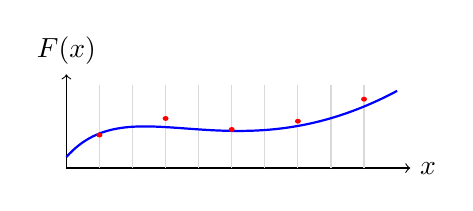
\begin{tikzpicture}[x=0.42cm,y=0.35cm]
 \draw[->] (0,0)--(10.4,0) node[right] {$x$};
 \draw[->] (0,0)--(0,3.4) node[above] {$F(x)$};
 \foreach \x in {1,...,9} {\draw[gray!30] (\x,0)--(\x,3);}
 \draw[blue,thick] (0,0.4) .. controls (2,3.1) and (5,-0.4) .. (10,2.8);
 \foreach \x/\y in {1/1.2,3/1.8,5/1.4,7/1.7,9/2.5}
   \fill[red] (\x,\y) circle (0.09);
\end{tikzpicture}
\end{center}
The next comparison uses Theorem~\ref{thm:2} and Equation~\ref{eq:3}. The construction uses a finite family of examples with different paragraph lengths. Some sentences are short. Others follow the dependence of an estimate on its parameters, introduce a counterexample, and explain why a nearby bound must be reconsidered after an insertion.

\lipsum[18]

\section{A changing estimate: case 005}\label{unit:4}
A local change should remain attached to its source even when surrounding material moves. We compare the displayed argument with the current source version, rather than treating the last compiled page number as a permanent identity.

\lipsum[13-14]
\begin{align}\label{eq:4}
 F_k(x+h)&=F_k(x)+hF_k'(x)+\frac{h^2}{2}F_k''(x)+O(h^3),\\
 \int_0^1 t^k(1-t)\,dt&=\frac{1}{(k+1)(k+2)}.
\end{align}
\begin{theorem}\label{thm:4}
For the finite family in case 5, the normalized error is bounded by $C_k h^2$ whenever $0<h<1$. The constant may depend on $k$ but is independent of the location of the edited paragraph.
\end{theorem}
\begin{proof}
Expand the two terms, collect their first-order contributions, and apply the
triangle inequality. The remaining integral is bounded on the compact interval,
so the asserted estimate follows. This argument also applies after a line break
moves the statement to the next page.
\end{proof}
The next comparison uses Theorem~\ref{thm:3} and Equation~\ref{eq:4}. An observer can return to an earlier part of the document while compilation continues. The relevant statement, equation and hyperlink must still belong to the page actually displayed, including when line wrapping pushes a later theorem across a page boundary.

\lipsum[23]

\section{A changing estimate: case 006}\label{unit:5}
The construction uses a finite family of examples with different paragraph lengths. Some sentences are short. Others follow the dependence of an estimate on its parameters, introduce a counterexample, and explain why a nearby bound must be reconsidered after an insertion.

\lipsum[16-17]
\begin{align}\label{eq:5}
 F_k(x+h)&=F_k(x)+hF_k'(x)+\frac{h^2}{2}F_k''(x)+O(h^3),\\
 \int_0^1 t^k(1-t)\,dt&=\frac{1}{(k+1)(k+2)}.
\end{align}
\begin{theorem}\label{thm:5}
For the finite family in case 6, the normalized error is bounded by $C_k h^2$ whenever $0<h<1$. The constant may depend on $k$ but is independent of the location of the edited paragraph.
\end{theorem}
\begin{proof}
Expand the two terms, collect their first-order contributions, and apply the
triangle inequality. The remaining integral is bounded on the compact interval,
so the asserted estimate follows. This argument also applies after a line break
moves the statement to the next page.
\end{proof}
The next comparison uses Theorem~\ref{thm:4} and Equation~\ref{eq:5}. The proof separates the algebraic estimate from the geometric example. This makes the document useful for edits to prose, formulas, headings and diagrams, while retaining enough ordinary text to exercise paragraph breaking and natural pagination.

\lipsum[3]

\section{A changing estimate: case 007}\label{unit:6}
An observer can return to an earlier part of the document while compilation continues. The relevant statement, equation and hyperlink must still belong to the page actually displayed, including when line wrapping pushes a later theorem across a page boundary.

\lipsum[19-20]
\begin{align}\label{eq:6}
 F_k(x+h)&=F_k(x)+hF_k'(x)+\frac{h^2}{2}F_k''(x)+O(h^3),\\
 \int_0^1 t^k(1-t)\,dt&=\frac{1}{(k+1)(k+2)}.
\end{align}
\begin{lemma}\label{thm:6}
For the finite family in case 7, the normalized error is bounded by $C_k h^2$ whenever $0<h<1$. The constant may depend on $k$ but is independent of the location of the edited paragraph.
\end{lemma}
\begin{proof}
Expand the two terms, collect their first-order contributions, and apply the
triangle inequality. The remaining integral is bounded on the compact interval,
so the asserted estimate follows. This argument also applies after a line break
moves the statement to the next page.
\end{proof}
The next comparison uses Theorem~\ref{thm:5} and Equation~\ref{eq:6}. A local change should remain attached to its source even when surrounding material moves. We compare the displayed argument with the current source version, rather than treating the last compiled page number as a permanent identity.

\lipsum[8]

\section{A changing estimate: case 008}\label{unit:7}
The proof separates the algebraic estimate from the geometric example. This makes the document useful for edits to prose, formulas, headings and diagrams, while retaining enough ordinary text to exercise paragraph breaking and natural pagination.

\lipsum[22-23]
\begin{align}\label{eq:7}
 F_k(x+h)&=F_k(x)+hF_k'(x)+\frac{h^2}{2}F_k''(x)+O(h^3),\\
 \int_0^1 t^k(1-t)\,dt&=\frac{1}{(k+1)(k+2)}.
\end{align}
\begin{theorem}\label{thm:7}
For the finite family in case 8, the normalized error is bounded by $C_k h^2$ whenever $0<h<1$. The constant may depend on $k$ but is independent of the location of the edited paragraph.
\end{theorem}
\begin{proof}
Expand the two terms, collect their first-order contributions, and apply the
triangle inequality. The remaining integral is bounded on the compact interval,
so the asserted estimate follows. This argument also applies after a line break
moves the statement to the next page.
\end{proof}
The next comparison uses Theorem~\ref{thm:6} and Equation~\ref{eq:7}. The construction uses a finite family of examples with different paragraph lengths. Some sentences are short. Others follow the dependence of an estimate on its parameters, introduce a counterexample, and explain why a nearby bound must be reconsidered after an insertion.

\lipsum[13]

\section{A changing estimate: case 009}\label{unit:8}
A local change should remain attached to its source even when surrounding material moves. We compare the displayed argument with the current source version, rather than treating the last compiled page number as a permanent identity.

\lipsum[25-26]
\begin{align}\label{eq:8}
 F_k(x+h)&=F_k(x)+hF_k'(x)+\frac{h^2}{2}F_k''(x)+O(h^3),\\
 \int_0^1 t^k(1-t)\,dt&=\frac{1}{(k+1)(k+2)}.
\end{align}
\begin{theorem}\label{thm:8}
For the finite family in case 9, the normalized error is bounded by $C_k h^2$ whenever $0<h<1$. The constant may depend on $k$ but is independent of the location of the edited paragraph.
\end{theorem}
\begin{proof}
Expand the two terms, collect their first-order contributions, and apply the
triangle inequality. The remaining integral is bounded on the compact interval,
so the asserted estimate follows. This argument also applies after a line break
moves the statement to the next page.
\end{proof}
The next comparison uses Theorem~\ref{thm:7} and Equation~\ref{eq:8}. An observer can return to an earlier part of the document while compilation continues. The relevant statement, equation and hyperlink must still belong to the page actually displayed, including when line wrapping pushes a later theorem across a page boundary.

\lipsum[18]

\section{A changing estimate: case 010}\label{unit:9}
The construction uses a finite family of examples with different paragraph lengths. Some sentences are short. Others follow the dependence of an estimate on its parameters, introduce a counterexample, and explain why a nearby bound must be reconsidered after an insertion.

\lipsum[28-29]
\begin{align}\label{eq:9}
 F_k(x+h)&=F_k(x)+hF_k'(x)+\frac{h^2}{2}F_k''(x)+O(h^3),\\
 \int_0^1 t^k(1-t)\,dt&=\frac{1}{(k+1)(k+2)}.
\end{align}
\begin{lemma}\label{thm:9}
For the finite family in case 10, the normalized error is bounded by $C_k h^2$ whenever $0<h<1$. The constant may depend on $k$ but is independent of the location of the edited paragraph.
\end{lemma}
\begin{proof}
Expand the two terms, collect their first-order contributions, and apply the
triangle inequality. The remaining integral is bounded on the compact interval,
so the asserted estimate follows. This argument also applies after a line break
moves the statement to the next page.
\end{proof}
\begin{center}
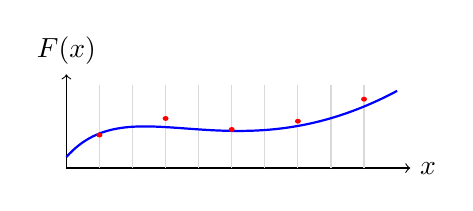
\begin{tikzpicture}[x=0.42cm,y=0.35cm]
 \draw[->] (0,0)--(10.4,0) node[right] {$x$};
 \draw[->] (0,0)--(0,3.4) node[above] {$F(x)$};
 \foreach \x in {1,...,9} {\draw[gray!30] (\x,0)--(\x,3);}
 \draw[blue,thick] (0,0.4) .. controls (2,3.1) and (5,-0.4) .. (10,2.8);
 \foreach \x/\y in {1/1.2,3/1.8,5/1.4,7/1.7,9/2.5}
   \fill[red] (\x,\y) circle (0.09);
\end{tikzpicture}
\end{center}
The next comparison uses Theorem~\ref{thm:8} and Equation~\ref{eq:9}. The proof separates the algebraic estimate from the geometric example. This makes the document useful for edits to prose, formulas, headings and diagrams, while retaining enough ordinary text to exercise paragraph breaking and natural pagination.

\lipsum[23]

\section{A changing estimate: case 011}\label{unit:10}
An observer can return to an earlier part of the document while compilation continues. The relevant statement, equation and hyperlink must still belong to the page actually displayed, including when line wrapping pushes a later theorem across a page boundary.

\lipsum[1-2]
\begin{align}\label{eq:10}
 F_k(x+h)&=F_k(x)+hF_k'(x)+\frac{h^2}{2}F_k''(x)+O(h^3),\\
 \int_0^1 t^k(1-t)\,dt&=\frac{1}{(k+1)(k+2)}.
\end{align}
\begin{theorem}\label{thm:10}
For the finite family in case 11, the normalized error is bounded by $C_k h^2$ whenever $0<h<1$. The constant may depend on $k$ but is independent of the location of the edited paragraph.
\end{theorem}
\begin{proof}
Expand the two terms, collect their first-order contributions, and apply the
triangle inequality. The remaining integral is bounded on the compact interval,
so the asserted estimate follows. This argument also applies after a line break
moves the statement to the next page.
\end{proof}
The next comparison uses Theorem~\ref{thm:9} and Equation~\ref{eq:10}. A local change should remain attached to its source even when surrounding material moves. We compare the displayed argument with the current source version, rather than treating the last compiled page number as a permanent identity.

\lipsum[3]

\section{A changing estimate: case 012}\label{unit:11}
The proof separates the algebraic estimate from the geometric example. This makes the document useful for edits to prose, formulas, headings and diagrams, while retaining enough ordinary text to exercise paragraph breaking and natural pagination.

\lipsum[4-5]
\begin{align}\label{eq:11}
 F_k(x+h)&=F_k(x)+hF_k'(x)+\frac{h^2}{2}F_k''(x)+O(h^3),\\
 \int_0^1 t^k(1-t)\,dt&=\frac{1}{(k+1)(k+2)}.
\end{align}
\begin{theorem}\label{thm:11}
For the finite family in case 12, the normalized error is bounded by $C_k h^2$ whenever $0<h<1$. The constant may depend on $k$ but is independent of the location of the edited paragraph.
\end{theorem}
\begin{proof}
Expand the two terms, collect their first-order contributions, and apply the
triangle inequality. The remaining integral is bounded on the compact interval,
so the asserted estimate follows. This argument also applies after a line break
moves the statement to the next page.
\end{proof}
The next comparison uses Theorem~\ref{thm:10} and Equation~\ref{eq:11}. The construction uses a finite family of examples with different paragraph lengths. Some sentences are short. Others follow the dependence of an estimate on its parameters, introduce a counterexample, and explain why a nearby bound must be reconsidered after an insertion.

\lipsum[8]

\section{A changing estimate: case 013}\label{unit:12}
A local change should remain attached to its source even when surrounding material moves. We compare the displayed argument with the current source version, rather than treating the last compiled page number as a permanent identity.

\lipsum[7-8]
\begin{align}\label{eq:12}
 F_k(x+h)&=F_k(x)+hF_k'(x)+\frac{h^2}{2}F_k''(x)+O(h^3),\\
 \int_0^1 t^k(1-t)\,dt&=\frac{1}{(k+1)(k+2)}.
\end{align}
\begin{lemma}\label{thm:12}
For the finite family in case 13, the normalized error is bounded by $C_k h^2$ whenever $0<h<1$. The constant may depend on $k$ but is independent of the location of the edited paragraph.
\end{lemma}
\begin{proof}
Expand the two terms, collect their first-order contributions, and apply the
triangle inequality. The remaining integral is bounded on the compact interval,
so the asserted estimate follows. This argument also applies after a line break
moves the statement to the next page.
\end{proof}
The next comparison uses Theorem~\ref{thm:11} and Equation~\ref{eq:12}. An observer can return to an earlier part of the document while compilation continues. The relevant statement, equation and hyperlink must still belong to the page actually displayed, including when line wrapping pushes a later theorem across a page boundary.

\lipsum[13]

\section{A changing estimate: case 014}\label{unit:13}
The construction uses a finite family of examples with different paragraph lengths. Some sentences are short. Others follow the dependence of an estimate on its parameters, introduce a counterexample, and explain why a nearby bound must be reconsidered after an insertion.

\lipsum[10-11]
\begin{align}\label{eq:13}
 F_k(x+h)&=F_k(x)+hF_k'(x)+\frac{h^2}{2}F_k''(x)+O(h^3),\\
 \int_0^1 t^k(1-t)\,dt&=\frac{1}{(k+1)(k+2)}.
\end{align}
\begin{theorem}\label{thm:13}
For the finite family in case 14, the normalized error is bounded by $C_k h^2$ whenever $0<h<1$. The constant may depend on $k$ but is independent of the location of the edited paragraph.
\end{theorem}
\begin{proof}
Expand the two terms, collect their first-order contributions, and apply the
triangle inequality. The remaining integral is bounded on the compact interval,
so the asserted estimate follows. This argument also applies after a line break
moves the statement to the next page.
\end{proof}
The next comparison uses Theorem~\ref{thm:12} and Equation~\ref{eq:13}. The proof separates the algebraic estimate from the geometric example. This makes the document useful for edits to prose, formulas, headings and diagrams, while retaining enough ordinary text to exercise paragraph breaking and natural pagination.

\lipsum[18]

\section{A changing estimate: case 015}\label{unit:14}
An observer can return to an earlier part of the document while compilation continues. The relevant statement, equation and hyperlink must still belong to the page actually displayed, including when line wrapping pushes a later theorem across a page boundary.

\lipsum[13-14]
\begin{align}\label{eq:14}
 F_k(x+h)&=F_k(x)+hF_k'(x)+\frac{h^2}{2}F_k''(x)+O(h^3),\\
 \int_0^1 t^k(1-t)\,dt&=\frac{1}{(k+1)(k+2)}.
\end{align}
\begin{theorem}\label{thm:14}
For the finite family in case 15, the normalized error is bounded by $C_k h^2$ whenever $0<h<1$. The constant may depend on $k$ but is independent of the location of the edited paragraph.
\end{theorem}
\begin{proof}
Expand the two terms, collect their first-order contributions, and apply the
triangle inequality. The remaining integral is bounded on the compact interval,
so the asserted estimate follows. This argument also applies after a line break
moves the statement to the next page.
\end{proof}
The next comparison uses Theorem~\ref{thm:13} and Equation~\ref{eq:14}. A local change should remain attached to its source even when surrounding material moves. We compare the displayed argument with the current source version, rather than treating the last compiled page number as a permanent identity.

\lipsum[23]

\section{A changing estimate: case 016}\label{unit:15}
The proof separates the algebraic estimate from the geometric example. This makes the document useful for edits to prose, formulas, headings and diagrams, while retaining enough ordinary text to exercise paragraph breaking and natural pagination.

\lipsum[16-17]
\begin{align}\label{eq:15}
 F_k(x+h)&=F_k(x)+hF_k'(x)+\frac{h^2}{2}F_k''(x)+O(h^3),\\
 \int_0^1 t^k(1-t)\,dt&=\frac{1}{(k+1)(k+2)}.
\end{align}
\begin{lemma}\label{thm:15}
For the finite family in case 16, the normalized error is bounded by $C_k h^2$ whenever $0<h<1$. The constant may depend on $k$ but is independent of the location of the edited paragraph.
\end{lemma}
\begin{proof}
Expand the two terms, collect their first-order contributions, and apply the
triangle inequality. The remaining integral is bounded on the compact interval,
so the asserted estimate follows. This argument also applies after a line break
moves the statement to the next page.
\end{proof}
\begin{center}
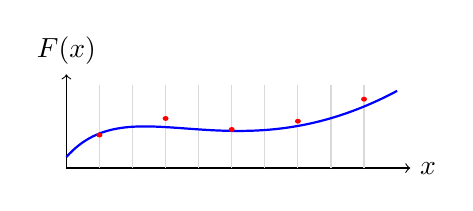
\begin{tikzpicture}[x=0.42cm,y=0.35cm]
 \draw[->] (0,0)--(10.4,0) node[right] {$x$};
 \draw[->] (0,0)--(0,3.4) node[above] {$F(x)$};
 \foreach \x in {1,...,9} {\draw[gray!30] (\x,0)--(\x,3);}
 \draw[blue,thick] (0,0.4) .. controls (2,3.1) and (5,-0.4) .. (10,2.8);
 \foreach \x/\y in {1/1.2,3/1.8,5/1.4,7/1.7,9/2.5}
   \fill[red] (\x,\y) circle (0.09);
\end{tikzpicture}
\end{center}
The next comparison uses Theorem~\ref{thm:14} and Equation~\ref{eq:15}. The construction uses a finite family of examples with different paragraph lengths. Some sentences are short. Others follow the dependence of an estimate on its parameters, introduce a counterexample, and explain why a nearby bound must be reconsidered after an insertion.

\lipsum[3]

\section{A changing estimate: case 017}\label{unit:16}
A local change should remain attached to its source even when surrounding material moves. We compare the displayed argument with the current source version, rather than treating the last compiled page number as a permanent identity.

\lipsum[19-20]
\begin{align}\label{eq:16}
 F_k(x+h)&=F_k(x)+hF_k'(x)+\frac{h^2}{2}F_k''(x)+O(h^3),\\
 \int_0^1 t^k(1-t)\,dt&=\frac{1}{(k+1)(k+2)}.
\end{align}
\begin{theorem}\label{thm:16}
For the finite family in case 17, the normalized error is bounded by $C_k h^2$ whenever $0<h<1$. The constant may depend on $k$ but is independent of the location of the edited paragraph.
\end{theorem}
\begin{proof}
Expand the two terms, collect their first-order contributions, and apply the
triangle inequality. The remaining integral is bounded on the compact interval,
so the asserted estimate follows. This argument also applies after a line break
moves the statement to the next page.
\end{proof}
The next comparison uses Theorem~\ref{thm:15} and Equation~\ref{eq:16}. An observer can return to an earlier part of the document while compilation continues. The relevant statement, equation and hyperlink must still belong to the page actually displayed, including when line wrapping pushes a later theorem across a page boundary.

\lipsum[8]

\section{A changing estimate: case 018}\label{unit:17}
The construction uses a finite family of examples with different paragraph lengths. Some sentences are short. Others follow the dependence of an estimate on its parameters, introduce a counterexample, and explain why a nearby bound must be reconsidered after an insertion.

\lipsum[22-23]
\begin{align}\label{eq:17}
 F_k(x+h)&=F_k(x)+hF_k'(x)+\frac{h^2}{2}F_k''(x)+O(h^3),\\
 \int_0^1 t^k(1-t)\,dt&=\frac{1}{(k+1)(k+2)}.
\end{align}
\begin{theorem}\label{thm:17}
For the finite family in case 18, the normalized error is bounded by $C_k h^2$ whenever $0<h<1$. The constant may depend on $k$ but is independent of the location of the edited paragraph.
\end{theorem}
\begin{proof}
Expand the two terms, collect their first-order contributions, and apply the
triangle inequality. The remaining integral is bounded on the compact interval,
so the asserted estimate follows. This argument also applies after a line break
moves the statement to the next page.
\end{proof}
The next comparison uses Theorem~\ref{thm:16} and Equation~\ref{eq:17}. The proof separates the algebraic estimate from the geometric example. This makes the document useful for edits to prose, formulas, headings and diagrams, while retaining enough ordinary text to exercise paragraph breaking and natural pagination.

\lipsum[13]

\section{A changing estimate: case 019}\label{unit:18}
An observer can return to an earlier part of the document while compilation continues. The relevant statement, equation and hyperlink must still belong to the page actually displayed, including when line wrapping pushes a later theorem across a page boundary.

\lipsum[25-26]
\begin{align}\label{eq:18}
 F_k(x+h)&=F_k(x)+hF_k'(x)+\frac{h^2}{2}F_k''(x)+O(h^3),\\
 \int_0^1 t^k(1-t)\,dt&=\frac{1}{(k+1)(k+2)}.
\end{align}
\begin{lemma}\label{thm:18}
For the finite family in case 19, the normalized error is bounded by $C_k h^2$ whenever $0<h<1$. The constant may depend on $k$ but is independent of the location of the edited paragraph.
\end{lemma}
\begin{proof}
Expand the two terms, collect their first-order contributions, and apply the
triangle inequality. The remaining integral is bounded on the compact interval,
so the asserted estimate follows. This argument also applies after a line break
moves the statement to the next page.
\end{proof}
The next comparison uses Theorem~\ref{thm:17} and Equation~\ref{eq:18}. A local change should remain attached to its source even when surrounding material moves. We compare the displayed argument with the current source version, rather than treating the last compiled page number as a permanent identity.

\lipsum[18]

\section{A changing estimate: case 020}\label{unit:19}
The proof separates the algebraic estimate from the geometric example. This makes the document useful for edits to prose, formulas, headings and diagrams, while retaining enough ordinary text to exercise paragraph breaking and natural pagination.

\lipsum[28-29]
\begin{align}\label{eq:19}
 F_k(x+h)&=F_k(x)+hF_k'(x)+\frac{h^2}{2}F_k''(x)+O(h^3),\\
 \int_0^1 t^k(1-t)\,dt&=\frac{1}{(k+1)(k+2)}.
\end{align}
\begin{theorem}\label{thm:19}
For the finite family in case 20, the normalized error is bounded by $C_k h^2$ whenever $0<h<1$. The constant may depend on $k$ but is independent of the location of the edited paragraph.
\end{theorem}
\begin{proof}
Expand the two terms, collect their first-order contributions, and apply the
triangle inequality. The remaining integral is bounded on the compact interval,
so the asserted estimate follows. This argument also applies after a line break
moves the statement to the next page.
\end{proof}
The next comparison uses Theorem~\ref{thm:18} and Equation~\ref{eq:19}. The construction uses a finite family of examples with different paragraph lengths. Some sentences are short. Others follow the dependence of an estimate on its parameters, introduce a counterexample, and explain why a nearby bound must be reconsidered after an insertion.

\lipsum[23]

\section{A changing estimate: case 021}\label{unit:20}
A local change should remain attached to its source even when surrounding material moves. We compare the displayed argument with the current source version, rather than treating the last compiled page number as a permanent identity.

\lipsum[1-2]
\begin{align}\label{eq:20}
 F_k(x+h)&=F_k(x)+hF_k'(x)+\frac{h^2}{2}F_k''(x)+O(h^3),\\
 \int_0^1 t^k(1-t)\,dt&=\frac{1}{(k+1)(k+2)}.
\end{align}
\begin{theorem}\label{thm:20}
For the finite family in case 21, the normalized error is bounded by $C_k h^2$ whenever $0<h<1$. The constant may depend on $k$ but is independent of the location of the edited paragraph.
\end{theorem}
\begin{proof}
Expand the two terms, collect their first-order contributions, and apply the
triangle inequality. The remaining integral is bounded on the compact interval,
so the asserted estimate follows. This argument also applies after a line break
moves the statement to the next page.
\end{proof}
The next comparison uses Theorem~\ref{thm:19} and Equation~\ref{eq:20}. An observer can return to an earlier part of the document while compilation continues. The relevant statement, equation and hyperlink must still belong to the page actually displayed, including when line wrapping pushes a later theorem across a page boundary.

\lipsum[3]

\section{A changing estimate: case 022}\label{unit:21}
The construction uses a finite family of examples with different paragraph lengths. Some sentences are short. Others follow the dependence of an estimate on its parameters, introduce a counterexample, and explain why a nearby bound must be reconsidered after an insertion.

\lipsum[4-5]
\begin{align}\label{eq:21}
 F_k(x+h)&=F_k(x)+hF_k'(x)+\frac{h^2}{2}F_k''(x)+O(h^3),\\
 \int_0^1 t^k(1-t)\,dt&=\frac{1}{(k+1)(k+2)}.
\end{align}
\begin{lemma}\label{thm:21}
For the finite family in case 22, the normalized error is bounded by $C_k h^2$ whenever $0<h<1$. The constant may depend on $k$ but is independent of the location of the edited paragraph.
\end{lemma}
\begin{proof}
Expand the two terms, collect their first-order contributions, and apply the
triangle inequality. The remaining integral is bounded on the compact interval,
so the asserted estimate follows. This argument also applies after a line break
moves the statement to the next page.
\end{proof}
\begin{center}
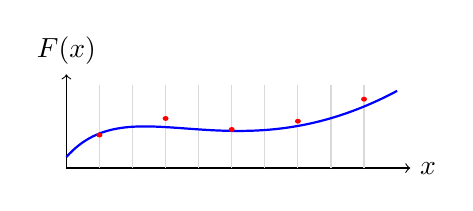
\begin{tikzpicture}[x=0.42cm,y=0.35cm]
 \draw[->] (0,0)--(10.4,0) node[right] {$x$};
 \draw[->] (0,0)--(0,3.4) node[above] {$F(x)$};
 \foreach \x in {1,...,9} {\draw[gray!30] (\x,0)--(\x,3);}
 \draw[blue,thick] (0,0.4) .. controls (2,3.1) and (5,-0.4) .. (10,2.8);
 \foreach \x/\y in {1/1.2,3/1.8,5/1.4,7/1.7,9/2.5}
   \fill[red] (\x,\y) circle (0.09);
\end{tikzpicture}
\end{center}
The next comparison uses Theorem~\ref{thm:20} and Equation~\ref{eq:21}. The proof separates the algebraic estimate from the geometric example. This makes the document useful for edits to prose, formulas, headings and diagrams, while retaining enough ordinary text to exercise paragraph breaking and natural pagination.

\lipsum[8]

\section{A changing estimate: case 023}\label{unit:22}
An observer can return to an earlier part of the document while compilation continues. The relevant statement, equation and hyperlink must still belong to the page actually displayed, including when line wrapping pushes a later theorem across a page boundary.

\lipsum[7-8]
\begin{align}\label{eq:22}
 F_k(x+h)&=F_k(x)+hF_k'(x)+\frac{h^2}{2}F_k''(x)+O(h^3),\\
 \int_0^1 t^k(1-t)\,dt&=\frac{1}{(k+1)(k+2)}.
\end{align}
\begin{theorem}\label{thm:22}
For the finite family in case 23, the normalized error is bounded by $C_k h^2$ whenever $0<h<1$. The constant may depend on $k$ but is independent of the location of the edited paragraph.
\end{theorem}
\begin{proof}
Expand the two terms, collect their first-order contributions, and apply the
triangle inequality. The remaining integral is bounded on the compact interval,
so the asserted estimate follows. This argument also applies after a line break
moves the statement to the next page.
\end{proof}
The next comparison uses Theorem~\ref{thm:21} and Equation~\ref{eq:22}. A local change should remain attached to its source even when surrounding material moves. We compare the displayed argument with the current source version, rather than treating the last compiled page number as a permanent identity.

\lipsum[13]

\section{A changing estimate: case 024}\label{unit:23}
The proof separates the algebraic estimate from the geometric example. This makes the document useful for edits to prose, formulas, headings and diagrams, while retaining enough ordinary text to exercise paragraph breaking and natural pagination.

\lipsum[10-11]
\begin{align}\label{eq:23}
 F_k(x+h)&=F_k(x)+hF_k'(x)+\frac{h^2}{2}F_k''(x)+O(h^3),\\
 \int_0^1 t^k(1-t)\,dt&=\frac{1}{(k+1)(k+2)}.
\end{align}
\begin{theorem}\label{thm:23}
For the finite family in case 24, the normalized error is bounded by $C_k h^2$ whenever $0<h<1$. The constant may depend on $k$ but is independent of the location of the edited paragraph.
\end{theorem}
\begin{proof}
Expand the two terms, collect their first-order contributions, and apply the
triangle inequality. The remaining integral is bounded on the compact interval,
so the asserted estimate follows. This argument also applies after a line break
moves the statement to the next page.
\end{proof}
The next comparison uses Theorem~\ref{thm:22} and Equation~\ref{eq:23}. The construction uses a finite family of examples with different paragraph lengths. Some sentences are short. Others follow the dependence of an estimate on its parameters, introduce a counterexample, and explain why a nearby bound must be reconsidered after an insertion.

\lipsum[18]

\section{A changing estimate: case 025}\label{unit:24}
A local change should remain attached to its source even when surrounding material moves. We compare the displayed argument with the current source version, rather than treating the last compiled page number as a permanent identity.

\lipsum[13-14]
\begin{align}\label{eq:24}
 F_k(x+h)&=F_k(x)+hF_k'(x)+\frac{h^2}{2}F_k''(x)+O(h^3),\\
 \int_0^1 t^k(1-t)\,dt&=\frac{1}{(k+1)(k+2)}.
\end{align}
\begin{lemma}\label{thm:24}
For the finite family in case 25, the normalized error is bounded by $C_k h^2$ whenever $0<h<1$. The constant may depend on $k$ but is independent of the location of the edited paragraph.
\end{lemma}
\begin{proof}
Expand the two terms, collect their first-order contributions, and apply the
triangle inequality. The remaining integral is bounded on the compact interval,
so the asserted estimate follows. This argument also applies after a line break
moves the statement to the next page.
\end{proof}
The next comparison uses Theorem~\ref{thm:23} and Equation~\ref{eq:24}. An observer can return to an earlier part of the document while compilation continues. The relevant statement, equation and hyperlink must still belong to the page actually displayed, including when line wrapping pushes a later theorem across a page boundary.

\lipsum[23]

\section{A changing estimate: case 026}\label{unit:25}
The construction uses a finite family of examples with different paragraph lengths. Some sentences are short. Others follow the dependence of an estimate on its parameters, introduce a counterexample, and explain why a nearby bound must be reconsidered after an insertion.

\lipsum[16-17]
\begin{align}\label{eq:25}
 F_k(x+h)&=F_k(x)+hF_k'(x)+\frac{h^2}{2}F_k''(x)+O(h^3),\\
 \int_0^1 t^k(1-t)\,dt&=\frac{1}{(k+1)(k+2)}.
\end{align}
\begin{theorem}\label{thm:25}
For the finite family in case 26, the normalized error is bounded by $C_k h^2$ whenever $0<h<1$. The constant may depend on $k$ but is independent of the location of the edited paragraph.
\end{theorem}
\begin{proof}
Expand the two terms, collect their first-order contributions, and apply the
triangle inequality. The remaining integral is bounded on the compact interval,
so the asserted estimate follows. This argument also applies after a line break
moves the statement to the next page.
\end{proof}
The next comparison uses Theorem~\ref{thm:24} and Equation~\ref{eq:25}. The proof separates the algebraic estimate from the geometric example. This makes the document useful for edits to prose, formulas, headings and diagrams, while retaining enough ordinary text to exercise paragraph breaking and natural pagination.

\lipsum[3]

\section{A changing estimate: case 027}\label{unit:26}
An observer can return to an earlier part of the document while compilation continues. The relevant statement, equation and hyperlink must still belong to the page actually displayed, including when line wrapping pushes a later theorem across a page boundary.

\lipsum[19-20]
\begin{align}\label{eq:26}
 F_k(x+h)&=F_k(x)+hF_k'(x)+\frac{h^2}{2}F_k''(x)+O(h^3),\\
 \int_0^1 t^k(1-t)\,dt&=\frac{1}{(k+1)(k+2)}.
\end{align}
\begin{theorem}\label{thm:26}
For the finite family in case 27, the normalized error is bounded by $C_k h^2$ whenever $0<h<1$. The constant may depend on $k$ but is independent of the location of the edited paragraph.
\end{theorem}
\begin{proof}
Expand the two terms, collect their first-order contributions, and apply the
triangle inequality. The remaining integral is bounded on the compact interval,
so the asserted estimate follows. This argument also applies after a line break
moves the statement to the next page.
\end{proof}
The next comparison uses Theorem~\ref{thm:25} and Equation~\ref{eq:26}. A local change should remain attached to its source even when surrounding material moves. We compare the displayed argument with the current source version, rather than treating the last compiled page number as a permanent identity.

\lipsum[8]

\section{A changing estimate: case 028}\label{unit:27}
The proof separates the algebraic estimate from the geometric example. This makes the document useful for edits to prose, formulas, headings and diagrams, while retaining enough ordinary text to exercise paragraph breaking and natural pagination.

\lipsum[22-23]
\begin{align}\label{eq:27}
 F_k(x+h)&=F_k(x)+hF_k'(x)+\frac{h^2}{2}F_k''(x)+O(h^3),\\
 \int_0^1 t^k(1-t)\,dt&=\frac{1}{(k+1)(k+2)}.
\end{align}
\begin{lemma}\label{thm:27}
For the finite family in case 28, the normalized error is bounded by $C_k h^2$ whenever $0<h<1$. The constant may depend on $k$ but is independent of the location of the edited paragraph.
\end{lemma}
\begin{proof}
Expand the two terms, collect their first-order contributions, and apply the
triangle inequality. The remaining integral is bounded on the compact interval,
so the asserted estimate follows. This argument also applies after a line break
moves the statement to the next page.
\end{proof}
\begin{center}
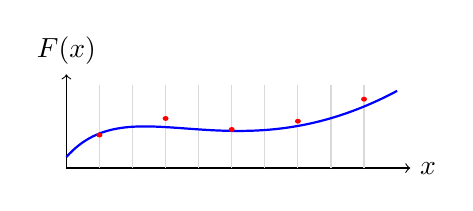
\begin{tikzpicture}[x=0.42cm,y=0.35cm]
 \draw[->] (0,0)--(10.4,0) node[right] {$x$};
 \draw[->] (0,0)--(0,3.4) node[above] {$F(x)$};
 \foreach \x in {1,...,9} {\draw[gray!30] (\x,0)--(\x,3);}
 \draw[blue,thick] (0,0.4) .. controls (2,3.1) and (5,-0.4) .. (10,2.8);
 \foreach \x/\y in {1/1.2,3/1.8,5/1.4,7/1.7,9/2.5}
   \fill[red] (\x,\y) circle (0.09);
\end{tikzpicture}
\end{center}
The next comparison uses Theorem~\ref{thm:26} and Equation~\ref{eq:27}. The construction uses a finite family of examples with different paragraph lengths. Some sentences are short. Others follow the dependence of an estimate on its parameters, introduce a counterexample, and explain why a nearby bound must be reconsidered after an insertion.

\lipsum[13]

\section{A changing estimate: case 029}\label{unit:28}
A local change should remain attached to its source even when surrounding material moves. We compare the displayed argument with the current source version, rather than treating the last compiled page number as a permanent identity.

\lipsum[25-26]
\begin{align}\label{eq:28}
 F_k(x+h)&=F_k(x)+hF_k'(x)+\frac{h^2}{2}F_k''(x)+O(h^3),\\
 \int_0^1 t^k(1-t)\,dt&=\frac{1}{(k+1)(k+2)}.
\end{align}
\begin{theorem}\label{thm:28}
For the finite family in case 29, the normalized error is bounded by $C_k h^2$ whenever $0<h<1$. The constant may depend on $k$ but is independent of the location of the edited paragraph.
\end{theorem}
\begin{proof}
Expand the two terms, collect their first-order contributions, and apply the
triangle inequality. The remaining integral is bounded on the compact interval,
so the asserted estimate follows. This argument also applies after a line break
moves the statement to the next page.
\end{proof}
The next comparison uses Theorem~\ref{thm:27} and Equation~\ref{eq:28}. An observer can return to an earlier part of the document while compilation continues. The relevant statement, equation and hyperlink must still belong to the page actually displayed, including when line wrapping pushes a later theorem across a page boundary.

\lipsum[18]

\section{A changing estimate: case 030}\label{unit:29}
The construction uses a finite family of examples with different paragraph lengths. Some sentences are short. Others follow the dependence of an estimate on its parameters, introduce a counterexample, and explain why a nearby bound must be reconsidered after an insertion.

\lipsum[28-29]
\begin{align}\label{eq:29}
 F_k(x+h)&=F_k(x)+hF_k'(x)+\frac{h^2}{2}F_k''(x)+O(h^3),\\
 \int_0^1 t^k(1-t)\,dt&=\frac{1}{(k+1)(k+2)}.
\end{align}
\begin{theorem}\label{thm:29}
For the finite family in case 30, the normalized error is bounded by $C_k h^2$ whenever $0<h<1$. The constant may depend on $k$ but is independent of the location of the edited paragraph.
\end{theorem}
\begin{proof}
Expand the two terms, collect their first-order contributions, and apply the
triangle inequality. The remaining integral is bounded on the compact interval,
so the asserted estimate follows. This argument also applies after a line break
moves the statement to the next page.
\end{proof}
The next comparison uses Theorem~\ref{thm:28} and Equation~\ref{eq:29}. The proof separates the algebraic estimate from the geometric example. This makes the document useful for edits to prose, formulas, headings and diagrams, while retaining enough ordinary text to exercise paragraph breaking and natural pagination.

\lipsum[23]

\section{A changing estimate: case 031}\label{unit:30}
An observer can return to an earlier part of the document while compilation continues. The relevant statement, equation and hyperlink must still belong to the page actually displayed, including when line wrapping pushes a later theorem across a page boundary.

\lipsum[1-2]
\begin{align}\label{eq:30}
 F_k(x+h)&=F_k(x)+hF_k'(x)+\frac{h^2}{2}F_k''(x)+O(h^3),\\
 \int_0^1 t^k(1-t)\,dt&=\frac{1}{(k+1)(k+2)}.
\end{align}
\begin{lemma}\label{thm:30}
For the finite family in case 31, the normalized error is bounded by $C_k h^2$ whenever $0<h<1$. The constant may depend on $k$ but is independent of the location of the edited paragraph.
\end{lemma}
\begin{proof}
Expand the two terms, collect their first-order contributions, and apply the
triangle inequality. The remaining integral is bounded on the compact interval,
so the asserted estimate follows. This argument also applies after a line break
moves the statement to the next page.
\end{proof}
The next comparison uses Theorem~\ref{thm:29} and Equation~\ref{eq:30}. A local change should remain attached to its source even when surrounding material moves. We compare the displayed argument with the current source version, rather than treating the last compiled page number as a permanent identity.

\lipsum[3]

\section{A changing estimate: case 032}\label{unit:31}
The proof separates the algebraic estimate from the geometric example. This makes the document useful for edits to prose, formulas, headings and diagrams, while retaining enough ordinary text to exercise paragraph breaking and natural pagination.

\lipsum[4-5]
\begin{align}\label{eq:31}
 F_k(x+h)&=F_k(x)+hF_k'(x)+\frac{h^2}{2}F_k''(x)+O(h^3),\\
 \int_0^1 t^k(1-t)\,dt&=\frac{1}{(k+1)(k+2)}.
\end{align}
\begin{theorem}\label{thm:31}
For the finite family in case 32, the normalized error is bounded by $C_k h^2$ whenever $0<h<1$. The constant may depend on $k$ but is independent of the location of the edited paragraph.
\end{theorem}
\begin{proof}
Expand the two terms, collect their first-order contributions, and apply the
triangle inequality. The remaining integral is bounded on the compact interval,
so the asserted estimate follows. This argument also applies after a line break
moves the statement to the next page.
\end{proof}
The next comparison uses Theorem~\ref{thm:30} and Equation~\ref{eq:31}. The construction uses a finite family of examples with different paragraph lengths. Some sentences are short. Others follow the dependence of an estimate on its parameters, introduce a counterexample, and explain why a nearby bound must be reconsidered after an insertion.

\lipsum[8]

\section{A changing estimate: case 033}\label{unit:32}
A local change should remain attached to its source even when surrounding material moves. We compare the displayed argument with the current source version, rather than treating the last compiled page number as a permanent identity.

\lipsum[7-8]
\begin{align}\label{eq:32}
 F_k(x+h)&=F_k(x)+hF_k'(x)+\frac{h^2}{2}F_k''(x)+O(h^3),\\
 \int_0^1 t^k(1-t)\,dt&=\frac{1}{(k+1)(k+2)}.
\end{align}
\begin{theorem}\label{thm:32}
For the finite family in case 33, the normalized error is bounded by $C_k h^2$ whenever $0<h<1$. The constant may depend on $k$ but is independent of the location of the edited paragraph.
\end{theorem}
\begin{proof}
Expand the two terms, collect their first-order contributions, and apply the
triangle inequality. The remaining integral is bounded on the compact interval,
so the asserted estimate follows. This argument also applies after a line break
moves the statement to the next page.
\end{proof}
The next comparison uses Theorem~\ref{thm:31} and Equation~\ref{eq:32}. An observer can return to an earlier part of the document while compilation continues. The relevant statement, equation and hyperlink must still belong to the page actually displayed, including when line wrapping pushes a later theorem across a page boundary.

\lipsum[13]

\section{A changing estimate: case 034}\label{unit:33}
The construction uses a finite family of examples with different paragraph lengths. Some sentences are short. Others follow the dependence of an estimate on its parameters, introduce a counterexample, and explain why a nearby bound must be reconsidered after an insertion.

\lipsum[10-11]
\begin{align}\label{eq:33}
 F_k(x+h)&=F_k(x)+hF_k'(x)+\frac{h^2}{2}F_k''(x)+O(h^3),\\
 \int_0^1 t^k(1-t)\,dt&=\frac{1}{(k+1)(k+2)}.
\end{align}
\begin{lemma}\label{thm:33}
For the finite family in case 34, the normalized error is bounded by $C_k h^2$ whenever $0<h<1$. The constant may depend on $k$ but is independent of the location of the edited paragraph.
\end{lemma}
\begin{proof}
Expand the two terms, collect their first-order contributions, and apply the
triangle inequality. The remaining integral is bounded on the compact interval,
so the asserted estimate follows. This argument also applies after a line break
moves the statement to the next page.
\end{proof}
\begin{center}
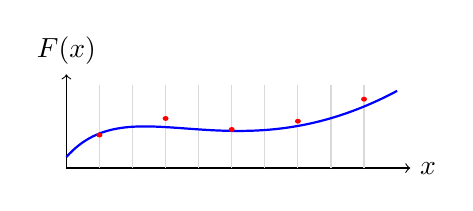
\begin{tikzpicture}[x=0.42cm,y=0.35cm]
 \draw[->] (0,0)--(10.4,0) node[right] {$x$};
 \draw[->] (0,0)--(0,3.4) node[above] {$F(x)$};
 \foreach \x in {1,...,9} {\draw[gray!30] (\x,0)--(\x,3);}
 \draw[blue,thick] (0,0.4) .. controls (2,3.1) and (5,-0.4) .. (10,2.8);
 \foreach \x/\y in {1/1.2,3/1.8,5/1.4,7/1.7,9/2.5}
   \fill[red] (\x,\y) circle (0.09);
\end{tikzpicture}
\end{center}
The next comparison uses Theorem~\ref{thm:32} and Equation~\ref{eq:33}. The proof separates the algebraic estimate from the geometric example. This makes the document useful for edits to prose, formulas, headings and diagrams, while retaining enough ordinary text to exercise paragraph breaking and natural pagination.

\lipsum[18]

\section{A changing estimate: case 035}\label{unit:34}
An observer can return to an earlier part of the document while compilation continues. The relevant statement, equation and hyperlink must still belong to the page actually displayed, including when line wrapping pushes a later theorem across a page boundary.

\lipsum[13-14]
\begin{align}\label{eq:34}
 F_k(x+h)&=F_k(x)+hF_k'(x)+\frac{h^2}{2}F_k''(x)+O(h^3),\\
 \int_0^1 t^k(1-t)\,dt&=\frac{1}{(k+1)(k+2)}.
\end{align}
\begin{theorem}\label{thm:34}
For the finite family in case 35, the normalized error is bounded by $C_k h^2$ whenever $0<h<1$. The constant may depend on $k$ but is independent of the location of the edited paragraph.
\end{theorem}
\begin{proof}
Expand the two terms, collect their first-order contributions, and apply the
triangle inequality. The remaining integral is bounded on the compact interval,
so the asserted estimate follows. This argument also applies after a line break
moves the statement to the next page.
\end{proof}
The next comparison uses Theorem~\ref{thm:33} and Equation~\ref{eq:34}. A local change should remain attached to its source even when surrounding material moves. We compare the displayed argument with the current source version, rather than treating the last compiled page number as a permanent identity.

\lipsum[23]

\section{A changing estimate: case 036}\label{unit:35}
The proof separates the algebraic estimate from the geometric example. This makes the document useful for edits to prose, formulas, headings and diagrams, while retaining enough ordinary text to exercise paragraph breaking and natural pagination.

\lipsum[16-17]
\begin{align}\label{eq:35}
 F_k(x+h)&=F_k(x)+hF_k'(x)+\frac{h^2}{2}F_k''(x)+O(h^3),\\
 \int_0^1 t^k(1-t)\,dt&=\frac{1}{(k+1)(k+2)}.
\end{align}
\begin{theorem}\label{thm:35}
For the finite family in case 36, the normalized error is bounded by $C_k h^2$ whenever $0<h<1$. The constant may depend on $k$ but is independent of the location of the edited paragraph.
\end{theorem}
\begin{proof}
Expand the two terms, collect their first-order contributions, and apply the
triangle inequality. The remaining integral is bounded on the compact interval,
so the asserted estimate follows. This argument also applies after a line break
moves the statement to the next page.
\end{proof}
The next comparison uses Theorem~\ref{thm:34} and Equation~\ref{eq:35}. The construction uses a finite family of examples with different paragraph lengths. Some sentences are short. Others follow the dependence of an estimate on its parameters, introduce a counterexample, and explain why a nearby bound must be reconsidered after an insertion.

\lipsum[3]

\section{A changing estimate: case 037}\label{unit:36}
A local change should remain attached to its source even when surrounding material moves. We compare the displayed argument with the current source version, rather than treating the last compiled page number as a permanent identity.

\lipsum[19-20]
\begin{align}\label{eq:36}
 F_k(x+h)&=F_k(x)+hF_k'(x)+\frac{h^2}{2}F_k''(x)+O(h^3),\\
 \int_0^1 t^k(1-t)\,dt&=\frac{1}{(k+1)(k+2)}.
\end{align}
\begin{lemma}\label{thm:36}
For the finite family in case 37, the normalized error is bounded by $C_k h^2$ whenever $0<h<1$. The constant may depend on $k$ but is independent of the location of the edited paragraph.
\end{lemma}
\begin{proof}
Expand the two terms, collect their first-order contributions, and apply the
triangle inequality. The remaining integral is bounded on the compact interval,
so the asserted estimate follows. This argument also applies after a line break
moves the statement to the next page.
\end{proof}
The next comparison uses Theorem~\ref{thm:35} and Equation~\ref{eq:36}. An observer can return to an earlier part of the document while compilation continues. The relevant statement, equation and hyperlink must still belong to the page actually displayed, including when line wrapping pushes a later theorem across a page boundary.

\lipsum[8]

\section{A changing estimate: case 038}\label{unit:37}
The construction uses a finite family of examples with different paragraph lengths. Some sentences are short. Others follow the dependence of an estimate on its parameters, introduce a counterexample, and explain why a nearby bound must be reconsidered after an insertion.

\lipsum[22-23]
\begin{align}\label{eq:37}
 F_k(x+h)&=F_k(x)+hF_k'(x)+\frac{h^2}{2}F_k''(x)+O(h^3),\\
 \int_0^1 t^k(1-t)\,dt&=\frac{1}{(k+1)(k+2)}.
\end{align}
\begin{theorem}\label{thm:37}
For the finite family in case 38, the normalized error is bounded by $C_k h^2$ whenever $0<h<1$. The constant may depend on $k$ but is independent of the location of the edited paragraph.
\end{theorem}
\begin{proof}
Expand the two terms, collect their first-order contributions, and apply the
triangle inequality. The remaining integral is bounded on the compact interval,
so the asserted estimate follows. This argument also applies after a line break
moves the statement to the next page.
\end{proof}
The next comparison uses Theorem~\ref{thm:36} and Equation~\ref{eq:37}. The proof separates the algebraic estimate from the geometric example. This makes the document useful for edits to prose, formulas, headings and diagrams, while retaining enough ordinary text to exercise paragraph breaking and natural pagination.

\lipsum[13]

\section{A changing estimate: case 039}\label{unit:38}
An observer can return to an earlier part of the document while compilation continues. The relevant statement, equation and hyperlink must still belong to the page actually displayed, including when line wrapping pushes a later theorem across a page boundary.

\lipsum[25-26]
\begin{align}\label{eq:38}
 F_k(x+h)&=F_k(x)+hF_k'(x)+\frac{h^2}{2}F_k''(x)+O(h^3),\\
 \int_0^1 t^k(1-t)\,dt&=\frac{1}{(k+1)(k+2)}.
\end{align}
\begin{theorem}\label{thm:38}
For the finite family in case 39, the normalized error is bounded by $C_k h^2$ whenever $0<h<1$. The constant may depend on $k$ but is independent of the location of the edited paragraph.
\end{theorem}
\begin{proof}
Expand the two terms, collect their first-order contributions, and apply the
triangle inequality. The remaining integral is bounded on the compact interval,
so the asserted estimate follows. This argument also applies after a line break
moves the statement to the next page.
\end{proof}
The next comparison uses Theorem~\ref{thm:37} and Equation~\ref{eq:38}. A local change should remain attached to its source even when surrounding material moves. We compare the displayed argument with the current source version, rather than treating the last compiled page number as a permanent identity.

\lipsum[18]

\section{A changing estimate: case 040}\label{unit:39}
The proof separates the algebraic estimate from the geometric example. This makes the document useful for edits to prose, formulas, headings and diagrams, while retaining enough ordinary text to exercise paragraph breaking and natural pagination.

\lipsum[28-29]
\begin{align}\label{eq:39}
 F_k(x+h)&=F_k(x)+hF_k'(x)+\frac{h^2}{2}F_k''(x)+O(h^3),\\
 \int_0^1 t^k(1-t)\,dt&=\frac{1}{(k+1)(k+2)}.
\end{align}
\begin{lemma}\label{thm:39}
For the finite family in case 40, the normalized error is bounded by $C_k h^2$ whenever $0<h<1$. The constant may depend on $k$ but is independent of the location of the edited paragraph.
\end{lemma}
\begin{proof}
Expand the two terms, collect their first-order contributions, and apply the
triangle inequality. The remaining integral is bounded on the compact interval,
so the asserted estimate follows. This argument also applies after a line break
moves the statement to the next page.
\end{proof}
\begin{center}
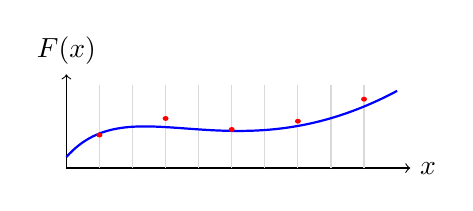
\begin{tikzpicture}[x=0.42cm,y=0.35cm]
 \draw[->] (0,0)--(10.4,0) node[right] {$x$};
 \draw[->] (0,0)--(0,3.4) node[above] {$F(x)$};
 \foreach \x in {1,...,9} {\draw[gray!30] (\x,0)--(\x,3);}
 \draw[blue,thick] (0,0.4) .. controls (2,3.1) and (5,-0.4) .. (10,2.8);
 \foreach \x/\y in {1/1.2,3/1.8,5/1.4,7/1.7,9/2.5}
   \fill[red] (\x,\y) circle (0.09);
\end{tikzpicture}
\end{center}
The next comparison uses Theorem~\ref{thm:38} and Equation~\ref{eq:39}. The construction uses a finite family of examples with different paragraph lengths. Some sentences are short. Others follow the dependence of an estimate on its parameters, introduce a counterexample, and explain why a nearby bound must be reconsidered after an insertion.

\lipsum[23]

\section{A changing estimate: case 041}\label{unit:40}
A local change should remain attached to its source even when surrounding material moves. We compare the displayed argument with the current source version, rather than treating the last compiled page number as a permanent identity.

\lipsum[1-2]
\begin{align}\label{eq:40}
 F_k(x+h)&=F_k(x)+hF_k'(x)+\frac{h^2}{2}F_k''(x)+O(h^3),\\
 \int_0^1 t^k(1-t)\,dt&=\frac{1}{(k+1)(k+2)}.
\end{align}
\begin{theorem}\label{thm:40}
For the finite family in case 41, the normalized error is bounded by $C_k h^2$ whenever $0<h<1$. The constant may depend on $k$ but is independent of the location of the edited paragraph.
\end{theorem}
\begin{proof}
Expand the two terms, collect their first-order contributions, and apply the
triangle inequality. The remaining integral is bounded on the compact interval,
so the asserted estimate follows. This argument also applies after a line break
moves the statement to the next page.
\end{proof}
The next comparison uses Theorem~\ref{thm:39} and Equation~\ref{eq:40}. An observer can return to an earlier part of the document while compilation continues. The relevant statement, equation and hyperlink must still belong to the page actually displayed, including when line wrapping pushes a later theorem across a page boundary.

\lipsum[3]

\section{A changing estimate: case 042}\label{unit:41}
The construction uses a finite family of examples with different paragraph lengths. Some sentences are short. Others follow the dependence of an estimate on its parameters, introduce a counterexample, and explain why a nearby bound must be reconsidered after an insertion.

\lipsum[4-5]
\begin{align}\label{eq:41}
 F_k(x+h)&=F_k(x)+hF_k'(x)+\frac{h^2}{2}F_k''(x)+O(h^3),\\
 \int_0^1 t^k(1-t)\,dt&=\frac{1}{(k+1)(k+2)}.
\end{align}
\begin{theorem}\label{thm:41}
For the finite family in case 42, the normalized error is bounded by $C_k h^2$ whenever $0<h<1$. The constant may depend on $k$ but is independent of the location of the edited paragraph.
\end{theorem}
\begin{proof}
Expand the two terms, collect their first-order contributions, and apply the
triangle inequality. The remaining integral is bounded on the compact interval,
so the asserted estimate follows. This argument also applies after a line break
moves the statement to the next page.
\end{proof}
The next comparison uses Theorem~\ref{thm:40} and Equation~\ref{eq:41}. The proof separates the algebraic estimate from the geometric example. This makes the document useful for edits to prose, formulas, headings and diagrams, while retaining enough ordinary text to exercise paragraph breaking and natural pagination.

\lipsum[8]

\section{A changing estimate: case 043}\label{unit:42}
An observer can return to an earlier part of the document while compilation continues. The relevant statement, equation and hyperlink must still belong to the page actually displayed, including when line wrapping pushes a later theorem across a page boundary.

\lipsum[7-8]
\begin{align}\label{eq:42}
 F_k(x+h)&=F_k(x)+hF_k'(x)+\frac{h^2}{2}F_k''(x)+O(h^3),\\
 \int_0^1 t^k(1-t)\,dt&=\frac{1}{(k+1)(k+2)}.
\end{align}
\begin{lemma}\label{thm:42}
For the finite family in case 43, the normalized error is bounded by $C_k h^2$ whenever $0<h<1$. The constant may depend on $k$ but is independent of the location of the edited paragraph.
\end{lemma}
\begin{proof}
Expand the two terms, collect their first-order contributions, and apply the
triangle inequality. The remaining integral is bounded on the compact interval,
so the asserted estimate follows. This argument also applies after a line break
moves the statement to the next page.
\end{proof}
The next comparison uses Theorem~\ref{thm:41} and Equation~\ref{eq:42}. A local change should remain attached to its source even when surrounding material moves. We compare the displayed argument with the current source version, rather than treating the last compiled page number as a permanent identity.

\lipsum[13]

\section{A changing estimate: case 044}\label{unit:43}
The proof separates the algebraic estimate from the geometric example. This makes the document useful for edits to prose, formulas, headings and diagrams, while retaining enough ordinary text to exercise paragraph breaking and natural pagination.

\lipsum[10-11]
\begin{align}\label{eq:43}
 F_k(x+h)&=F_k(x)+hF_k'(x)+\frac{h^2}{2}F_k''(x)+O(h^3),\\
 \int_0^1 t^k(1-t)\,dt&=\frac{1}{(k+1)(k+2)}.
\end{align}
\begin{theorem}\label{thm:43}
For the finite family in case 44, the normalized error is bounded by $C_k h^2$ whenever $0<h<1$. The constant may depend on $k$ but is independent of the location of the edited paragraph.
\end{theorem}
\begin{proof}
Expand the two terms, collect their first-order contributions, and apply the
triangle inequality. The remaining integral is bounded on the compact interval,
so the asserted estimate follows. This argument also applies after a line break
moves the statement to the next page.
\end{proof}
The next comparison uses Theorem~\ref{thm:42} and Equation~\ref{eq:43}. The construction uses a finite family of examples with different paragraph lengths. Some sentences are short. Others follow the dependence of an estimate on its parameters, introduce a counterexample, and explain why a nearby bound must be reconsidered after an insertion.

\lipsum[18]

\section{A changing estimate: case 045}\label{unit:44}
A local change should remain attached to its source even when surrounding material moves. We compare the displayed argument with the current source version, rather than treating the last compiled page number as a permanent identity.

\lipsum[13-14]
\begin{align}\label{eq:44}
 F_k(x+h)&=F_k(x)+hF_k'(x)+\frac{h^2}{2}F_k''(x)+O(h^3),\\
 \int_0^1 t^k(1-t)\,dt&=\frac{1}{(k+1)(k+2)}.
\end{align}
\begin{theorem}\label{thm:44}
For the finite family in case 45, the normalized error is bounded by $C_k h^2$ whenever $0<h<1$. The constant may depend on $k$ but is independent of the location of the edited paragraph.
\end{theorem}
\begin{proof}
Expand the two terms, collect their first-order contributions, and apply the
triangle inequality. The remaining integral is bounded on the compact interval,
so the asserted estimate follows. This argument also applies after a line break
moves the statement to the next page.
\end{proof}
The next comparison uses Theorem~\ref{thm:43} and Equation~\ref{eq:44}. An observer can return to an earlier part of the document while compilation continues. The relevant statement, equation and hyperlink must still belong to the page actually displayed, including when line wrapping pushes a later theorem across a page boundary.

\lipsum[23]

\section{A changing estimate: case 046}\label{unit:45}
The construction uses a finite family of examples with different paragraph lengths. Some sentences are short. Others follow the dependence of an estimate on its parameters, introduce a counterexample, and explain why a nearby bound must be reconsidered after an insertion.

\lipsum[16-17]
\begin{align}\label{eq:45}
 F_k(x+h)&=F_k(x)+hF_k'(x)+\frac{h^2}{2}F_k''(x)+O(h^3),\\
 \int_0^1 t^k(1-t)\,dt&=\frac{1}{(k+1)(k+2)}.
\end{align}
\begin{lemma}\label{thm:45}
For the finite family in case 46, the normalized error is bounded by $C_k h^2$ whenever $0<h<1$. The constant may depend on $k$ but is independent of the location of the edited paragraph.
\end{lemma}
\begin{proof}
Expand the two terms, collect their first-order contributions, and apply the
triangle inequality. The remaining integral is bounded on the compact interval,
so the asserted estimate follows. This argument also applies after a line break
moves the statement to the next page.
\end{proof}
\begin{center}
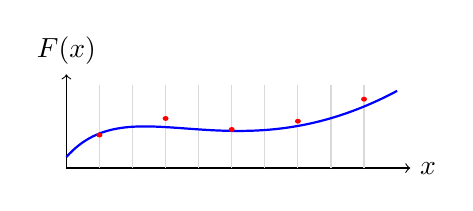
\begin{tikzpicture}[x=0.42cm,y=0.35cm]
 \draw[->] (0,0)--(10.4,0) node[right] {$x$};
 \draw[->] (0,0)--(0,3.4) node[above] {$F(x)$};
 \foreach \x in {1,...,9} {\draw[gray!30] (\x,0)--(\x,3);}
 \draw[blue,thick] (0,0.4) .. controls (2,3.1) and (5,-0.4) .. (10,2.8);
 \foreach \x/\y in {1/1.2,3/1.8,5/1.4,7/1.7,9/2.5}
   \fill[red] (\x,\y) circle (0.09);
\end{tikzpicture}
\end{center}
The next comparison uses Theorem~\ref{thm:44} and Equation~\ref{eq:45}. The proof separates the algebraic estimate from the geometric example. This makes the document useful for edits to prose, formulas, headings and diagrams, while retaining enough ordinary text to exercise paragraph breaking and natural pagination.

\lipsum[3]

\section{A changing estimate: case 047}\label{unit:46}
An observer can return to an earlier part of the document while compilation continues. The relevant statement, equation and hyperlink must still belong to the page actually displayed, including when line wrapping pushes a later theorem across a page boundary.

\lipsum[19-20]
\begin{align}\label{eq:46}
 F_k(x+h)&=F_k(x)+hF_k'(x)+\frac{h^2}{2}F_k''(x)+O(h^3),\\
 \int_0^1 t^k(1-t)\,dt&=\frac{1}{(k+1)(k+2)}.
\end{align}
\begin{theorem}\label{thm:46}
For the finite family in case 47, the normalized error is bounded by $C_k h^2$ whenever $0<h<1$. The constant may depend on $k$ but is independent of the location of the edited paragraph.
\end{theorem}
\begin{proof}
Expand the two terms, collect their first-order contributions, and apply the
triangle inequality. The remaining integral is bounded on the compact interval,
so the asserted estimate follows. This argument also applies after a line break
moves the statement to the next page.
\end{proof}
The next comparison uses Theorem~\ref{thm:45} and Equation~\ref{eq:46}. A local change should remain attached to its source even when surrounding material moves. We compare the displayed argument with the current source version, rather than treating the last compiled page number as a permanent identity.

\lipsum[8]

\section{A changing estimate: case 048}\label{unit:47}
The proof separates the algebraic estimate from the geometric example. This makes the document useful for edits to prose, formulas, headings and diagrams, while retaining enough ordinary text to exercise paragraph breaking and natural pagination.

\lipsum[22-23]
\begin{align}\label{eq:47}
 F_k(x+h)&=F_k(x)+hF_k'(x)+\frac{h^2}{2}F_k''(x)+O(h^3),\\
 \int_0^1 t^k(1-t)\,dt&=\frac{1}{(k+1)(k+2)}.
\end{align}
\begin{theorem}\label{thm:47}
For the finite family in case 48, the normalized error is bounded by $C_k h^2$ whenever $0<h<1$. The constant may depend on $k$ but is independent of the location of the edited paragraph.
\end{theorem}
\begin{proof}
Expand the two terms, collect their first-order contributions, and apply the
triangle inequality. The remaining integral is bounded on the compact interval,
so the asserted estimate follows. This argument also applies after a line break
moves the statement to the next page.
\end{proof}
The next comparison uses Theorem~\ref{thm:46} and Equation~\ref{eq:47}. The construction uses a finite family of examples with different paragraph lengths. Some sentences are short. Others follow the dependence of an estimate on its parameters, introduce a counterexample, and explain why a nearby bound must be reconsidered after an insertion.

\lipsum[13]

\section{A changing estimate: case 049}\label{unit:48}
A local change should remain attached to its source even when surrounding material moves. We compare the displayed argument with the current source version, rather than treating the last compiled page number as a permanent identity.

\lipsum[25-26]
\begin{align}\label{eq:48}
 F_k(x+h)&=F_k(x)+hF_k'(x)+\frac{h^2}{2}F_k''(x)+O(h^3),\\
 \int_0^1 t^k(1-t)\,dt&=\frac{1}{(k+1)(k+2)}.
\end{align}
\begin{lemma}\label{thm:48}
For the finite family in case 49, the normalized error is bounded by $C_k h^2$ whenever $0<h<1$. The constant may depend on $k$ but is independent of the location of the edited paragraph.
\end{lemma}
\begin{proof}
Expand the two terms, collect their first-order contributions, and apply the
triangle inequality. The remaining integral is bounded on the compact interval,
so the asserted estimate follows. This argument also applies after a line break
moves the statement to the next page.
\end{proof}
The next comparison uses Theorem~\ref{thm:47} and Equation~\ref{eq:48}. An observer can return to an earlier part of the document while compilation continues. The relevant statement, equation and hyperlink must still belong to the page actually displayed, including when line wrapping pushes a later theorem across a page boundary.

\lipsum[18]

\section{A changing estimate: case 050}\label{unit:49}
The construction uses a finite family of examples with different paragraph lengths. Some sentences are short. Others follow the dependence of an estimate on its parameters, introduce a counterexample, and explain why a nearby bound must be reconsidered after an insertion.

\lipsum[28-29]
\begin{align}\label{eq:49}
 F_k(x+h)&=F_k(x)+hF_k'(x)+\frac{h^2}{2}F_k''(x)+O(h^3),\\
 \int_0^1 t^k(1-t)\,dt&=\frac{1}{(k+1)(k+2)}.
\end{align}
\begin{theorem}\label{thm:49}
For the finite family in case 50, the normalized error is bounded by $C_k h^2$ whenever $0<h<1$. The constant may depend on $k$ but is independent of the location of the edited paragraph.
\end{theorem}
\begin{proof}
Expand the two terms, collect their first-order contributions, and apply the
triangle inequality. The remaining integral is bounded on the compact interval,
so the asserted estimate follows. This argument also applies after a line break
moves the statement to the next page.
\end{proof}
The next comparison uses Theorem~\ref{thm:48} and Equation~\ref{eq:49}. The proof separates the algebraic estimate from the geometric example. This makes the document useful for edits to prose, formulas, headings and diagrams, while retaining enough ordinary text to exercise paragraph breaking and natural pagination.

\lipsum[23]

\section{A changing estimate: case 051}\label{unit:50}
An observer can return to an earlier part of the document while compilation continues. The relevant statement, equation and hyperlink must still belong to the page actually displayed, including when line wrapping pushes a later theorem across a page boundary.

\lipsum[1-2]
\begin{align}\label{eq:50}
 F_k(x+h)&=F_k(x)+hF_k'(x)+\frac{h^2}{2}F_k''(x)+O(h^3),\\
 \int_0^1 t^k(1-t)\,dt&=\frac{1}{(k+1)(k+2)}.
\end{align}
\begin{theorem}\label{thm:50}
For the finite family in case 51, the normalized error is bounded by $C_k h^2$ whenever $0<h<1$. The constant may depend on $k$ but is independent of the location of the edited paragraph.
\end{theorem}
\begin{proof}
Expand the two terms, collect their first-order contributions, and apply the
triangle inequality. The remaining integral is bounded on the compact interval,
so the asserted estimate follows. This argument also applies after a line break
moves the statement to the next page.
\end{proof}
The next comparison uses Theorem~\ref{thm:49} and Equation~\ref{eq:50}. A local change should remain attached to its source even when surrounding material moves. We compare the displayed argument with the current source version, rather than treating the last compiled page number as a permanent identity.

\lipsum[3]

\section{A changing estimate: case 052}\label{unit:51}
The proof separates the algebraic estimate from the geometric example. This makes the document useful for edits to prose, formulas, headings and diagrams, while retaining enough ordinary text to exercise paragraph breaking and natural pagination.

\lipsum[4-5]
\begin{align}\label{eq:51}
 F_k(x+h)&=F_k(x)+hF_k'(x)+\frac{h^2}{2}F_k''(x)+O(h^3),\\
 \int_0^1 t^k(1-t)\,dt&=\frac{1}{(k+1)(k+2)}.
\end{align}
\begin{lemma}\label{thm:51}
For the finite family in case 52, the normalized error is bounded by $C_k h^2$ whenever $0<h<1$. The constant may depend on $k$ but is independent of the location of the edited paragraph.
\end{lemma}
\begin{proof}
Expand the two terms, collect their first-order contributions, and apply the
triangle inequality. The remaining integral is bounded on the compact interval,
so the asserted estimate follows. This argument also applies after a line break
moves the statement to the next page.
\end{proof}
\begin{center}
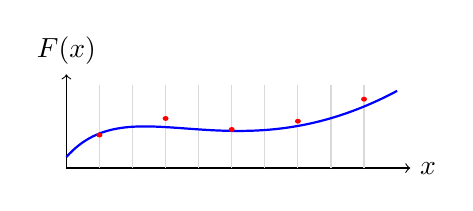
\begin{tikzpicture}[x=0.42cm,y=0.35cm]
 \draw[->] (0,0)--(10.4,0) node[right] {$x$};
 \draw[->] (0,0)--(0,3.4) node[above] {$F(x)$};
 \foreach \x in {1,...,9} {\draw[gray!30] (\x,0)--(\x,3);}
 \draw[blue,thick] (0,0.4) .. controls (2,3.1) and (5,-0.4) .. (10,2.8);
 \foreach \x/\y in {1/1.2,3/1.8,5/1.4,7/1.7,9/2.5}
   \fill[red] (\x,\y) circle (0.09);
\end{tikzpicture}
\end{center}
The next comparison uses Theorem~\ref{thm:50} and Equation~\ref{eq:51}. The construction uses a finite family of examples with different paragraph lengths. Some sentences are short. Others follow the dependence of an estimate on its parameters, introduce a counterexample, and explain why a nearby bound must be reconsidered after an insertion.

\lipsum[8]

\section{A changing estimate: case 053}\label{unit:52}
A local change should remain attached to its source even when surrounding material moves. We compare the displayed argument with the current source version, rather than treating the last compiled page number as a permanent identity.

\lipsum[7-8]
\begin{align}\label{eq:52}
 F_k(x+h)&=F_k(x)+hF_k'(x)+\frac{h^2}{2}F_k''(x)+O(h^3),\\
 \int_0^1 t^k(1-t)\,dt&=\frac{1}{(k+1)(k+2)}.
\end{align}
\begin{theorem}\label{thm:52}
For the finite family in case 53, the normalized error is bounded by $C_k h^2$ whenever $0<h<1$. The constant may depend on $k$ but is independent of the location of the edited paragraph.
\end{theorem}
\begin{proof}
Expand the two terms, collect their first-order contributions, and apply the
triangle inequality. The remaining integral is bounded on the compact interval,
so the asserted estimate follows. This argument also applies after a line break
moves the statement to the next page.
\end{proof}
The next comparison uses Theorem~\ref{thm:51} and Equation~\ref{eq:52}. An observer can return to an earlier part of the document while compilation continues. The relevant statement, equation and hyperlink must still belong to the page actually displayed, including when line wrapping pushes a later theorem across a page boundary.

\lipsum[13]

\section{A changing estimate: case 054}\label{unit:53}
The construction uses a finite family of examples with different paragraph lengths. Some sentences are short. Others follow the dependence of an estimate on its parameters, introduce a counterexample, and explain why a nearby bound must be reconsidered after an insertion.

\lipsum[10-11]
\begin{align}\label{eq:53}
 F_k(x+h)&=F_k(x)+hF_k'(x)+\frac{h^2}{2}F_k''(x)+O(h^3),\\
 \int_0^1 t^k(1-t)\,dt&=\frac{1}{(k+1)(k+2)}.
\end{align}
\begin{theorem}\label{thm:53}
For the finite family in case 54, the normalized error is bounded by $C_k h^2$ whenever $0<h<1$. The constant may depend on $k$ but is independent of the location of the edited paragraph.
\end{theorem}
\begin{proof}
Expand the two terms, collect their first-order contributions, and apply the
triangle inequality. The remaining integral is bounded on the compact interval,
so the asserted estimate follows. This argument also applies after a line break
moves the statement to the next page.
\end{proof}
The next comparison uses Theorem~\ref{thm:52} and Equation~\ref{eq:53}. The proof separates the algebraic estimate from the geometric example. This makes the document useful for edits to prose, formulas, headings and diagrams, while retaining enough ordinary text to exercise paragraph breaking and natural pagination.

\lipsum[18]

\section{A changing estimate: case 055}\label{unit:54}
An observer can return to an earlier part of the document while compilation continues. The relevant statement, equation and hyperlink must still belong to the page actually displayed, including when line wrapping pushes a later theorem across a page boundary.

\lipsum[13-14]
\begin{align}\label{eq:54}
 F_k(x+h)&=F_k(x)+hF_k'(x)+\frac{h^2}{2}F_k''(x)+O(h^3),\\
 \int_0^1 t^k(1-t)\,dt&=\frac{1}{(k+1)(k+2)}.
\end{align}
\begin{lemma}\label{thm:54}
For the finite family in case 55, the normalized error is bounded by $C_k h^2$ whenever $0<h<1$. The constant may depend on $k$ but is independent of the location of the edited paragraph.
\end{lemma}
\begin{proof}
Expand the two terms, collect their first-order contributions, and apply the
triangle inequality. The remaining integral is bounded on the compact interval,
so the asserted estimate follows. This argument also applies after a line break
moves the statement to the next page.
\end{proof}
The next comparison uses Theorem~\ref{thm:53} and Equation~\ref{eq:54}. A local change should remain attached to its source even when surrounding material moves. We compare the displayed argument with the current source version, rather than treating the last compiled page number as a permanent identity.

\lipsum[23]

\section{A changing estimate: case 056}\label{unit:55}
The proof separates the algebraic estimate from the geometric example. This makes the document useful for edits to prose, formulas, headings and diagrams, while retaining enough ordinary text to exercise paragraph breaking and natural pagination.

\lipsum[16-17]
\begin{align}\label{eq:55}
 F_k(x+h)&=F_k(x)+hF_k'(x)+\frac{h^2}{2}F_k''(x)+O(h^3),\\
 \int_0^1 t^k(1-t)\,dt&=\frac{1}{(k+1)(k+2)}.
\end{align}
\begin{theorem}\label{thm:55}
For the finite family in case 56, the normalized error is bounded by $C_k h^2$ whenever $0<h<1$. The constant may depend on $k$ but is independent of the location of the edited paragraph.
\end{theorem}
\begin{proof}
Expand the two terms, collect their first-order contributions, and apply the
triangle inequality. The remaining integral is bounded on the compact interval,
so the asserted estimate follows. This argument also applies after a line break
moves the statement to the next page.
\end{proof}
The next comparison uses Theorem~\ref{thm:54} and Equation~\ref{eq:55}. The construction uses a finite family of examples with different paragraph lengths. Some sentences are short. Others follow the dependence of an estimate on its parameters, introduce a counterexample, and explain why a nearby bound must be reconsidered after an insertion.

\lipsum[3]

\section{A changing estimate: case 057}\label{unit:56}
A local change should remain attached to its source even when surrounding material moves. We compare the displayed argument with the current source version, rather than treating the last compiled page number as a permanent identity.

\lipsum[19-20]
\begin{align}\label{eq:56}
 F_k(x+h)&=F_k(x)+hF_k'(x)+\frac{h^2}{2}F_k''(x)+O(h^3),\\
 \int_0^1 t^k(1-t)\,dt&=\frac{1}{(k+1)(k+2)}.
\end{align}
\begin{theorem}\label{thm:56}
For the finite family in case 57, the normalized error is bounded by $C_k h^2$ whenever $0<h<1$. The constant may depend on $k$ but is independent of the location of the edited paragraph.
\end{theorem}
\begin{proof}
Expand the two terms, collect their first-order contributions, and apply the
triangle inequality. The remaining integral is bounded on the compact interval,
so the asserted estimate follows. This argument also applies after a line break
moves the statement to the next page.
\end{proof}
The next comparison uses Theorem~\ref{thm:55} and Equation~\ref{eq:56}. An observer can return to an earlier part of the document while compilation continues. The relevant statement, equation and hyperlink must still belong to the page actually displayed, including when line wrapping pushes a later theorem across a page boundary.

\lipsum[8]

\section{A changing estimate: case 058}\label{unit:57}
The construction uses a finite family of examples with different paragraph lengths. Some sentences are short. Others follow the dependence of an estimate on its parameters, introduce a counterexample, and explain why a nearby bound must be reconsidered after an insertion.

\lipsum[22-23]
\begin{align}\label{eq:57}
 F_k(x+h)&=F_k(x)+hF_k'(x)+\frac{h^2}{2}F_k''(x)+O(h^3),\\
 \int_0^1 t^k(1-t)\,dt&=\frac{1}{(k+1)(k+2)}.
\end{align}
\begin{lemma}\label{thm:57}
For the finite family in case 58, the normalized error is bounded by $C_k h^2$ whenever $0<h<1$. The constant may depend on $k$ but is independent of the location of the edited paragraph.
\end{lemma}
\begin{proof}
Expand the two terms, collect their first-order contributions, and apply the
triangle inequality. The remaining integral is bounded on the compact interval,
so the asserted estimate follows. This argument also applies after a line break
moves the statement to the next page.
\end{proof}
\begin{center}
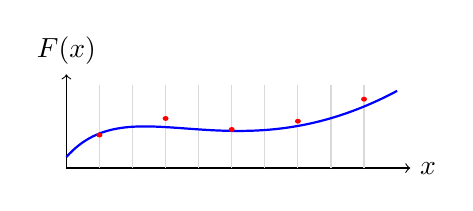
\begin{tikzpicture}[x=0.42cm,y=0.35cm]
 \draw[->] (0,0)--(10.4,0) node[right] {$x$};
 \draw[->] (0,0)--(0,3.4) node[above] {$F(x)$};
 \foreach \x in {1,...,9} {\draw[gray!30] (\x,0)--(\x,3);}
 \draw[blue,thick] (0,0.4) .. controls (2,3.1) and (5,-0.4) .. (10,2.8);
 \foreach \x/\y in {1/1.2,3/1.8,5/1.4,7/1.7,9/2.5}
   \fill[red] (\x,\y) circle (0.09);
\end{tikzpicture}
\end{center}
The next comparison uses Theorem~\ref{thm:56} and Equation~\ref{eq:57}. The proof separates the algebraic estimate from the geometric example. This makes the document useful for edits to prose, formulas, headings and diagrams, while retaining enough ordinary text to exercise paragraph breaking and natural pagination.

\lipsum[13]

\section{A changing estimate: case 059}\label{unit:58}
An observer can return to an earlier part of the document while compilation continues. The relevant statement, equation and hyperlink must still belong to the page actually displayed, including when line wrapping pushes a later theorem across a page boundary.

\lipsum[25-26]
\begin{align}\label{eq:58}
 F_k(x+h)&=F_k(x)+hF_k'(x)+\frac{h^2}{2}F_k''(x)+O(h^3),\\
 \int_0^1 t^k(1-t)\,dt&=\frac{1}{(k+1)(k+2)}.
\end{align}
\begin{theorem}\label{thm:58}
For the finite family in case 59, the normalized error is bounded by $C_k h^2$ whenever $0<h<1$. The constant may depend on $k$ but is independent of the location of the edited paragraph.
\end{theorem}
\begin{proof}
Expand the two terms, collect their first-order contributions, and apply the
triangle inequality. The remaining integral is bounded on the compact interval,
so the asserted estimate follows. This argument also applies after a line break
moves the statement to the next page.
\end{proof}
The next comparison uses Theorem~\ref{thm:57} and Equation~\ref{eq:58}. A local change should remain attached to its source even when surrounding material moves. We compare the displayed argument with the current source version, rather than treating the last compiled page number as a permanent identity.

\lipsum[18]

\section{A changing estimate: case 060}\label{unit:59}
The proof separates the algebraic estimate from the geometric example. This makes the document useful for edits to prose, formulas, headings and diagrams, while retaining enough ordinary text to exercise paragraph breaking and natural pagination.

\lipsum[28-29]
\begin{align}\label{eq:59}
 F_k(x+h)&=F_k(x)+hF_k'(x)+\frac{h^2}{2}F_k''(x)+O(h^3),\\
 \int_0^1 t^k(1-t)\,dt&=\frac{1}{(k+1)(k+2)}.
\end{align}
\begin{theorem}\label{thm:59}
For the finite family in case 60, the normalized error is bounded by $C_k h^2$ whenever $0<h<1$. The constant may depend on $k$ but is independent of the location of the edited paragraph.
\end{theorem}
\begin{proof}
Expand the two terms, collect their first-order contributions, and apply the
triangle inequality. The remaining integral is bounded on the compact interval,
so the asserted estimate follows. This argument also applies after a line break
moves the statement to the next page.
\end{proof}
The next comparison uses Theorem~\ref{thm:58} and Equation~\ref{eq:59}. The construction uses a finite family of examples with different paragraph lengths. Some sentences are short. Others follow the dependence of an estimate on its parameters, introduce a counterexample, and explain why a nearby bound must be reconsidered after an insertion.

\lipsum[23]

\section{A changing estimate: case 061}\label{unit:60}
A local change should remain attached to its source even when surrounding material moves. We compare the displayed argument with the current source version, rather than treating the last compiled page number as a permanent identity.

\lipsum[1-2]
\begin{align}\label{eq:60}
 F_k(x+h)&=F_k(x)+hF_k'(x)+\frac{h^2}{2}F_k''(x)+O(h^3),\\
 \int_0^1 t^k(1-t)\,dt&=\frac{1}{(k+1)(k+2)}.
\end{align}
\begin{lemma}\label{thm:60}
For the finite family in case 61, the normalized error is bounded by $C_k h^2$ whenever $0<h<1$. The constant may depend on $k$ but is independent of the location of the edited paragraph.
\end{lemma}
\begin{proof}
Expand the two terms, collect their first-order contributions, and apply the
triangle inequality. The remaining integral is bounded on the compact interval,
so the asserted estimate follows. This argument also applies after a line break
moves the statement to the next page.
\end{proof}
The next comparison uses Theorem~\ref{thm:59} and Equation~\ref{eq:60}. An observer can return to an earlier part of the document while compilation continues. The relevant statement, equation and hyperlink must still belong to the page actually displayed, including when line wrapping pushes a later theorem across a page boundary.

\lipsum[3]

\section{A changing estimate: case 062}\label{unit:61}
The construction uses a finite family of examples with different paragraph lengths. Some sentences are short. Others follow the dependence of an estimate on its parameters, introduce a counterexample, and explain why a nearby bound must be reconsidered after an insertion.

\lipsum[4-5]
\begin{align}\label{eq:61}
 F_k(x+h)&=F_k(x)+hF_k'(x)+\frac{h^2}{2}F_k''(x)+O(h^3),\\
 \int_0^1 t^k(1-t)\,dt&=\frac{1}{(k+1)(k+2)}.
\end{align}
\begin{theorem}\label{thm:61}
For the finite family in case 62, the normalized error is bounded by $C_k h^2$ whenever $0<h<1$. The constant may depend on $k$ but is independent of the location of the edited paragraph.
\end{theorem}
\begin{proof}
Expand the two terms, collect their first-order contributions, and apply the
triangle inequality. The remaining integral is bounded on the compact interval,
so the asserted estimate follows. This argument also applies after a line break
moves the statement to the next page.
\end{proof}
The next comparison uses Theorem~\ref{thm:60} and Equation~\ref{eq:61}. The proof separates the algebraic estimate from the geometric example. This makes the document useful for edits to prose, formulas, headings and diagrams, while retaining enough ordinary text to exercise paragraph breaking and natural pagination.

\lipsum[8]

\section{A changing estimate: case 063}\label{unit:62}
An observer can return to an earlier part of the document while compilation continues. The relevant statement, equation and hyperlink must still belong to the page actually displayed, including when line wrapping pushes a later theorem across a page boundary.

\lipsum[7-8]
\begin{align}\label{eq:62}
 F_k(x+h)&=F_k(x)+hF_k'(x)+\frac{h^2}{2}F_k''(x)+O(h^3),\\
 \int_0^1 t^k(1-t)\,dt&=\frac{1}{(k+1)(k+2)}.
\end{align}
\begin{theorem}\label{thm:62}
For the finite family in case 63, the normalized error is bounded by $C_k h^2$ whenever $0<h<1$. The constant may depend on $k$ but is independent of the location of the edited paragraph.
\end{theorem}
\begin{proof}
Expand the two terms, collect their first-order contributions, and apply the
triangle inequality. The remaining integral is bounded on the compact interval,
so the asserted estimate follows. This argument also applies after a line break
moves the statement to the next page.
\end{proof}
The next comparison uses Theorem~\ref{thm:61} and Equation~\ref{eq:62}. A local change should remain attached to its source even when surrounding material moves. We compare the displayed argument with the current source version, rather than treating the last compiled page number as a permanent identity.

\lipsum[13]

\section{A changing estimate: case 064}\label{unit:63}
The proof separates the algebraic estimate from the geometric example. This makes the document useful for edits to prose, formulas, headings and diagrams, while retaining enough ordinary text to exercise paragraph breaking and natural pagination.

\lipsum[10-11]
\begin{align}\label{eq:63}
 F_k(x+h)&=F_k(x)+hF_k'(x)+\frac{h^2}{2}F_k''(x)+O(h^3),\\
 \int_0^1 t^k(1-t)\,dt&=\frac{1}{(k+1)(k+2)}.
\end{align}
\begin{lemma}\label{thm:63}
For the finite family in case 64, the normalized error is bounded by $C_k h^2$ whenever $0<h<1$. The constant may depend on $k$ but is independent of the location of the edited paragraph.
\end{lemma}
\begin{proof}
Expand the two terms, collect their first-order contributions, and apply the
triangle inequality. The remaining integral is bounded on the compact interval,
so the asserted estimate follows. This argument also applies after a line break
moves the statement to the next page.
\end{proof}
\begin{center}
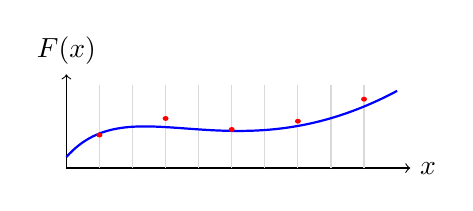
\begin{tikzpicture}[x=0.42cm,y=0.35cm]
 \draw[->] (0,0)--(10.4,0) node[right] {$x$};
 \draw[->] (0,0)--(0,3.4) node[above] {$F(x)$};
 \foreach \x in {1,...,9} {\draw[gray!30] (\x,0)--(\x,3);}
 \draw[blue,thick] (0,0.4) .. controls (2,3.1) and (5,-0.4) .. (10,2.8);
 \foreach \x/\y in {1/1.2,3/1.8,5/1.4,7/1.7,9/2.5}
   \fill[red] (\x,\y) circle (0.09);
\end{tikzpicture}
\end{center}
The next comparison uses Theorem~\ref{thm:62} and Equation~\ref{eq:63}. The construction uses a finite family of examples with different paragraph lengths. Some sentences are short. Others follow the dependence of an estimate on its parameters, introduce a counterexample, and explain why a nearby bound must be reconsidered after an insertion.

\lipsum[18]

\section{A changing estimate: case 065}\label{unit:64}
A local change should remain attached to its source even when surrounding material moves. We compare the displayed argument with the current source version, rather than treating the last compiled page number as a permanent identity.

\lipsum[13-14]
\begin{align}\label{eq:64}
 F_k(x+h)&=F_k(x)+hF_k'(x)+\frac{h^2}{2}F_k''(x)+O(h^3),\\
 \int_0^1 t^k(1-t)\,dt&=\frac{1}{(k+1)(k+2)}.
\end{align}
\begin{theorem}\label{thm:64}
For the finite family in case 65, the normalized error is bounded by $C_k h^2$ whenever $0<h<1$. The constant may depend on $k$ but is independent of the location of the edited paragraph.
\end{theorem}
\begin{proof}
Expand the two terms, collect their first-order contributions, and apply the
triangle inequality. The remaining integral is bounded on the compact interval,
so the asserted estimate follows. This argument also applies after a line break
moves the statement to the next page.
\end{proof}
The next comparison uses Theorem~\ref{thm:63} and Equation~\ref{eq:64}. An observer can return to an earlier part of the document while compilation continues. The relevant statement, equation and hyperlink must still belong to the page actually displayed, including when line wrapping pushes a later theorem across a page boundary.

\lipsum[23]

\section{A changing estimate: case 066}\label{unit:65}
The construction uses a finite family of examples with different paragraph lengths. Some sentences are short. Others follow the dependence of an estimate on its parameters, introduce a counterexample, and explain why a nearby bound must be reconsidered after an insertion.

\lipsum[16-17]
\begin{align}\label{eq:65}
 F_k(x+h)&=F_k(x)+hF_k'(x)+\frac{h^2}{2}F_k''(x)+O(h^3),\\
 \int_0^1 t^k(1-t)\,dt&=\frac{1}{(k+1)(k+2)}.
\end{align}
\begin{theorem}\label{thm:65}
For the finite family in case 66, the normalized error is bounded by $C_k h^2$ whenever $0<h<1$. The constant may depend on $k$ but is independent of the location of the edited paragraph.
\end{theorem}
\begin{proof}
Expand the two terms, collect their first-order contributions, and apply the
triangle inequality. The remaining integral is bounded on the compact interval,
so the asserted estimate follows. This argument also applies after a line break
moves the statement to the next page.
\end{proof}
The next comparison uses Theorem~\ref{thm:64} and Equation~\ref{eq:65}. The proof separates the algebraic estimate from the geometric example. This makes the document useful for edits to prose, formulas, headings and diagrams, while retaining enough ordinary text to exercise paragraph breaking and natural pagination.

\lipsum[3]

\section{A changing estimate: case 067}\label{unit:66}
An observer can return to an earlier part of the document while compilation continues. The relevant statement, equation and hyperlink must still belong to the page actually displayed, including when line wrapping pushes a later theorem across a page boundary.

\lipsum[19-20]
\begin{align}\label{eq:66}
 F_k(x+h)&=F_k(x)+hF_k'(x)+\frac{h^2}{2}F_k''(x)+O(h^3),\\
 \int_0^1 t^k(1-t)\,dt&=\frac{1}{(k+1)(k+2)}.
\end{align}
\begin{lemma}\label{thm:66}
For the finite family in case 67, the normalized error is bounded by $C_k h^2$ whenever $0<h<1$. The constant may depend on $k$ but is independent of the location of the edited paragraph.
\end{lemma}
\begin{proof}
Expand the two terms, collect their first-order contributions, and apply the
triangle inequality. The remaining integral is bounded on the compact interval,
so the asserted estimate follows. This argument also applies after a line break
moves the statement to the next page.
\end{proof}
The next comparison uses Theorem~\ref{thm:65} and Equation~\ref{eq:66}. A local change should remain attached to its source even when surrounding material moves. We compare the displayed argument with the current source version, rather than treating the last compiled page number as a permanent identity.

\lipsum[8]

\section{A changing estimate: case 068}\label{unit:67}
The proof separates the algebraic estimate from the geometric example. This makes the document useful for edits to prose, formulas, headings and diagrams, while retaining enough ordinary text to exercise paragraph breaking and natural pagination.

\lipsum[22-23]
\begin{align}\label{eq:67}
 F_k(x+h)&=F_k(x)+hF_k'(x)+\frac{h^2}{2}F_k''(x)+O(h^3),\\
 \int_0^1 t^k(1-t)\,dt&=\frac{1}{(k+1)(k+2)}.
\end{align}
\begin{theorem}\label{thm:67}
For the finite family in case 68, the normalized error is bounded by $C_k h^2$ whenever $0<h<1$. The constant may depend on $k$ but is independent of the location of the edited paragraph.
\end{theorem}
\begin{proof}
Expand the two terms, collect their first-order contributions, and apply the
triangle inequality. The remaining integral is bounded on the compact interval,
so the asserted estimate follows. This argument also applies after a line break
moves the statement to the next page.
\end{proof}
The next comparison uses Theorem~\ref{thm:66} and Equation~\ref{eq:67}. The construction uses a finite family of examples with different paragraph lengths. Some sentences are short. Others follow the dependence of an estimate on its parameters, introduce a counterexample, and explain why a nearby bound must be reconsidered after an insertion.

\lipsum[13]

\section{A changing estimate: case 069}\label{unit:68}
A local change should remain attached to its source even when surrounding material moves. We compare the displayed argument with the current source version, rather than treating the last compiled page number as a permanent identity.

\lipsum[25-26]
\begin{align}\label{eq:68}
 F_k(x+h)&=F_k(x)+hF_k'(x)+\frac{h^2}{2}F_k''(x)+O(h^3),\\
 \int_0^1 t^k(1-t)\,dt&=\frac{1}{(k+1)(k+2)}.
\end{align}
\begin{theorem}\label{thm:68}
For the finite family in case 69, the normalized error is bounded by $C_k h^2$ whenever $0<h<1$. The constant may depend on $k$ but is independent of the location of the edited paragraph.
\end{theorem}
\begin{proof}
Expand the two terms, collect their first-order contributions, and apply the
triangle inequality. The remaining integral is bounded on the compact interval,
so the asserted estimate follows. This argument also applies after a line break
moves the statement to the next page.
\end{proof}
The next comparison uses Theorem~\ref{thm:67} and Equation~\ref{eq:68}. An observer can return to an earlier part of the document while compilation continues. The relevant statement, equation and hyperlink must still belong to the page actually displayed, including when line wrapping pushes a later theorem across a page boundary.

\lipsum[18]

\section{A changing estimate: case 070}\label{unit:69}
The construction uses a finite family of examples with different paragraph lengths. Some sentences are short. Others follow the dependence of an estimate on its parameters, introduce a counterexample, and explain why a nearby bound must be reconsidered after an insertion.

\lipsum[28-29]
\begin{align}\label{eq:69}
 F_k(x+h)&=F_k(x)+hF_k'(x)+\frac{h^2}{2}F_k''(x)+O(h^3),\\
 \int_0^1 t^k(1-t)\,dt&=\frac{1}{(k+1)(k+2)}.
\end{align}
\begin{lemma}\label{thm:69}
For the finite family in case 70, the normalized error is bounded by $C_k h^2$ whenever $0<h<1$. The constant may depend on $k$ but is independent of the location of the edited paragraph.
\end{lemma}
\begin{proof}
Expand the two terms, collect their first-order contributions, and apply the
triangle inequality. The remaining integral is bounded on the compact interval,
so the asserted estimate follows. This argument also applies after a line break
moves the statement to the next page.
\end{proof}
\begin{center}
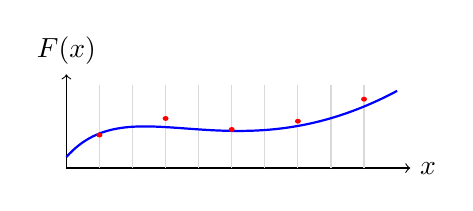
\begin{tikzpicture}[x=0.42cm,y=0.35cm]
 \draw[->] (0,0)--(10.4,0) node[right] {$x$};
 \draw[->] (0,0)--(0,3.4) node[above] {$F(x)$};
 \foreach \x in {1,...,9} {\draw[gray!30] (\x,0)--(\x,3);}
 \draw[blue,thick] (0,0.4) .. controls (2,3.1) and (5,-0.4) .. (10,2.8);
 \foreach \x/\y in {1/1.2,3/1.8,5/1.4,7/1.7,9/2.5}
   \fill[red] (\x,\y) circle (0.09);
\end{tikzpicture}
\end{center}
The next comparison uses Theorem~\ref{thm:68} and Equation~\ref{eq:69}. The proof separates the algebraic estimate from the geometric example. This makes the document useful for edits to prose, formulas, headings and diagrams, while retaining enough ordinary text to exercise paragraph breaking and natural pagination.

\lipsum[23]

\section{A changing estimate: case 071}\label{unit:70}
An observer can return to an earlier part of the document while compilation continues. The relevant statement, equation and hyperlink must still belong to the page actually displayed, including when line wrapping pushes a later theorem across a page boundary.

\lipsum[1-2]
\begin{align}\label{eq:70}
 F_k(x+h)&=F_k(x)+hF_k'(x)+\frac{h^2}{2}F_k''(x)+O(h^3),\\
 \int_0^1 t^k(1-t)\,dt&=\frac{1}{(k+1)(k+2)}.
\end{align}
\begin{theorem}\label{thm:70}
For the finite family in case 71, the normalized error is bounded by $C_k h^2$ whenever $0<h<1$. The constant may depend on $k$ but is independent of the location of the edited paragraph.
\end{theorem}
\begin{proof}
Expand the two terms, collect their first-order contributions, and apply the
triangle inequality. The remaining integral is bounded on the compact interval,
so the asserted estimate follows. This argument also applies after a line break
moves the statement to the next page.
\end{proof}
The next comparison uses Theorem~\ref{thm:69} and Equation~\ref{eq:70}. A local change should remain attached to its source even when surrounding material moves. We compare the displayed argument with the current source version, rather than treating the last compiled page number as a permanent identity.

\lipsum[3]

\section{A changing estimate: case 072}\label{unit:71}
The proof separates the algebraic estimate from the geometric example. This makes the document useful for edits to prose, formulas, headings and diagrams, while retaining enough ordinary text to exercise paragraph breaking and natural pagination.

\lipsum[4-5]
\begin{align}\label{eq:71}
 F_k(x+h)&=F_k(x)+hF_k'(x)+\frac{h^2}{2}F_k''(x)+O(h^3),\\
 \int_0^1 t^k(1-t)\,dt&=\frac{1}{(k+1)(k+2)}.
\end{align}
\begin{theorem}\label{thm:71}
For the finite family in case 72, the normalized error is bounded by $C_k h^2$ whenever $0<h<1$. The constant may depend on $k$ but is independent of the location of the edited paragraph.
\end{theorem}
\begin{proof}
Expand the two terms, collect their first-order contributions, and apply the
triangle inequality. The remaining integral is bounded on the compact interval,
so the asserted estimate follows. This argument also applies after a line break
moves the statement to the next page.
\end{proof}
The next comparison uses Theorem~\ref{thm:70} and Equation~\ref{eq:71}. The construction uses a finite family of examples with different paragraph lengths. Some sentences are short. Others follow the dependence of an estimate on its parameters, introduce a counterexample, and explain why a nearby bound must be reconsidered after an insertion.

\lipsum[8]

\section{A changing estimate: case 073}\label{unit:72}
\hypertarget{varied:middle}{}\label{anchor:middle}
\noindent \texttt{MIDDLE-0072}: This uniquely marked paragraph remains visible as nearby text, mathematical statements and section boundaries change.
%<VARIED-CURSOR:middle>

A local change should remain attached to its source even when surrounding material moves. We compare the displayed argument with the current source version, rather than treating the last compiled page number as a permanent identity.

\lipsum[7-8]
\begin{align}\label{eq:72}
 F_k(x+h)&=F_k(x)+hF_k'(x)+\frac{h^2}{2}F_k''(x)+O(h^3),\\
 \int_0^1 t^k(1-t)\,dt&=\frac{1}{(k+1)(k+2)}.
\end{align}
\begin{lemma}\label{thm:72}
For the finite family in case 73, the normalized error is bounded by $C_k h^2$ whenever $0<h<1$. The constant may depend on $k$ but is independent of the location of the edited paragraph.
\end{lemma}
\begin{proof}
Expand the two terms, collect their first-order contributions, and apply the
triangle inequality. The remaining integral is bounded on the compact interval,
so the asserted estimate follows. This argument also applies after a line break
moves the statement to the next page.
\end{proof}
The next comparison uses Theorem~\ref{thm:71} and Equation~\ref{eq:72}. An observer can return to an earlier part of the document while compilation continues. The relevant statement, equation and hyperlink must still belong to the page actually displayed, including when line wrapping pushes a later theorem across a page boundary.

\lipsum[13]

\section{A changing estimate: case 074}\label{unit:73}
The construction uses a finite family of examples with different paragraph lengths. Some sentences are short. Others follow the dependence of an estimate on its parameters, introduce a counterexample, and explain why a nearby bound must be reconsidered after an insertion.

\lipsum[10-11]
\begin{align}\label{eq:73}
 F_k(x+h)&=F_k(x)+hF_k'(x)+\frac{h^2}{2}F_k''(x)+O(h^3),\\
 \int_0^1 t^k(1-t)\,dt&=\frac{1}{(k+1)(k+2)}.
\end{align}
\begin{theorem}\label{thm:73}
For the finite family in case 74, the normalized error is bounded by $C_k h^2$ whenever $0<h<1$. The constant may depend on $k$ but is independent of the location of the edited paragraph.
\end{theorem}
\begin{proof}
Expand the two terms, collect their first-order contributions, and apply the
triangle inequality. The remaining integral is bounded on the compact interval,
so the asserted estimate follows. This argument also applies after a line break
moves the statement to the next page.
\end{proof}
The next comparison uses Theorem~\ref{thm:72} and Equation~\ref{eq:73}. The proof separates the algebraic estimate from the geometric example. This makes the document useful for edits to prose, formulas, headings and diagrams, while retaining enough ordinary text to exercise paragraph breaking and natural pagination.

\lipsum[18]

\section{A changing estimate: case 075}\label{unit:74}
An observer can return to an earlier part of the document while compilation continues. The relevant statement, equation and hyperlink must still belong to the page actually displayed, including when line wrapping pushes a later theorem across a page boundary.

\lipsum[13-14]
\begin{align}\label{eq:74}
 F_k(x+h)&=F_k(x)+hF_k'(x)+\frac{h^2}{2}F_k''(x)+O(h^3),\\
 \int_0^1 t^k(1-t)\,dt&=\frac{1}{(k+1)(k+2)}.
\end{align}
\begin{theorem}\label{thm:74}
For the finite family in case 75, the normalized error is bounded by $C_k h^2$ whenever $0<h<1$. The constant may depend on $k$ but is independent of the location of the edited paragraph.
\end{theorem}
\begin{proof}
Expand the two terms, collect their first-order contributions, and apply the
triangle inequality. The remaining integral is bounded on the compact interval,
so the asserted estimate follows. This argument also applies after a line break
moves the statement to the next page.
\end{proof}
The next comparison uses Theorem~\ref{thm:73} and Equation~\ref{eq:74}. A local change should remain attached to its source even when surrounding material moves. We compare the displayed argument with the current source version, rather than treating the last compiled page number as a permanent identity.

\lipsum[23]

\section{A changing estimate: case 076}\label{unit:75}
The proof separates the algebraic estimate from the geometric example. This makes the document useful for edits to prose, formulas, headings and diagrams, while retaining enough ordinary text to exercise paragraph breaking and natural pagination.

\lipsum[16-17]
\begin{align}\label{eq:75}
 F_k(x+h)&=F_k(x)+hF_k'(x)+\frac{h^2}{2}F_k''(x)+O(h^3),\\
 \int_0^1 t^k(1-t)\,dt&=\frac{1}{(k+1)(k+2)}.
\end{align}
\begin{lemma}\label{thm:75}
For the finite family in case 76, the normalized error is bounded by $C_k h^2$ whenever $0<h<1$. The constant may depend on $k$ but is independent of the location of the edited paragraph.
\end{lemma}
\begin{proof}
Expand the two terms, collect their first-order contributions, and apply the
triangle inequality. The remaining integral is bounded on the compact interval,
so the asserted estimate follows. This argument also applies after a line break
moves the statement to the next page.
\end{proof}
\begin{center}
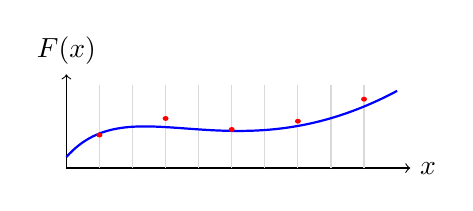
\begin{tikzpicture}[x=0.42cm,y=0.35cm]
 \draw[->] (0,0)--(10.4,0) node[right] {$x$};
 \draw[->] (0,0)--(0,3.4) node[above] {$F(x)$};
 \foreach \x in {1,...,9} {\draw[gray!30] (\x,0)--(\x,3);}
 \draw[blue,thick] (0,0.4) .. controls (2,3.1) and (5,-0.4) .. (10,2.8);
 \foreach \x/\y in {1/1.2,3/1.8,5/1.4,7/1.7,9/2.5}
   \fill[red] (\x,\y) circle (0.09);
\end{tikzpicture}
\end{center}
The next comparison uses Theorem~\ref{thm:74} and Equation~\ref{eq:75}. The construction uses a finite family of examples with different paragraph lengths. Some sentences are short. Others follow the dependence of an estimate on its parameters, introduce a counterexample, and explain why a nearby bound must be reconsidered after an insertion.

\lipsum[3]

\section{A changing estimate: case 077}\label{unit:76}
A local change should remain attached to its source even when surrounding material moves. We compare the displayed argument with the current source version, rather than treating the last compiled page number as a permanent identity.

\lipsum[19-20]
\begin{align}\label{eq:76}
 F_k(x+h)&=F_k(x)+hF_k'(x)+\frac{h^2}{2}F_k''(x)+O(h^3),\\
 \int_0^1 t^k(1-t)\,dt&=\frac{1}{(k+1)(k+2)}.
\end{align}
\begin{theorem}\label{thm:76}
For the finite family in case 77, the normalized error is bounded by $C_k h^2$ whenever $0<h<1$. The constant may depend on $k$ but is independent of the location of the edited paragraph.
\end{theorem}
\begin{proof}
Expand the two terms, collect their first-order contributions, and apply the
triangle inequality. The remaining integral is bounded on the compact interval,
so the asserted estimate follows. This argument also applies after a line break
moves the statement to the next page.
\end{proof}
The next comparison uses Theorem~\ref{thm:75} and Equation~\ref{eq:76}. An observer can return to an earlier part of the document while compilation continues. The relevant statement, equation and hyperlink must still belong to the page actually displayed, including when line wrapping pushes a later theorem across a page boundary.

\lipsum[8]

\section{A changing estimate: case 078}\label{unit:77}
The construction uses a finite family of examples with different paragraph lengths. Some sentences are short. Others follow the dependence of an estimate on its parameters, introduce a counterexample, and explain why a nearby bound must be reconsidered after an insertion.

\lipsum[22-23]
\begin{align}\label{eq:77}
 F_k(x+h)&=F_k(x)+hF_k'(x)+\frac{h^2}{2}F_k''(x)+O(h^3),\\
 \int_0^1 t^k(1-t)\,dt&=\frac{1}{(k+1)(k+2)}.
\end{align}
\begin{theorem}\label{thm:77}
For the finite family in case 78, the normalized error is bounded by $C_k h^2$ whenever $0<h<1$. The constant may depend on $k$ but is independent of the location of the edited paragraph.
\end{theorem}
\begin{proof}
Expand the two terms, collect their first-order contributions, and apply the
triangle inequality. The remaining integral is bounded on the compact interval,
so the asserted estimate follows. This argument also applies after a line break
moves the statement to the next page.
\end{proof}
The next comparison uses Theorem~\ref{thm:76} and Equation~\ref{eq:77}. The proof separates the algebraic estimate from the geometric example. This makes the document useful for edits to prose, formulas, headings and diagrams, while retaining enough ordinary text to exercise paragraph breaking and natural pagination.

\lipsum[13]

\section{A changing estimate: case 079}\label{unit:78}
An observer can return to an earlier part of the document while compilation continues. The relevant statement, equation and hyperlink must still belong to the page actually displayed, including when line wrapping pushes a later theorem across a page boundary.

\lipsum[25-26]
\begin{align}\label{eq:78}
 F_k(x+h)&=F_k(x)+hF_k'(x)+\frac{h^2}{2}F_k''(x)+O(h^3),\\
 \int_0^1 t^k(1-t)\,dt&=\frac{1}{(k+1)(k+2)}.
\end{align}
\begin{lemma}\label{thm:78}
For the finite family in case 79, the normalized error is bounded by $C_k h^2$ whenever $0<h<1$. The constant may depend on $k$ but is independent of the location of the edited paragraph.
\end{lemma}
\begin{proof}
Expand the two terms, collect their first-order contributions, and apply the
triangle inequality. The remaining integral is bounded on the compact interval,
so the asserted estimate follows. This argument also applies after a line break
moves the statement to the next page.
\end{proof}
The next comparison uses Theorem~\ref{thm:77} and Equation~\ref{eq:78}. A local change should remain attached to its source even when surrounding material moves. We compare the displayed argument with the current source version, rather than treating the last compiled page number as a permanent identity.

\lipsum[18]

\section{A changing estimate: case 080}\label{unit:79}
The proof separates the algebraic estimate from the geometric example. This makes the document useful for edits to prose, formulas, headings and diagrams, while retaining enough ordinary text to exercise paragraph breaking and natural pagination.

\lipsum[28-29]
\begin{align}\label{eq:79}
 F_k(x+h)&=F_k(x)+hF_k'(x)+\frac{h^2}{2}F_k''(x)+O(h^3),\\
 \int_0^1 t^k(1-t)\,dt&=\frac{1}{(k+1)(k+2)}.
\end{align}
\begin{theorem}\label{thm:79}
For the finite family in case 80, the normalized error is bounded by $C_k h^2$ whenever $0<h<1$. The constant may depend on $k$ but is independent of the location of the edited paragraph.
\end{theorem}
\begin{proof}
Expand the two terms, collect their first-order contributions, and apply the
triangle inequality. The remaining integral is bounded on the compact interval,
so the asserted estimate follows. This argument also applies after a line break
moves the statement to the next page.
\end{proof}
The next comparison uses Theorem~\ref{thm:78} and Equation~\ref{eq:79}. The construction uses a finite family of examples with different paragraph lengths. Some sentences are short. Others follow the dependence of an estimate on its parameters, introduce a counterexample, and explain why a nearby bound must be reconsidered after an insertion.

\lipsum[23]

\section{A changing estimate: case 081}\label{unit:80}
A local change should remain attached to its source even when surrounding material moves. We compare the displayed argument with the current source version, rather than treating the last compiled page number as a permanent identity.

\lipsum[1-2]
\begin{align}\label{eq:80}
 F_k(x+h)&=F_k(x)+hF_k'(x)+\frac{h^2}{2}F_k''(x)+O(h^3),\\
 \int_0^1 t^k(1-t)\,dt&=\frac{1}{(k+1)(k+2)}.
\end{align}
\begin{theorem}\label{thm:80}
For the finite family in case 81, the normalized error is bounded by $C_k h^2$ whenever $0<h<1$. The constant may depend on $k$ but is independent of the location of the edited paragraph.
\end{theorem}
\begin{proof}
Expand the two terms, collect their first-order contributions, and apply the
triangle inequality. The remaining integral is bounded on the compact interval,
so the asserted estimate follows. This argument also applies after a line break
moves the statement to the next page.
\end{proof}
The next comparison uses Theorem~\ref{thm:79} and Equation~\ref{eq:80}. An observer can return to an earlier part of the document while compilation continues. The relevant statement, equation and hyperlink must still belong to the page actually displayed, including when line wrapping pushes a later theorem across a page boundary.

\lipsum[3]

\section{A changing estimate: case 082}\label{unit:81}
The construction uses a finite family of examples with different paragraph lengths. Some sentences are short. Others follow the dependence of an estimate on its parameters, introduce a counterexample, and explain why a nearby bound must be reconsidered after an insertion.

\lipsum[4-5]
\begin{align}\label{eq:81}
 F_k(x+h)&=F_k(x)+hF_k'(x)+\frac{h^2}{2}F_k''(x)+O(h^3),\\
 \int_0^1 t^k(1-t)\,dt&=\frac{1}{(k+1)(k+2)}.
\end{align}
\begin{lemma}\label{thm:81}
For the finite family in case 82, the normalized error is bounded by $C_k h^2$ whenever $0<h<1$. The constant may depend on $k$ but is independent of the location of the edited paragraph.
\end{lemma}
\begin{proof}
Expand the two terms, collect their first-order contributions, and apply the
triangle inequality. The remaining integral is bounded on the compact interval,
so the asserted estimate follows. This argument also applies after a line break
moves the statement to the next page.
\end{proof}
\begin{center}
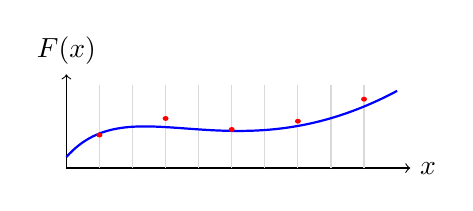
\begin{tikzpicture}[x=0.42cm,y=0.35cm]
 \draw[->] (0,0)--(10.4,0) node[right] {$x$};
 \draw[->] (0,0)--(0,3.4) node[above] {$F(x)$};
 \foreach \x in {1,...,9} {\draw[gray!30] (\x,0)--(\x,3);}
 \draw[blue,thick] (0,0.4) .. controls (2,3.1) and (5,-0.4) .. (10,2.8);
 \foreach \x/\y in {1/1.2,3/1.8,5/1.4,7/1.7,9/2.5}
   \fill[red] (\x,\y) circle (0.09);
\end{tikzpicture}
\end{center}
The next comparison uses Theorem~\ref{thm:80} and Equation~\ref{eq:81}. The proof separates the algebraic estimate from the geometric example. This makes the document useful for edits to prose, formulas, headings and diagrams, while retaining enough ordinary text to exercise paragraph breaking and natural pagination.

\lipsum[8]

\section{A changing estimate: case 083}\label{unit:82}
An observer can return to an earlier part of the document while compilation continues. The relevant statement, equation and hyperlink must still belong to the page actually displayed, including when line wrapping pushes a later theorem across a page boundary.

\lipsum[7-8]
\begin{align}\label{eq:82}
 F_k(x+h)&=F_k(x)+hF_k'(x)+\frac{h^2}{2}F_k''(x)+O(h^3),\\
 \int_0^1 t^k(1-t)\,dt&=\frac{1}{(k+1)(k+2)}.
\end{align}
\begin{theorem}\label{thm:82}
For the finite family in case 83, the normalized error is bounded by $C_k h^2$ whenever $0<h<1$. The constant may depend on $k$ but is independent of the location of the edited paragraph.
\end{theorem}
\begin{proof}
Expand the two terms, collect their first-order contributions, and apply the
triangle inequality. The remaining integral is bounded on the compact interval,
so the asserted estimate follows. This argument also applies after a line break
moves the statement to the next page.
\end{proof}
The next comparison uses Theorem~\ref{thm:81} and Equation~\ref{eq:82}. A local change should remain attached to its source even when surrounding material moves. We compare the displayed argument with the current source version, rather than treating the last compiled page number as a permanent identity.

\lipsum[13]

\section{A changing estimate: case 084}\label{unit:83}
The proof separates the algebraic estimate from the geometric example. This makes the document useful for edits to prose, formulas, headings and diagrams, while retaining enough ordinary text to exercise paragraph breaking and natural pagination.

\lipsum[10-11]
\begin{align}\label{eq:83}
 F_k(x+h)&=F_k(x)+hF_k'(x)+\frac{h^2}{2}F_k''(x)+O(h^3),\\
 \int_0^1 t^k(1-t)\,dt&=\frac{1}{(k+1)(k+2)}.
\end{align}
\begin{theorem}\label{thm:83}
For the finite family in case 84, the normalized error is bounded by $C_k h^2$ whenever $0<h<1$. The constant may depend on $k$ but is independent of the location of the edited paragraph.
\end{theorem}
\begin{proof}
Expand the two terms, collect their first-order contributions, and apply the
triangle inequality. The remaining integral is bounded on the compact interval,
so the asserted estimate follows. This argument also applies after a line break
moves the statement to the next page.
\end{proof}
The next comparison uses Theorem~\ref{thm:82} and Equation~\ref{eq:83}. The construction uses a finite family of examples with different paragraph lengths. Some sentences are short. Others follow the dependence of an estimate on its parameters, introduce a counterexample, and explain why a nearby bound must be reconsidered after an insertion.

\lipsum[18]

\section{A changing estimate: case 085}\label{unit:84}
A local change should remain attached to its source even when surrounding material moves. We compare the displayed argument with the current source version, rather than treating the last compiled page number as a permanent identity.

\lipsum[13-14]
\begin{align}\label{eq:84}
 F_k(x+h)&=F_k(x)+hF_k'(x)+\frac{h^2}{2}F_k''(x)+O(h^3),\\
 \int_0^1 t^k(1-t)\,dt&=\frac{1}{(k+1)(k+2)}.
\end{align}
\begin{lemma}\label{thm:84}
For the finite family in case 85, the normalized error is bounded by $C_k h^2$ whenever $0<h<1$. The constant may depend on $k$ but is independent of the location of the edited paragraph.
\end{lemma}
\begin{proof}
Expand the two terms, collect their first-order contributions, and apply the
triangle inequality. The remaining integral is bounded on the compact interval,
so the asserted estimate follows. This argument also applies after a line break
moves the statement to the next page.
\end{proof}
The next comparison uses Theorem~\ref{thm:83} and Equation~\ref{eq:84}. An observer can return to an earlier part of the document while compilation continues. The relevant statement, equation and hyperlink must still belong to the page actually displayed, including when line wrapping pushes a later theorem across a page boundary.

\lipsum[23]

\section{A changing estimate: case 086}\label{unit:85}
The construction uses a finite family of examples with different paragraph lengths. Some sentences are short. Others follow the dependence of an estimate on its parameters, introduce a counterexample, and explain why a nearby bound must be reconsidered after an insertion.

\lipsum[16-17]
\begin{align}\label{eq:85}
 F_k(x+h)&=F_k(x)+hF_k'(x)+\frac{h^2}{2}F_k''(x)+O(h^3),\\
 \int_0^1 t^k(1-t)\,dt&=\frac{1}{(k+1)(k+2)}.
\end{align}
\begin{theorem}\label{thm:85}
For the finite family in case 86, the normalized error is bounded by $C_k h^2$ whenever $0<h<1$. The constant may depend on $k$ but is independent of the location of the edited paragraph.
\end{theorem}
\begin{proof}
Expand the two terms, collect their first-order contributions, and apply the
triangle inequality. The remaining integral is bounded on the compact interval,
so the asserted estimate follows. This argument also applies after a line break
moves the statement to the next page.
\end{proof}
The next comparison uses Theorem~\ref{thm:84} and Equation~\ref{eq:85}. The proof separates the algebraic estimate from the geometric example. This makes the document useful for edits to prose, formulas, headings and diagrams, while retaining enough ordinary text to exercise paragraph breaking and natural pagination.

\lipsum[3]

\section{A changing estimate: case 087}\label{unit:86}
An observer can return to an earlier part of the document while compilation continues. The relevant statement, equation and hyperlink must still belong to the page actually displayed, including when line wrapping pushes a later theorem across a page boundary.

\lipsum[19-20]
\begin{align}\label{eq:86}
 F_k(x+h)&=F_k(x)+hF_k'(x)+\frac{h^2}{2}F_k''(x)+O(h^3),\\
 \int_0^1 t^k(1-t)\,dt&=\frac{1}{(k+1)(k+2)}.
\end{align}
\begin{theorem}\label{thm:86}
For the finite family in case 87, the normalized error is bounded by $C_k h^2$ whenever $0<h<1$. The constant may depend on $k$ but is independent of the location of the edited paragraph.
\end{theorem}
\begin{proof}
Expand the two terms, collect their first-order contributions, and apply the
triangle inequality. The remaining integral is bounded on the compact interval,
so the asserted estimate follows. This argument also applies after a line break
moves the statement to the next page.
\end{proof}
The next comparison uses Theorem~\ref{thm:85} and Equation~\ref{eq:86}. A local change should remain attached to its source even when surrounding material moves. We compare the displayed argument with the current source version, rather than treating the last compiled page number as a permanent identity.

\lipsum[8]

\section{A changing estimate: case 088}\label{unit:87}
The proof separates the algebraic estimate from the geometric example. This makes the document useful for edits to prose, formulas, headings and diagrams, while retaining enough ordinary text to exercise paragraph breaking and natural pagination.

\lipsum[22-23]
\begin{align}\label{eq:87}
 F_k(x+h)&=F_k(x)+hF_k'(x)+\frac{h^2}{2}F_k''(x)+O(h^3),\\
 \int_0^1 t^k(1-t)\,dt&=\frac{1}{(k+1)(k+2)}.
\end{align}
\begin{lemma}\label{thm:87}
For the finite family in case 88, the normalized error is bounded by $C_k h^2$ whenever $0<h<1$. The constant may depend on $k$ but is independent of the location of the edited paragraph.
\end{lemma}
\begin{proof}
Expand the two terms, collect their first-order contributions, and apply the
triangle inequality. The remaining integral is bounded on the compact interval,
so the asserted estimate follows. This argument also applies after a line break
moves the statement to the next page.
\end{proof}
\begin{center}
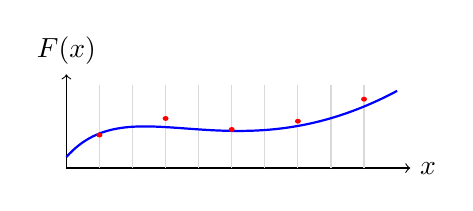
\begin{tikzpicture}[x=0.42cm,y=0.35cm]
 \draw[->] (0,0)--(10.4,0) node[right] {$x$};
 \draw[->] (0,0)--(0,3.4) node[above] {$F(x)$};
 \foreach \x in {1,...,9} {\draw[gray!30] (\x,0)--(\x,3);}
 \draw[blue,thick] (0,0.4) .. controls (2,3.1) and (5,-0.4) .. (10,2.8);
 \foreach \x/\y in {1/1.2,3/1.8,5/1.4,7/1.7,9/2.5}
   \fill[red] (\x,\y) circle (0.09);
\end{tikzpicture}
\end{center}
The next comparison uses Theorem~\ref{thm:86} and Equation~\ref{eq:87}. The construction uses a finite family of examples with different paragraph lengths. Some sentences are short. Others follow the dependence of an estimate on its parameters, introduce a counterexample, and explain why a nearby bound must be reconsidered after an insertion.

\lipsum[13]

\section{A changing estimate: case 089}\label{unit:88}
A local change should remain attached to its source even when surrounding material moves. We compare the displayed argument with the current source version, rather than treating the last compiled page number as a permanent identity.

\lipsum[25-26]
\begin{align}\label{eq:88}
 F_k(x+h)&=F_k(x)+hF_k'(x)+\frac{h^2}{2}F_k''(x)+O(h^3),\\
 \int_0^1 t^k(1-t)\,dt&=\frac{1}{(k+1)(k+2)}.
\end{align}
\begin{theorem}\label{thm:88}
For the finite family in case 89, the normalized error is bounded by $C_k h^2$ whenever $0<h<1$. The constant may depend on $k$ but is independent of the location of the edited paragraph.
\end{theorem}
\begin{proof}
Expand the two terms, collect their first-order contributions, and apply the
triangle inequality. The remaining integral is bounded on the compact interval,
so the asserted estimate follows. This argument also applies after a line break
moves the statement to the next page.
\end{proof}
The next comparison uses Theorem~\ref{thm:87} and Equation~\ref{eq:88}. An observer can return to an earlier part of the document while compilation continues. The relevant statement, equation and hyperlink must still belong to the page actually displayed, including when line wrapping pushes a later theorem across a page boundary.

\lipsum[18]

\section{A changing estimate: case 090}\label{unit:89}
The construction uses a finite family of examples with different paragraph lengths. Some sentences are short. Others follow the dependence of an estimate on its parameters, introduce a counterexample, and explain why a nearby bound must be reconsidered after an insertion.

\lipsum[28-29]
\begin{align}\label{eq:89}
 F_k(x+h)&=F_k(x)+hF_k'(x)+\frac{h^2}{2}F_k''(x)+O(h^3),\\
 \int_0^1 t^k(1-t)\,dt&=\frac{1}{(k+1)(k+2)}.
\end{align}
\begin{theorem}\label{thm:89}
For the finite family in case 90, the normalized error is bounded by $C_k h^2$ whenever $0<h<1$. The constant may depend on $k$ but is independent of the location of the edited paragraph.
\end{theorem}
\begin{proof}
Expand the two terms, collect their first-order contributions, and apply the
triangle inequality. The remaining integral is bounded on the compact interval,
so the asserted estimate follows. This argument also applies after a line break
moves the statement to the next page.
\end{proof}
The next comparison uses Theorem~\ref{thm:88} and Equation~\ref{eq:89}. The proof separates the algebraic estimate from the geometric example. This makes the document useful for edits to prose, formulas, headings and diagrams, while retaining enough ordinary text to exercise paragraph breaking and natural pagination.

\lipsum[23]

\section{A changing estimate: case 091}\label{unit:90}
An observer can return to an earlier part of the document while compilation continues. The relevant statement, equation and hyperlink must still belong to the page actually displayed, including when line wrapping pushes a later theorem across a page boundary.

\lipsum[1-2]
\begin{align}\label{eq:90}
 F_k(x+h)&=F_k(x)+hF_k'(x)+\frac{h^2}{2}F_k''(x)+O(h^3),\\
 \int_0^1 t^k(1-t)\,dt&=\frac{1}{(k+1)(k+2)}.
\end{align}
\begin{lemma}\label{thm:90}
For the finite family in case 91, the normalized error is bounded by $C_k h^2$ whenever $0<h<1$. The constant may depend on $k$ but is independent of the location of the edited paragraph.
\end{lemma}
\begin{proof}
Expand the two terms, collect their first-order contributions, and apply the
triangle inequality. The remaining integral is bounded on the compact interval,
so the asserted estimate follows. This argument also applies after a line break
moves the statement to the next page.
\end{proof}
The next comparison uses Theorem~\ref{thm:89} and Equation~\ref{eq:90}. A local change should remain attached to its source even when surrounding material moves. We compare the displayed argument with the current source version, rather than treating the last compiled page number as a permanent identity.

\lipsum[3]

\section{A changing estimate: case 092}\label{unit:91}
The proof separates the algebraic estimate from the geometric example. This makes the document useful for edits to prose, formulas, headings and diagrams, while retaining enough ordinary text to exercise paragraph breaking and natural pagination.

\lipsum[4-5]
\begin{align}\label{eq:91}
 F_k(x+h)&=F_k(x)+hF_k'(x)+\frac{h^2}{2}F_k''(x)+O(h^3),\\
 \int_0^1 t^k(1-t)\,dt&=\frac{1}{(k+1)(k+2)}.
\end{align}
\begin{theorem}\label{thm:91}
For the finite family in case 92, the normalized error is bounded by $C_k h^2$ whenever $0<h<1$. The constant may depend on $k$ but is independent of the location of the edited paragraph.
\end{theorem}
\begin{proof}
Expand the two terms, collect their first-order contributions, and apply the
triangle inequality. The remaining integral is bounded on the compact interval,
so the asserted estimate follows. This argument also applies after a line break
moves the statement to the next page.
\end{proof}
The next comparison uses Theorem~\ref{thm:90} and Equation~\ref{eq:91}. The construction uses a finite family of examples with different paragraph lengths. Some sentences are short. Others follow the dependence of an estimate on its parameters, introduce a counterexample, and explain why a nearby bound must be reconsidered after an insertion.

\lipsum[8]

\section{A changing estimate: case 093}\label{unit:92}
A local change should remain attached to its source even when surrounding material moves. We compare the displayed argument with the current source version, rather than treating the last compiled page number as a permanent identity.

\lipsum[7-8]
\begin{align}\label{eq:92}
 F_k(x+h)&=F_k(x)+hF_k'(x)+\frac{h^2}{2}F_k''(x)+O(h^3),\\
 \int_0^1 t^k(1-t)\,dt&=\frac{1}{(k+1)(k+2)}.
\end{align}
\begin{theorem}\label{thm:92}
For the finite family in case 93, the normalized error is bounded by $C_k h^2$ whenever $0<h<1$. The constant may depend on $k$ but is independent of the location of the edited paragraph.
\end{theorem}
\begin{proof}
Expand the two terms, collect their first-order contributions, and apply the
triangle inequality. The remaining integral is bounded on the compact interval,
so the asserted estimate follows. This argument also applies after a line break
moves the statement to the next page.
\end{proof}
The next comparison uses Theorem~\ref{thm:91} and Equation~\ref{eq:92}. An observer can return to an earlier part of the document while compilation continues. The relevant statement, equation and hyperlink must still belong to the page actually displayed, including when line wrapping pushes a later theorem across a page boundary.

\lipsum[13]

\section{A changing estimate: case 094}\label{unit:93}
The construction uses a finite family of examples with different paragraph lengths. Some sentences are short. Others follow the dependence of an estimate on its parameters, introduce a counterexample, and explain why a nearby bound must be reconsidered after an insertion.

\lipsum[10-11]
\begin{align}\label{eq:93}
 F_k(x+h)&=F_k(x)+hF_k'(x)+\frac{h^2}{2}F_k''(x)+O(h^3),\\
 \int_0^1 t^k(1-t)\,dt&=\frac{1}{(k+1)(k+2)}.
\end{align}
\begin{lemma}\label{thm:93}
For the finite family in case 94, the normalized error is bounded by $C_k h^2$ whenever $0<h<1$. The constant may depend on $k$ but is independent of the location of the edited paragraph.
\end{lemma}
\begin{proof}
Expand the two terms, collect their first-order contributions, and apply the
triangle inequality. The remaining integral is bounded on the compact interval,
so the asserted estimate follows. This argument also applies after a line break
moves the statement to the next page.
\end{proof}
\begin{center}
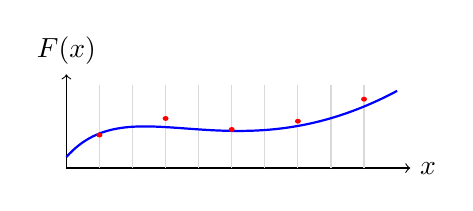
\begin{tikzpicture}[x=0.42cm,y=0.35cm]
 \draw[->] (0,0)--(10.4,0) node[right] {$x$};
 \draw[->] (0,0)--(0,3.4) node[above] {$F(x)$};
 \foreach \x in {1,...,9} {\draw[gray!30] (\x,0)--(\x,3);}
 \draw[blue,thick] (0,0.4) .. controls (2,3.1) and (5,-0.4) .. (10,2.8);
 \foreach \x/\y in {1/1.2,3/1.8,5/1.4,7/1.7,9/2.5}
   \fill[red] (\x,\y) circle (0.09);
\end{tikzpicture}
\end{center}
The next comparison uses Theorem~\ref{thm:92} and Equation~\ref{eq:93}. The proof separates the algebraic estimate from the geometric example. This makes the document useful for edits to prose, formulas, headings and diagrams, while retaining enough ordinary text to exercise paragraph breaking and natural pagination.

\lipsum[18]

\section{A changing estimate: case 095}\label{unit:94}
An observer can return to an earlier part of the document while compilation continues. The relevant statement, equation and hyperlink must still belong to the page actually displayed, including when line wrapping pushes a later theorem across a page boundary.

\lipsum[13-14]
\begin{align}\label{eq:94}
 F_k(x+h)&=F_k(x)+hF_k'(x)+\frac{h^2}{2}F_k''(x)+O(h^3),\\
 \int_0^1 t^k(1-t)\,dt&=\frac{1}{(k+1)(k+2)}.
\end{align}
\begin{theorem}\label{thm:94}
For the finite family in case 95, the normalized error is bounded by $C_k h^2$ whenever $0<h<1$. The constant may depend on $k$ but is independent of the location of the edited paragraph.
\end{theorem}
\begin{proof}
Expand the two terms, collect their first-order contributions, and apply the
triangle inequality. The remaining integral is bounded on the compact interval,
so the asserted estimate follows. This argument also applies after a line break
moves the statement to the next page.
\end{proof}
The next comparison uses Theorem~\ref{thm:93} and Equation~\ref{eq:94}. A local change should remain attached to its source even when surrounding material moves. We compare the displayed argument with the current source version, rather than treating the last compiled page number as a permanent identity.

\lipsum[23]

\section{A changing estimate: case 096}\label{unit:95}
The proof separates the algebraic estimate from the geometric example. This makes the document useful for edits to prose, formulas, headings and diagrams, while retaining enough ordinary text to exercise paragraph breaking and natural pagination.

\lipsum[16-17]
\begin{align}\label{eq:95}
 F_k(x+h)&=F_k(x)+hF_k'(x)+\frac{h^2}{2}F_k''(x)+O(h^3),\\
 \int_0^1 t^k(1-t)\,dt&=\frac{1}{(k+1)(k+2)}.
\end{align}
\begin{theorem}\label{thm:95}
For the finite family in case 96, the normalized error is bounded by $C_k h^2$ whenever $0<h<1$. The constant may depend on $k$ but is independent of the location of the edited paragraph.
\end{theorem}
\begin{proof}
Expand the two terms, collect their first-order contributions, and apply the
triangle inequality. The remaining integral is bounded on the compact interval,
so the asserted estimate follows. This argument also applies after a line break
moves the statement to the next page.
\end{proof}
The next comparison uses Theorem~\ref{thm:94} and Equation~\ref{eq:95}. The construction uses a finite family of examples with different paragraph lengths. Some sentences are short. Others follow the dependence of an estimate on its parameters, introduce a counterexample, and explain why a nearby bound must be reconsidered after an insertion.

\lipsum[3]

\section{A changing estimate: case 097}\label{unit:96}
A local change should remain attached to its source even when surrounding material moves. We compare the displayed argument with the current source version, rather than treating the last compiled page number as a permanent identity.

\lipsum[19-20]
\begin{align}\label{eq:96}
 F_k(x+h)&=F_k(x)+hF_k'(x)+\frac{h^2}{2}F_k''(x)+O(h^3),\\
 \int_0^1 t^k(1-t)\,dt&=\frac{1}{(k+1)(k+2)}.
\end{align}
\begin{lemma}\label{thm:96}
For the finite family in case 97, the normalized error is bounded by $C_k h^2$ whenever $0<h<1$. The constant may depend on $k$ but is independent of the location of the edited paragraph.
\end{lemma}
\begin{proof}
Expand the two terms, collect their first-order contributions, and apply the
triangle inequality. The remaining integral is bounded on the compact interval,
so the asserted estimate follows. This argument also applies after a line break
moves the statement to the next page.
\end{proof}
The next comparison uses Theorem~\ref{thm:95} and Equation~\ref{eq:96}. An observer can return to an earlier part of the document while compilation continues. The relevant statement, equation and hyperlink must still belong to the page actually displayed, including when line wrapping pushes a later theorem across a page boundary.

\lipsum[8]

\section{A changing estimate: case 098}\label{unit:97}
The construction uses a finite family of examples with different paragraph lengths. Some sentences are short. Others follow the dependence of an estimate on its parameters, introduce a counterexample, and explain why a nearby bound must be reconsidered after an insertion.

\lipsum[22-23]
\begin{align}\label{eq:97}
 F_k(x+h)&=F_k(x)+hF_k'(x)+\frac{h^2}{2}F_k''(x)+O(h^3),\\
 \int_0^1 t^k(1-t)\,dt&=\frac{1}{(k+1)(k+2)}.
\end{align}
\begin{theorem}\label{thm:97}
For the finite family in case 98, the normalized error is bounded by $C_k h^2$ whenever $0<h<1$. The constant may depend on $k$ but is independent of the location of the edited paragraph.
\end{theorem}
\begin{proof}
Expand the two terms, collect their first-order contributions, and apply the
triangle inequality. The remaining integral is bounded on the compact interval,
so the asserted estimate follows. This argument also applies after a line break
moves the statement to the next page.
\end{proof}
The next comparison uses Theorem~\ref{thm:96} and Equation~\ref{eq:97}. The proof separates the algebraic estimate from the geometric example. This makes the document useful for edits to prose, formulas, headings and diagrams, while retaining enough ordinary text to exercise paragraph breaking and natural pagination.

\lipsum[13]

\section{A changing estimate: case 099}\label{unit:98}
An observer can return to an earlier part of the document while compilation continues. The relevant statement, equation and hyperlink must still belong to the page actually displayed, including when line wrapping pushes a later theorem across a page boundary.

\lipsum[25-26]
\begin{align}\label{eq:98}
 F_k(x+h)&=F_k(x)+hF_k'(x)+\frac{h^2}{2}F_k''(x)+O(h^3),\\
 \int_0^1 t^k(1-t)\,dt&=\frac{1}{(k+1)(k+2)}.
\end{align}
\begin{theorem}\label{thm:98}
For the finite family in case 99, the normalized error is bounded by $C_k h^2$ whenever $0<h<1$. The constant may depend on $k$ but is independent of the location of the edited paragraph.
\end{theorem}
\begin{proof}
Expand the two terms, collect their first-order contributions, and apply the
triangle inequality. The remaining integral is bounded on the compact interval,
so the asserted estimate follows. This argument also applies after a line break
moves the statement to the next page.
\end{proof}
The next comparison uses Theorem~\ref{thm:97} and Equation~\ref{eq:98}. A local change should remain attached to its source even when surrounding material moves. We compare the displayed argument with the current source version, rather than treating the last compiled page number as a permanent identity.

\lipsum[18]

\section{A changing estimate: case 100}\label{unit:99}
The proof separates the algebraic estimate from the geometric example. This makes the document useful for edits to prose, formulas, headings and diagrams, while retaining enough ordinary text to exercise paragraph breaking and natural pagination.

\lipsum[28-29]
\begin{align}\label{eq:99}
 F_k(x+h)&=F_k(x)+hF_k'(x)+\frac{h^2}{2}F_k''(x)+O(h^3),\\
 \int_0^1 t^k(1-t)\,dt&=\frac{1}{(k+1)(k+2)}.
\end{align}
\begin{lemma}\label{thm:99}
For the finite family in case 100, the normalized error is bounded by $C_k h^2$ whenever $0<h<1$. The constant may depend on $k$ but is independent of the location of the edited paragraph.
\end{lemma}
\begin{proof}
Expand the two terms, collect their first-order contributions, and apply the
triangle inequality. The remaining integral is bounded on the compact interval,
so the asserted estimate follows. This argument also applies after a line break
moves the statement to the next page.
\end{proof}
\begin{center}
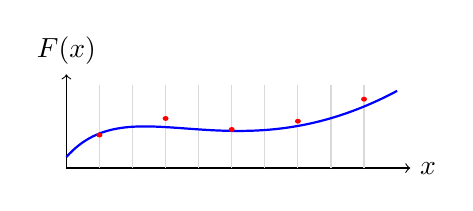
\begin{tikzpicture}[x=0.42cm,y=0.35cm]
 \draw[->] (0,0)--(10.4,0) node[right] {$x$};
 \draw[->] (0,0)--(0,3.4) node[above] {$F(x)$};
 \foreach \x in {1,...,9} {\draw[gray!30] (\x,0)--(\x,3);}
 \draw[blue,thick] (0,0.4) .. controls (2,3.1) and (5,-0.4) .. (10,2.8);
 \foreach \x/\y in {1/1.2,3/1.8,5/1.4,7/1.7,9/2.5}
   \fill[red] (\x,\y) circle (0.09);
\end{tikzpicture}
\end{center}
The next comparison uses Theorem~\ref{thm:98} and Equation~\ref{eq:99}. The construction uses a finite family of examples with different paragraph lengths. Some sentences are short. Others follow the dependence of an estimate on its parameters, introduce a counterexample, and explain why a nearby bound must be reconsidered after an insertion.

\lipsum[23]

\section{A changing estimate: case 101}\label{unit:100}
A local change should remain attached to its source even when surrounding material moves. We compare the displayed argument with the current source version, rather than treating the last compiled page number as a permanent identity.

\lipsum[1-2]
\begin{align}\label{eq:100}
 F_k(x+h)&=F_k(x)+hF_k'(x)+\frac{h^2}{2}F_k''(x)+O(h^3),\\
 \int_0^1 t^k(1-t)\,dt&=\frac{1}{(k+1)(k+2)}.
\end{align}
\begin{theorem}\label{thm:100}
For the finite family in case 101, the normalized error is bounded by $C_k h^2$ whenever $0<h<1$. The constant may depend on $k$ but is independent of the location of the edited paragraph.
\end{theorem}
\begin{proof}
Expand the two terms, collect their first-order contributions, and apply the
triangle inequality. The remaining integral is bounded on the compact interval,
so the asserted estimate follows. This argument also applies after a line break
moves the statement to the next page.
\end{proof}
The next comparison uses Theorem~\ref{thm:99} and Equation~\ref{eq:100}. An observer can return to an earlier part of the document while compilation continues. The relevant statement, equation and hyperlink must still belong to the page actually displayed, including when line wrapping pushes a later theorem across a page boundary.

\lipsum[3]

\section{A changing estimate: case 102}\label{unit:101}
The construction uses a finite family of examples with different paragraph lengths. Some sentences are short. Others follow the dependence of an estimate on its parameters, introduce a counterexample, and explain why a nearby bound must be reconsidered after an insertion.

\lipsum[4-5]
\begin{align}\label{eq:101}
 F_k(x+h)&=F_k(x)+hF_k'(x)+\frac{h^2}{2}F_k''(x)+O(h^3),\\
 \int_0^1 t^k(1-t)\,dt&=\frac{1}{(k+1)(k+2)}.
\end{align}
\begin{theorem}\label{thm:101}
For the finite family in case 102, the normalized error is bounded by $C_k h^2$ whenever $0<h<1$. The constant may depend on $k$ but is independent of the location of the edited paragraph.
\end{theorem}
\begin{proof}
Expand the two terms, collect their first-order contributions, and apply the
triangle inequality. The remaining integral is bounded on the compact interval,
so the asserted estimate follows. This argument also applies after a line break
moves the statement to the next page.
\end{proof}
The next comparison uses Theorem~\ref{thm:100} and Equation~\ref{eq:101}. The proof separates the algebraic estimate from the geometric example. This makes the document useful for edits to prose, formulas, headings and diagrams, while retaining enough ordinary text to exercise paragraph breaking and natural pagination.

\lipsum[8]

\section{A changing estimate: case 103}\label{unit:102}
An observer can return to an earlier part of the document while compilation continues. The relevant statement, equation and hyperlink must still belong to the page actually displayed, including when line wrapping pushes a later theorem across a page boundary.

\lipsum[7-8]
\begin{align}\label{eq:102}
 F_k(x+h)&=F_k(x)+hF_k'(x)+\frac{h^2}{2}F_k''(x)+O(h^3),\\
 \int_0^1 t^k(1-t)\,dt&=\frac{1}{(k+1)(k+2)}.
\end{align}
\begin{lemma}\label{thm:102}
For the finite family in case 103, the normalized error is bounded by $C_k h^2$ whenever $0<h<1$. The constant may depend on $k$ but is independent of the location of the edited paragraph.
\end{lemma}
\begin{proof}
Expand the two terms, collect their first-order contributions, and apply the
triangle inequality. The remaining integral is bounded on the compact interval,
so the asserted estimate follows. This argument also applies after a line break
moves the statement to the next page.
\end{proof}
The next comparison uses Theorem~\ref{thm:101} and Equation~\ref{eq:102}. A local change should remain attached to its source even when surrounding material moves. We compare the displayed argument with the current source version, rather than treating the last compiled page number as a permanent identity.

\lipsum[13]

\section{A changing estimate: case 104}\label{unit:103}
The proof separates the algebraic estimate from the geometric example. This makes the document useful for edits to prose, formulas, headings and diagrams, while retaining enough ordinary text to exercise paragraph breaking and natural pagination.

\lipsum[10-11]
\begin{align}\label{eq:103}
 F_k(x+h)&=F_k(x)+hF_k'(x)+\frac{h^2}{2}F_k''(x)+O(h^3),\\
 \int_0^1 t^k(1-t)\,dt&=\frac{1}{(k+1)(k+2)}.
\end{align}
\begin{theorem}\label{thm:103}
For the finite family in case 104, the normalized error is bounded by $C_k h^2$ whenever $0<h<1$. The constant may depend on $k$ but is independent of the location of the edited paragraph.
\end{theorem}
\begin{proof}
Expand the two terms, collect their first-order contributions, and apply the
triangle inequality. The remaining integral is bounded on the compact interval,
so the asserted estimate follows. This argument also applies after a line break
moves the statement to the next page.
\end{proof}
The next comparison uses Theorem~\ref{thm:102} and Equation~\ref{eq:103}. The construction uses a finite family of examples with different paragraph lengths. Some sentences are short. Others follow the dependence of an estimate on its parameters, introduce a counterexample, and explain why a nearby bound must be reconsidered after an insertion.

\lipsum[18]

\section{A changing estimate: case 105}\label{unit:104}
A local change should remain attached to its source even when surrounding material moves. We compare the displayed argument with the current source version, rather than treating the last compiled page number as a permanent identity.

\lipsum[13-14]
\begin{align}\label{eq:104}
 F_k(x+h)&=F_k(x)+hF_k'(x)+\frac{h^2}{2}F_k''(x)+O(h^3),\\
 \int_0^1 t^k(1-t)\,dt&=\frac{1}{(k+1)(k+2)}.
\end{align}
\begin{theorem}\label{thm:104}
For the finite family in case 105, the normalized error is bounded by $C_k h^2$ whenever $0<h<1$. The constant may depend on $k$ but is independent of the location of the edited paragraph.
\end{theorem}
\begin{proof}
Expand the two terms, collect their first-order contributions, and apply the
triangle inequality. The remaining integral is bounded on the compact interval,
so the asserted estimate follows. This argument also applies after a line break
moves the statement to the next page.
\end{proof}
The next comparison uses Theorem~\ref{thm:103} and Equation~\ref{eq:104}. An observer can return to an earlier part of the document while compilation continues. The relevant statement, equation and hyperlink must still belong to the page actually displayed, including when line wrapping pushes a later theorem across a page boundary.

\lipsum[23]

\section{A changing estimate: case 106}\label{unit:105}
The construction uses a finite family of examples with different paragraph lengths. Some sentences are short. Others follow the dependence of an estimate on its parameters, introduce a counterexample, and explain why a nearby bound must be reconsidered after an insertion.

\lipsum[16-17]
\begin{align}\label{eq:105}
 F_k(x+h)&=F_k(x)+hF_k'(x)+\frac{h^2}{2}F_k''(x)+O(h^3),\\
 \int_0^1 t^k(1-t)\,dt&=\frac{1}{(k+1)(k+2)}.
\end{align}
\begin{lemma}\label{thm:105}
For the finite family in case 106, the normalized error is bounded by $C_k h^2$ whenever $0<h<1$. The constant may depend on $k$ but is independent of the location of the edited paragraph.
\end{lemma}
\begin{proof}
Expand the two terms, collect their first-order contributions, and apply the
triangle inequality. The remaining integral is bounded on the compact interval,
so the asserted estimate follows. This argument also applies after a line break
moves the statement to the next page.
\end{proof}
\begin{center}
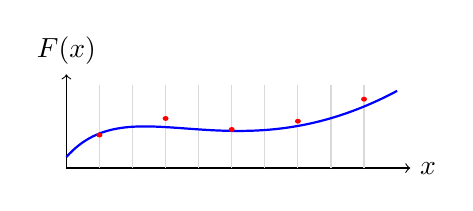
\begin{tikzpicture}[x=0.42cm,y=0.35cm]
 \draw[->] (0,0)--(10.4,0) node[right] {$x$};
 \draw[->] (0,0)--(0,3.4) node[above] {$F(x)$};
 \foreach \x in {1,...,9} {\draw[gray!30] (\x,0)--(\x,3);}
 \draw[blue,thick] (0,0.4) .. controls (2,3.1) and (5,-0.4) .. (10,2.8);
 \foreach \x/\y in {1/1.2,3/1.8,5/1.4,7/1.7,9/2.5}
   \fill[red] (\x,\y) circle (0.09);
\end{tikzpicture}
\end{center}
The next comparison uses Theorem~\ref{thm:104} and Equation~\ref{eq:105}. The proof separates the algebraic estimate from the geometric example. This makes the document useful for edits to prose, formulas, headings and diagrams, while retaining enough ordinary text to exercise paragraph breaking and natural pagination.

\lipsum[3]

\section{A changing estimate: case 107}\label{unit:106}
An observer can return to an earlier part of the document while compilation continues. The relevant statement, equation and hyperlink must still belong to the page actually displayed, including when line wrapping pushes a later theorem across a page boundary.

\lipsum[19-20]
\begin{align}\label{eq:106}
 F_k(x+h)&=F_k(x)+hF_k'(x)+\frac{h^2}{2}F_k''(x)+O(h^3),\\
 \int_0^1 t^k(1-t)\,dt&=\frac{1}{(k+1)(k+2)}.
\end{align}
\begin{theorem}\label{thm:106}
For the finite family in case 107, the normalized error is bounded by $C_k h^2$ whenever $0<h<1$. The constant may depend on $k$ but is independent of the location of the edited paragraph.
\end{theorem}
\begin{proof}
Expand the two terms, collect their first-order contributions, and apply the
triangle inequality. The remaining integral is bounded on the compact interval,
so the asserted estimate follows. This argument also applies after a line break
moves the statement to the next page.
\end{proof}
The next comparison uses Theorem~\ref{thm:105} and Equation~\ref{eq:106}. A local change should remain attached to its source even when surrounding material moves. We compare the displayed argument with the current source version, rather than treating the last compiled page number as a permanent identity.

\lipsum[8]

\section{A changing estimate: case 108}\label{unit:107}
The proof separates the algebraic estimate from the geometric example. This makes the document useful for edits to prose, formulas, headings and diagrams, while retaining enough ordinary text to exercise paragraph breaking and natural pagination.

\lipsum[22-23]
\begin{align}\label{eq:107}
 F_k(x+h)&=F_k(x)+hF_k'(x)+\frac{h^2}{2}F_k''(x)+O(h^3),\\
 \int_0^1 t^k(1-t)\,dt&=\frac{1}{(k+1)(k+2)}.
\end{align}
\begin{theorem}\label{thm:107}
For the finite family in case 108, the normalized error is bounded by $C_k h^2$ whenever $0<h<1$. The constant may depend on $k$ but is independent of the location of the edited paragraph.
\end{theorem}
\begin{proof}
Expand the two terms, collect their first-order contributions, and apply the
triangle inequality. The remaining integral is bounded on the compact interval,
so the asserted estimate follows. This argument also applies after a line break
moves the statement to the next page.
\end{proof}
The next comparison uses Theorem~\ref{thm:106} and Equation~\ref{eq:107}. The construction uses a finite family of examples with different paragraph lengths. Some sentences are short. Others follow the dependence of an estimate on its parameters, introduce a counterexample, and explain why a nearby bound must be reconsidered after an insertion.

\lipsum[13]

\section{A changing estimate: case 109}\label{unit:108}
A local change should remain attached to its source even when surrounding material moves. We compare the displayed argument with the current source version, rather than treating the last compiled page number as a permanent identity.

\lipsum[25-26]
\begin{align}\label{eq:108}
 F_k(x+h)&=F_k(x)+hF_k'(x)+\frac{h^2}{2}F_k''(x)+O(h^3),\\
 \int_0^1 t^k(1-t)\,dt&=\frac{1}{(k+1)(k+2)}.
\end{align}
\begin{lemma}\label{thm:108}
For the finite family in case 109, the normalized error is bounded by $C_k h^2$ whenever $0<h<1$. The constant may depend on $k$ but is independent of the location of the edited paragraph.
\end{lemma}
\begin{proof}
Expand the two terms, collect their first-order contributions, and apply the
triangle inequality. The remaining integral is bounded on the compact interval,
so the asserted estimate follows. This argument also applies after a line break
moves the statement to the next page.
\end{proof}
The next comparison uses Theorem~\ref{thm:107} and Equation~\ref{eq:108}. An observer can return to an earlier part of the document while compilation continues. The relevant statement, equation and hyperlink must still belong to the page actually displayed, including when line wrapping pushes a later theorem across a page boundary.

\lipsum[18]

\section{A changing estimate: case 110}\label{unit:109}
The construction uses a finite family of examples with different paragraph lengths. Some sentences are short. Others follow the dependence of an estimate on its parameters, introduce a counterexample, and explain why a nearby bound must be reconsidered after an insertion.

\lipsum[28-29]
\begin{align}\label{eq:109}
 F_k(x+h)&=F_k(x)+hF_k'(x)+\frac{h^2}{2}F_k''(x)+O(h^3),\\
 \int_0^1 t^k(1-t)\,dt&=\frac{1}{(k+1)(k+2)}.
\end{align}
\begin{theorem}\label{thm:109}
For the finite family in case 110, the normalized error is bounded by $C_k h^2$ whenever $0<h<1$. The constant may depend on $k$ but is independent of the location of the edited paragraph.
\end{theorem}
\begin{proof}
Expand the two terms, collect their first-order contributions, and apply the
triangle inequality. The remaining integral is bounded on the compact interval,
so the asserted estimate follows. This argument also applies after a line break
moves the statement to the next page.
\end{proof}
The next comparison uses Theorem~\ref{thm:108} and Equation~\ref{eq:109}. The proof separates the algebraic estimate from the geometric example. This makes the document useful for edits to prose, formulas, headings and diagrams, while retaining enough ordinary text to exercise paragraph breaking and natural pagination.

\lipsum[23]

\section{A changing estimate: case 111}\label{unit:110}
An observer can return to an earlier part of the document while compilation continues. The relevant statement, equation and hyperlink must still belong to the page actually displayed, including when line wrapping pushes a later theorem across a page boundary.

\lipsum[1-2]
\begin{align}\label{eq:110}
 F_k(x+h)&=F_k(x)+hF_k'(x)+\frac{h^2}{2}F_k''(x)+O(h^3),\\
 \int_0^1 t^k(1-t)\,dt&=\frac{1}{(k+1)(k+2)}.
\end{align}
\begin{theorem}\label{thm:110}
For the finite family in case 111, the normalized error is bounded by $C_k h^2$ whenever $0<h<1$. The constant may depend on $k$ but is independent of the location of the edited paragraph.
\end{theorem}
\begin{proof}
Expand the two terms, collect their first-order contributions, and apply the
triangle inequality. The remaining integral is bounded on the compact interval,
so the asserted estimate follows. This argument also applies after a line break
moves the statement to the next page.
\end{proof}
The next comparison uses Theorem~\ref{thm:109} and Equation~\ref{eq:110}. A local change should remain attached to its source even when surrounding material moves. We compare the displayed argument with the current source version, rather than treating the last compiled page number as a permanent identity.

\lipsum[3]

\section{A changing estimate: case 112}\label{unit:111}
The proof separates the algebraic estimate from the geometric example. This makes the document useful for edits to prose, formulas, headings and diagrams, while retaining enough ordinary text to exercise paragraph breaking and natural pagination.

\lipsum[4-5]
\begin{align}\label{eq:111}
 F_k(x+h)&=F_k(x)+hF_k'(x)+\frac{h^2}{2}F_k''(x)+O(h^3),\\
 \int_0^1 t^k(1-t)\,dt&=\frac{1}{(k+1)(k+2)}.
\end{align}
\begin{lemma}\label{thm:111}
For the finite family in case 112, the normalized error is bounded by $C_k h^2$ whenever $0<h<1$. The constant may depend on $k$ but is independent of the location of the edited paragraph.
\end{lemma}
\begin{proof}
Expand the two terms, collect their first-order contributions, and apply the
triangle inequality. The remaining integral is bounded on the compact interval,
so the asserted estimate follows. This argument also applies after a line break
moves the statement to the next page.
\end{proof}
\begin{center}
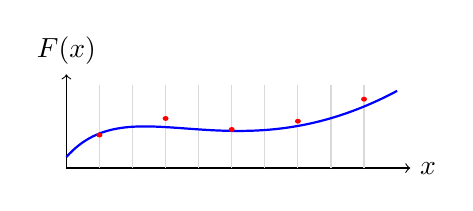
\begin{tikzpicture}[x=0.42cm,y=0.35cm]
 \draw[->] (0,0)--(10.4,0) node[right] {$x$};
 \draw[->] (0,0)--(0,3.4) node[above] {$F(x)$};
 \foreach \x in {1,...,9} {\draw[gray!30] (\x,0)--(\x,3);}
 \draw[blue,thick] (0,0.4) .. controls (2,3.1) and (5,-0.4) .. (10,2.8);
 \foreach \x/\y in {1/1.2,3/1.8,5/1.4,7/1.7,9/2.5}
   \fill[red] (\x,\y) circle (0.09);
\end{tikzpicture}
\end{center}
The next comparison uses Theorem~\ref{thm:110} and Equation~\ref{eq:111}. The construction uses a finite family of examples with different paragraph lengths. Some sentences are short. Others follow the dependence of an estimate on its parameters, introduce a counterexample, and explain why a nearby bound must be reconsidered after an insertion.

\lipsum[8]

\section{A changing estimate: case 113}\label{unit:112}
A local change should remain attached to its source even when surrounding material moves. We compare the displayed argument with the current source version, rather than treating the last compiled page number as a permanent identity.

\lipsum[7-8]
\begin{align}\label{eq:112}
 F_k(x+h)&=F_k(x)+hF_k'(x)+\frac{h^2}{2}F_k''(x)+O(h^3),\\
 \int_0^1 t^k(1-t)\,dt&=\frac{1}{(k+1)(k+2)}.
\end{align}
\begin{theorem}\label{thm:112}
For the finite family in case 113, the normalized error is bounded by $C_k h^2$ whenever $0<h<1$. The constant may depend on $k$ but is independent of the location of the edited paragraph.
\end{theorem}
\begin{proof}
Expand the two terms, collect their first-order contributions, and apply the
triangle inequality. The remaining integral is bounded on the compact interval,
so the asserted estimate follows. This argument also applies after a line break
moves the statement to the next page.
\end{proof}
The next comparison uses Theorem~\ref{thm:111} and Equation~\ref{eq:112}. An observer can return to an earlier part of the document while compilation continues. The relevant statement, equation and hyperlink must still belong to the page actually displayed, including when line wrapping pushes a later theorem across a page boundary.

\lipsum[13]

\section{A changing estimate: case 114}\label{unit:113}
The construction uses a finite family of examples with different paragraph lengths. Some sentences are short. Others follow the dependence of an estimate on its parameters, introduce a counterexample, and explain why a nearby bound must be reconsidered after an insertion.

\lipsum[10-11]
\begin{align}\label{eq:113}
 F_k(x+h)&=F_k(x)+hF_k'(x)+\frac{h^2}{2}F_k''(x)+O(h^3),\\
 \int_0^1 t^k(1-t)\,dt&=\frac{1}{(k+1)(k+2)}.
\end{align}
\begin{theorem}\label{thm:113}
For the finite family in case 114, the normalized error is bounded by $C_k h^2$ whenever $0<h<1$. The constant may depend on $k$ but is independent of the location of the edited paragraph.
\end{theorem}
\begin{proof}
Expand the two terms, collect their first-order contributions, and apply the
triangle inequality. The remaining integral is bounded on the compact interval,
so the asserted estimate follows. This argument also applies after a line break
moves the statement to the next page.
\end{proof}
The next comparison uses Theorem~\ref{thm:112} and Equation~\ref{eq:113}. The proof separates the algebraic estimate from the geometric example. This makes the document useful for edits to prose, formulas, headings and diagrams, while retaining enough ordinary text to exercise paragraph breaking and natural pagination.

\lipsum[18]

\section{A changing estimate: case 115}\label{unit:114}
An observer can return to an earlier part of the document while compilation continues. The relevant statement, equation and hyperlink must still belong to the page actually displayed, including when line wrapping pushes a later theorem across a page boundary.

\lipsum[13-14]
\begin{align}\label{eq:114}
 F_k(x+h)&=F_k(x)+hF_k'(x)+\frac{h^2}{2}F_k''(x)+O(h^3),\\
 \int_0^1 t^k(1-t)\,dt&=\frac{1}{(k+1)(k+2)}.
\end{align}
\begin{lemma}\label{thm:114}
For the finite family in case 115, the normalized error is bounded by $C_k h^2$ whenever $0<h<1$. The constant may depend on $k$ but is independent of the location of the edited paragraph.
\end{lemma}
\begin{proof}
Expand the two terms, collect their first-order contributions, and apply the
triangle inequality. The remaining integral is bounded on the compact interval,
so the asserted estimate follows. This argument also applies after a line break
moves the statement to the next page.
\end{proof}
The next comparison uses Theorem~\ref{thm:113} and Equation~\ref{eq:114}. A local change should remain attached to its source even when surrounding material moves. We compare the displayed argument with the current source version, rather than treating the last compiled page number as a permanent identity.

\lipsum[23]

\section{A changing estimate: case 116}\label{unit:115}
The proof separates the algebraic estimate from the geometric example. This makes the document useful for edits to prose, formulas, headings and diagrams, while retaining enough ordinary text to exercise paragraph breaking and natural pagination.

\lipsum[16-17]
\begin{align}\label{eq:115}
 F_k(x+h)&=F_k(x)+hF_k'(x)+\frac{h^2}{2}F_k''(x)+O(h^3),\\
 \int_0^1 t^k(1-t)\,dt&=\frac{1}{(k+1)(k+2)}.
\end{align}
\begin{theorem}\label{thm:115}
For the finite family in case 116, the normalized error is bounded by $C_k h^2$ whenever $0<h<1$. The constant may depend on $k$ but is independent of the location of the edited paragraph.
\end{theorem}
\begin{proof}
Expand the two terms, collect their first-order contributions, and apply the
triangle inequality. The remaining integral is bounded on the compact interval,
so the asserted estimate follows. This argument also applies after a line break
moves the statement to the next page.
\end{proof}
The next comparison uses Theorem~\ref{thm:114} and Equation~\ref{eq:115}. The construction uses a finite family of examples with different paragraph lengths. Some sentences are short. Others follow the dependence of an estimate on its parameters, introduce a counterexample, and explain why a nearby bound must be reconsidered after an insertion.

\lipsum[3]

\section{A changing estimate: case 117}\label{unit:116}
A local change should remain attached to its source even when surrounding material moves. We compare the displayed argument with the current source version, rather than treating the last compiled page number as a permanent identity.

\lipsum[19-20]
\begin{align}\label{eq:116}
 F_k(x+h)&=F_k(x)+hF_k'(x)+\frac{h^2}{2}F_k''(x)+O(h^3),\\
 \int_0^1 t^k(1-t)\,dt&=\frac{1}{(k+1)(k+2)}.
\end{align}
\begin{theorem}\label{thm:116}
For the finite family in case 117, the normalized error is bounded by $C_k h^2$ whenever $0<h<1$. The constant may depend on $k$ but is independent of the location of the edited paragraph.
\end{theorem}
\begin{proof}
Expand the two terms, collect their first-order contributions, and apply the
triangle inequality. The remaining integral is bounded on the compact interval,
so the asserted estimate follows. This argument also applies after a line break
moves the statement to the next page.
\end{proof}
The next comparison uses Theorem~\ref{thm:115} and Equation~\ref{eq:116}. An observer can return to an earlier part of the document while compilation continues. The relevant statement, equation and hyperlink must still belong to the page actually displayed, including when line wrapping pushes a later theorem across a page boundary.

\lipsum[8]

\section{A changing estimate: case 118}\label{unit:117}
The construction uses a finite family of examples with different paragraph lengths. Some sentences are short. Others follow the dependence of an estimate on its parameters, introduce a counterexample, and explain why a nearby bound must be reconsidered after an insertion.

\lipsum[22-23]
\begin{align}\label{eq:117}
 F_k(x+h)&=F_k(x)+hF_k'(x)+\frac{h^2}{2}F_k''(x)+O(h^3),\\
 \int_0^1 t^k(1-t)\,dt&=\frac{1}{(k+1)(k+2)}.
\end{align}
\begin{lemma}\label{thm:117}
For the finite family in case 118, the normalized error is bounded by $C_k h^2$ whenever $0<h<1$. The constant may depend on $k$ but is independent of the location of the edited paragraph.
\end{lemma}
\begin{proof}
Expand the two terms, collect their first-order contributions, and apply the
triangle inequality. The remaining integral is bounded on the compact interval,
so the asserted estimate follows. This argument also applies after a line break
moves the statement to the next page.
\end{proof}
\begin{center}
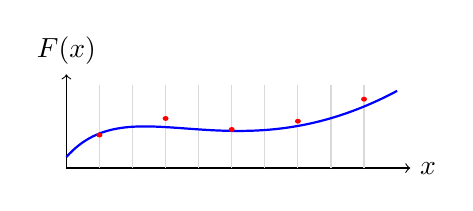
\begin{tikzpicture}[x=0.42cm,y=0.35cm]
 \draw[->] (0,0)--(10.4,0) node[right] {$x$};
 \draw[->] (0,0)--(0,3.4) node[above] {$F(x)$};
 \foreach \x in {1,...,9} {\draw[gray!30] (\x,0)--(\x,3);}
 \draw[blue,thick] (0,0.4) .. controls (2,3.1) and (5,-0.4) .. (10,2.8);
 \foreach \x/\y in {1/1.2,3/1.8,5/1.4,7/1.7,9/2.5}
   \fill[red] (\x,\y) circle (0.09);
\end{tikzpicture}
\end{center}
The next comparison uses Theorem~\ref{thm:116} and Equation~\ref{eq:117}. The proof separates the algebraic estimate from the geometric example. This makes the document useful for edits to prose, formulas, headings and diagrams, while retaining enough ordinary text to exercise paragraph breaking and natural pagination.

\lipsum[13]

\section{A changing estimate: case 119}\label{unit:118}
An observer can return to an earlier part of the document while compilation continues. The relevant statement, equation and hyperlink must still belong to the page actually displayed, including when line wrapping pushes a later theorem across a page boundary.

\lipsum[25-26]
\begin{align}\label{eq:118}
 F_k(x+h)&=F_k(x)+hF_k'(x)+\frac{h^2}{2}F_k''(x)+O(h^3),\\
 \int_0^1 t^k(1-t)\,dt&=\frac{1}{(k+1)(k+2)}.
\end{align}
\begin{theorem}\label{thm:118}
For the finite family in case 119, the normalized error is bounded by $C_k h^2$ whenever $0<h<1$. The constant may depend on $k$ but is independent of the location of the edited paragraph.
\end{theorem}
\begin{proof}
Expand the two terms, collect their first-order contributions, and apply the
triangle inequality. The remaining integral is bounded on the compact interval,
so the asserted estimate follows. This argument also applies after a line break
moves the statement to the next page.
\end{proof}
The next comparison uses Theorem~\ref{thm:117} and Equation~\ref{eq:118}. A local change should remain attached to its source even when surrounding material moves. We compare the displayed argument with the current source version, rather than treating the last compiled page number as a permanent identity.

\lipsum[18]

\section{A changing estimate: case 120}\label{unit:119}
The proof separates the algebraic estimate from the geometric example. This makes the document useful for edits to prose, formulas, headings and diagrams, while retaining enough ordinary text to exercise paragraph breaking and natural pagination.

\lipsum[28-29]
\begin{align}\label{eq:119}
 F_k(x+h)&=F_k(x)+hF_k'(x)+\frac{h^2}{2}F_k''(x)+O(h^3),\\
 \int_0^1 t^k(1-t)\,dt&=\frac{1}{(k+1)(k+2)}.
\end{align}
\begin{theorem}\label{thm:119}
For the finite family in case 120, the normalized error is bounded by $C_k h^2$ whenever $0<h<1$. The constant may depend on $k$ but is independent of the location of the edited paragraph.
\end{theorem}
\begin{proof}
Expand the two terms, collect their first-order contributions, and apply the
triangle inequality. The remaining integral is bounded on the compact interval,
so the asserted estimate follows. This argument also applies after a line break
moves the statement to the next page.
\end{proof}
The next comparison uses Theorem~\ref{thm:118} and Equation~\ref{eq:119}. The construction uses a finite family of examples with different paragraph lengths. Some sentences are short. Others follow the dependence of an estimate on its parameters, introduce a counterexample, and explain why a nearby bound must be reconsidered after an insertion.

\lipsum[23]

\section{A changing estimate: case 121}\label{unit:120}
A local change should remain attached to its source even when surrounding material moves. We compare the displayed argument with the current source version, rather than treating the last compiled page number as a permanent identity.

\lipsum[1-2]
\begin{align}\label{eq:120}
 F_k(x+h)&=F_k(x)+hF_k'(x)+\frac{h^2}{2}F_k''(x)+O(h^3),\\
 \int_0^1 t^k(1-t)\,dt&=\frac{1}{(k+1)(k+2)}.
\end{align}
\begin{lemma}\label{thm:120}
For the finite family in case 121, the normalized error is bounded by $C_k h^2$ whenever $0<h<1$. The constant may depend on $k$ but is independent of the location of the edited paragraph.
\end{lemma}
\begin{proof}
Expand the two terms, collect their first-order contributions, and apply the
triangle inequality. The remaining integral is bounded on the compact interval,
so the asserted estimate follows. This argument also applies after a line break
moves the statement to the next page.
\end{proof}
The next comparison uses Theorem~\ref{thm:119} and Equation~\ref{eq:120}. An observer can return to an earlier part of the document while compilation continues. The relevant statement, equation and hyperlink must still belong to the page actually displayed, including when line wrapping pushes a later theorem across a page boundary.

\lipsum[3]

\section{A changing estimate: case 122}\label{unit:121}
The construction uses a finite family of examples with different paragraph lengths. Some sentences are short. Others follow the dependence of an estimate on its parameters, introduce a counterexample, and explain why a nearby bound must be reconsidered after an insertion.

\lipsum[4-5]
\begin{align}\label{eq:121}
 F_k(x+h)&=F_k(x)+hF_k'(x)+\frac{h^2}{2}F_k''(x)+O(h^3),\\
 \int_0^1 t^k(1-t)\,dt&=\frac{1}{(k+1)(k+2)}.
\end{align}
\begin{theorem}\label{thm:121}
For the finite family in case 122, the normalized error is bounded by $C_k h^2$ whenever $0<h<1$. The constant may depend on $k$ but is independent of the location of the edited paragraph.
\end{theorem}
\begin{proof}
Expand the two terms, collect their first-order contributions, and apply the
triangle inequality. The remaining integral is bounded on the compact interval,
so the asserted estimate follows. This argument also applies after a line break
moves the statement to the next page.
\end{proof}
The next comparison uses Theorem~\ref{thm:120} and Equation~\ref{eq:121}. The proof separates the algebraic estimate from the geometric example. This makes the document useful for edits to prose, formulas, headings and diagrams, while retaining enough ordinary text to exercise paragraph breaking and natural pagination.

\lipsum[8]

\section{A changing estimate: case 123}\label{unit:122}
An observer can return to an earlier part of the document while compilation continues. The relevant statement, equation and hyperlink must still belong to the page actually displayed, including when line wrapping pushes a later theorem across a page boundary.

\lipsum[7-8]
\begin{align}\label{eq:122}
 F_k(x+h)&=F_k(x)+hF_k'(x)+\frac{h^2}{2}F_k''(x)+O(h^3),\\
 \int_0^1 t^k(1-t)\,dt&=\frac{1}{(k+1)(k+2)}.
\end{align}
\begin{theorem}\label{thm:122}
For the finite family in case 123, the normalized error is bounded by $C_k h^2$ whenever $0<h<1$. The constant may depend on $k$ but is independent of the location of the edited paragraph.
\end{theorem}
\begin{proof}
Expand the two terms, collect their first-order contributions, and apply the
triangle inequality. The remaining integral is bounded on the compact interval,
so the asserted estimate follows. This argument also applies after a line break
moves the statement to the next page.
\end{proof}
The next comparison uses Theorem~\ref{thm:121} and Equation~\ref{eq:122}. A local change should remain attached to its source even when surrounding material moves. We compare the displayed argument with the current source version, rather than treating the last compiled page number as a permanent identity.

\lipsum[13]

\section{A changing estimate: case 124}\label{unit:123}
The proof separates the algebraic estimate from the geometric example. This makes the document useful for edits to prose, formulas, headings and diagrams, while retaining enough ordinary text to exercise paragraph breaking and natural pagination.

\lipsum[10-11]
\begin{align}\label{eq:123}
 F_k(x+h)&=F_k(x)+hF_k'(x)+\frac{h^2}{2}F_k''(x)+O(h^3),\\
 \int_0^1 t^k(1-t)\,dt&=\frac{1}{(k+1)(k+2)}.
\end{align}
\begin{lemma}\label{thm:123}
For the finite family in case 124, the normalized error is bounded by $C_k h^2$ whenever $0<h<1$. The constant may depend on $k$ but is independent of the location of the edited paragraph.
\end{lemma}
\begin{proof}
Expand the two terms, collect their first-order contributions, and apply the
triangle inequality. The remaining integral is bounded on the compact interval,
so the asserted estimate follows. This argument also applies after a line break
moves the statement to the next page.
\end{proof}
\begin{center}
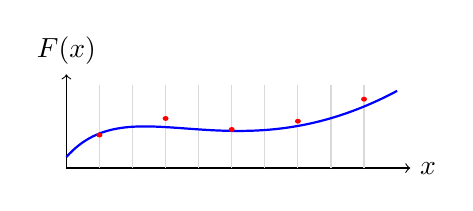
\begin{tikzpicture}[x=0.42cm,y=0.35cm]
 \draw[->] (0,0)--(10.4,0) node[right] {$x$};
 \draw[->] (0,0)--(0,3.4) node[above] {$F(x)$};
 \foreach \x in {1,...,9} {\draw[gray!30] (\x,0)--(\x,3);}
 \draw[blue,thick] (0,0.4) .. controls (2,3.1) and (5,-0.4) .. (10,2.8);
 \foreach \x/\y in {1/1.2,3/1.8,5/1.4,7/1.7,9/2.5}
   \fill[red] (\x,\y) circle (0.09);
\end{tikzpicture}
\end{center}
The next comparison uses Theorem~\ref{thm:122} and Equation~\ref{eq:123}. The construction uses a finite family of examples with different paragraph lengths. Some sentences are short. Others follow the dependence of an estimate on its parameters, introduce a counterexample, and explain why a nearby bound must be reconsidered after an insertion.

\lipsum[18]

\section{A changing estimate: case 125}\label{unit:124}
A local change should remain attached to its source even when surrounding material moves. We compare the displayed argument with the current source version, rather than treating the last compiled page number as a permanent identity.

\lipsum[13-14]
\begin{align}\label{eq:124}
 F_k(x+h)&=F_k(x)+hF_k'(x)+\frac{h^2}{2}F_k''(x)+O(h^3),\\
 \int_0^1 t^k(1-t)\,dt&=\frac{1}{(k+1)(k+2)}.
\end{align}
\begin{theorem}\label{thm:124}
For the finite family in case 125, the normalized error is bounded by $C_k h^2$ whenever $0<h<1$. The constant may depend on $k$ but is independent of the location of the edited paragraph.
\end{theorem}
\begin{proof}
Expand the two terms, collect their first-order contributions, and apply the
triangle inequality. The remaining integral is bounded on the compact interval,
so the asserted estimate follows. This argument also applies after a line break
moves the statement to the next page.
\end{proof}
The next comparison uses Theorem~\ref{thm:123} and Equation~\ref{eq:124}. An observer can return to an earlier part of the document while compilation continues. The relevant statement, equation and hyperlink must still belong to the page actually displayed, including when line wrapping pushes a later theorem across a page boundary.

\lipsum[23]

\section{A changing estimate: case 126}\label{unit:125}
The construction uses a finite family of examples with different paragraph lengths. Some sentences are short. Others follow the dependence of an estimate on its parameters, introduce a counterexample, and explain why a nearby bound must be reconsidered after an insertion.

\lipsum[16-17]
\begin{align}\label{eq:125}
 F_k(x+h)&=F_k(x)+hF_k'(x)+\frac{h^2}{2}F_k''(x)+O(h^3),\\
 \int_0^1 t^k(1-t)\,dt&=\frac{1}{(k+1)(k+2)}.
\end{align}
\begin{theorem}\label{thm:125}
For the finite family in case 126, the normalized error is bounded by $C_k h^2$ whenever $0<h<1$. The constant may depend on $k$ but is independent of the location of the edited paragraph.
\end{theorem}
\begin{proof}
Expand the two terms, collect their first-order contributions, and apply the
triangle inequality. The remaining integral is bounded on the compact interval,
so the asserted estimate follows. This argument also applies after a line break
moves the statement to the next page.
\end{proof}
The next comparison uses Theorem~\ref{thm:124} and Equation~\ref{eq:125}. The proof separates the algebraic estimate from the geometric example. This makes the document useful for edits to prose, formulas, headings and diagrams, while retaining enough ordinary text to exercise paragraph breaking and natural pagination.

\lipsum[3]

\section{A changing estimate: case 127}\label{unit:126}
An observer can return to an earlier part of the document while compilation continues. The relevant statement, equation and hyperlink must still belong to the page actually displayed, including when line wrapping pushes a later theorem across a page boundary.

\lipsum[19-20]
\begin{align}\label{eq:126}
 F_k(x+h)&=F_k(x)+hF_k'(x)+\frac{h^2}{2}F_k''(x)+O(h^3),\\
 \int_0^1 t^k(1-t)\,dt&=\frac{1}{(k+1)(k+2)}.
\end{align}
\begin{lemma}\label{thm:126}
For the finite family in case 127, the normalized error is bounded by $C_k h^2$ whenever $0<h<1$. The constant may depend on $k$ but is independent of the location of the edited paragraph.
\end{lemma}
\begin{proof}
Expand the two terms, collect their first-order contributions, and apply the
triangle inequality. The remaining integral is bounded on the compact interval,
so the asserted estimate follows. This argument also applies after a line break
moves the statement to the next page.
\end{proof}
The next comparison uses Theorem~\ref{thm:125} and Equation~\ref{eq:126}. A local change should remain attached to its source even when surrounding material moves. We compare the displayed argument with the current source version, rather than treating the last compiled page number as a permanent identity.

\lipsum[8]

\section{A changing estimate: case 128}\label{unit:127}
The proof separates the algebraic estimate from the geometric example. This makes the document useful for edits to prose, formulas, headings and diagrams, while retaining enough ordinary text to exercise paragraph breaking and natural pagination.

\lipsum[22-23]
\begin{align}\label{eq:127}
 F_k(x+h)&=F_k(x)+hF_k'(x)+\frac{h^2}{2}F_k''(x)+O(h^3),\\
 \int_0^1 t^k(1-t)\,dt&=\frac{1}{(k+1)(k+2)}.
\end{align}
\begin{theorem}\label{thm:127}
For the finite family in case 128, the normalized error is bounded by $C_k h^2$ whenever $0<h<1$. The constant may depend on $k$ but is independent of the location of the edited paragraph.
\end{theorem}
\begin{proof}
Expand the two terms, collect their first-order contributions, and apply the
triangle inequality. The remaining integral is bounded on the compact interval,
so the asserted estimate follows. This argument also applies after a line break
moves the statement to the next page.
\end{proof}
The next comparison uses Theorem~\ref{thm:126} and Equation~\ref{eq:127}. The construction uses a finite family of examples with different paragraph lengths. Some sentences are short. Others follow the dependence of an estimate on its parameters, introduce a counterexample, and explain why a nearby bound must be reconsidered after an insertion.

\lipsum[13]

\section{A changing estimate: case 129}\label{unit:128}
A local change should remain attached to its source even when surrounding material moves. We compare the displayed argument with the current source version, rather than treating the last compiled page number as a permanent identity.

\lipsum[25-26]
\begin{align}\label{eq:128}
 F_k(x+h)&=F_k(x)+hF_k'(x)+\frac{h^2}{2}F_k''(x)+O(h^3),\\
 \int_0^1 t^k(1-t)\,dt&=\frac{1}{(k+1)(k+2)}.
\end{align}
\begin{theorem}\label{thm:128}
For the finite family in case 129, the normalized error is bounded by $C_k h^2$ whenever $0<h<1$. The constant may depend on $k$ but is independent of the location of the edited paragraph.
\end{theorem}
\begin{proof}
Expand the two terms, collect their first-order contributions, and apply the
triangle inequality. The remaining integral is bounded on the compact interval,
so the asserted estimate follows. This argument also applies after a line break
moves the statement to the next page.
\end{proof}
The next comparison uses Theorem~\ref{thm:127} and Equation~\ref{eq:128}. An observer can return to an earlier part of the document while compilation continues. The relevant statement, equation and hyperlink must still belong to the page actually displayed, including when line wrapping pushes a later theorem across a page boundary.

\lipsum[18]

\section{A changing estimate: case 130}\label{unit:129}
The construction uses a finite family of examples with different paragraph lengths. Some sentences are short. Others follow the dependence of an estimate on its parameters, introduce a counterexample, and explain why a nearby bound must be reconsidered after an insertion.

\lipsum[28-29]
\begin{align}\label{eq:129}
 F_k(x+h)&=F_k(x)+hF_k'(x)+\frac{h^2}{2}F_k''(x)+O(h^3),\\
 \int_0^1 t^k(1-t)\,dt&=\frac{1}{(k+1)(k+2)}.
\end{align}
\begin{lemma}\label{thm:129}
For the finite family in case 130, the normalized error is bounded by $C_k h^2$ whenever $0<h<1$. The constant may depend on $k$ but is independent of the location of the edited paragraph.
\end{lemma}
\begin{proof}
Expand the two terms, collect their first-order contributions, and apply the
triangle inequality. The remaining integral is bounded on the compact interval,
so the asserted estimate follows. This argument also applies after a line break
moves the statement to the next page.
\end{proof}
\begin{center}
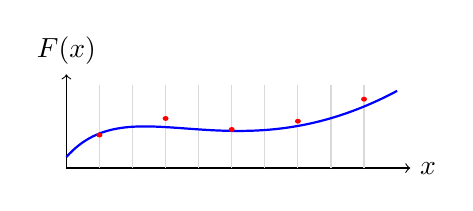
\begin{tikzpicture}[x=0.42cm,y=0.35cm]
 \draw[->] (0,0)--(10.4,0) node[right] {$x$};
 \draw[->] (0,0)--(0,3.4) node[above] {$F(x)$};
 \foreach \x in {1,...,9} {\draw[gray!30] (\x,0)--(\x,3);}
 \draw[blue,thick] (0,0.4) .. controls (2,3.1) and (5,-0.4) .. (10,2.8);
 \foreach \x/\y in {1/1.2,3/1.8,5/1.4,7/1.7,9/2.5}
   \fill[red] (\x,\y) circle (0.09);
\end{tikzpicture}
\end{center}
The next comparison uses Theorem~\ref{thm:128} and Equation~\ref{eq:129}. The proof separates the algebraic estimate from the geometric example. This makes the document useful for edits to prose, formulas, headings and diagrams, while retaining enough ordinary text to exercise paragraph breaking and natural pagination.

\lipsum[23]

\section{A changing estimate: case 131}\label{unit:130}
An observer can return to an earlier part of the document while compilation continues. The relevant statement, equation and hyperlink must still belong to the page actually displayed, including when line wrapping pushes a later theorem across a page boundary.

\lipsum[1-2]
\begin{align}\label{eq:130}
 F_k(x+h)&=F_k(x)+hF_k'(x)+\frac{h^2}{2}F_k''(x)+O(h^3),\\
 \int_0^1 t^k(1-t)\,dt&=\frac{1}{(k+1)(k+2)}.
\end{align}
\begin{theorem}\label{thm:130}
For the finite family in case 131, the normalized error is bounded by $C_k h^2$ whenever $0<h<1$. The constant may depend on $k$ but is independent of the location of the edited paragraph.
\end{theorem}
\begin{proof}
Expand the two terms, collect their first-order contributions, and apply the
triangle inequality. The remaining integral is bounded on the compact interval,
so the asserted estimate follows. This argument also applies after a line break
moves the statement to the next page.
\end{proof}
The next comparison uses Theorem~\ref{thm:129} and Equation~\ref{eq:130}. A local change should remain attached to its source even when surrounding material moves. We compare the displayed argument with the current source version, rather than treating the last compiled page number as a permanent identity.

\lipsum[3]

\section{A changing estimate: case 132}\label{unit:131}
The proof separates the algebraic estimate from the geometric example. This makes the document useful for edits to prose, formulas, headings and diagrams, while retaining enough ordinary text to exercise paragraph breaking and natural pagination.

\lipsum[4-5]
\begin{align}\label{eq:131}
 F_k(x+h)&=F_k(x)+hF_k'(x)+\frac{h^2}{2}F_k''(x)+O(h^3),\\
 \int_0^1 t^k(1-t)\,dt&=\frac{1}{(k+1)(k+2)}.
\end{align}
\begin{theorem}\label{thm:131}
For the finite family in case 132, the normalized error is bounded by $C_k h^2$ whenever $0<h<1$. The constant may depend on $k$ but is independent of the location of the edited paragraph.
\end{theorem}
\begin{proof}
Expand the two terms, collect their first-order contributions, and apply the
triangle inequality. The remaining integral is bounded on the compact interval,
so the asserted estimate follows. This argument also applies after a line break
moves the statement to the next page.
\end{proof}
The next comparison uses Theorem~\ref{thm:130} and Equation~\ref{eq:131}. The construction uses a finite family of examples with different paragraph lengths. Some sentences are short. Others follow the dependence of an estimate on its parameters, introduce a counterexample, and explain why a nearby bound must be reconsidered after an insertion.

\lipsum[8]

\section{A changing estimate: case 133}\label{unit:132}
A local change should remain attached to its source even when surrounding material moves. We compare the displayed argument with the current source version, rather than treating the last compiled page number as a permanent identity.

\lipsum[7-8]
\begin{align}\label{eq:132}
 F_k(x+h)&=F_k(x)+hF_k'(x)+\frac{h^2}{2}F_k''(x)+O(h^3),\\
 \int_0^1 t^k(1-t)\,dt&=\frac{1}{(k+1)(k+2)}.
\end{align}
\begin{lemma}\label{thm:132}
For the finite family in case 133, the normalized error is bounded by $C_k h^2$ whenever $0<h<1$. The constant may depend on $k$ but is independent of the location of the edited paragraph.
\end{lemma}
\begin{proof}
Expand the two terms, collect their first-order contributions, and apply the
triangle inequality. The remaining integral is bounded on the compact interval,
so the asserted estimate follows. This argument also applies after a line break
moves the statement to the next page.
\end{proof}
The next comparison uses Theorem~\ref{thm:131} and Equation~\ref{eq:132}. An observer can return to an earlier part of the document while compilation continues. The relevant statement, equation and hyperlink must still belong to the page actually displayed, including when line wrapping pushes a later theorem across a page boundary.

\lipsum[13]

\section{A changing estimate: case 134}\label{unit:133}
The construction uses a finite family of examples with different paragraph lengths. Some sentences are short. Others follow the dependence of an estimate on its parameters, introduce a counterexample, and explain why a nearby bound must be reconsidered after an insertion.

\lipsum[10-11]
\begin{align}\label{eq:133}
 F_k(x+h)&=F_k(x)+hF_k'(x)+\frac{h^2}{2}F_k''(x)+O(h^3),\\
 \int_0^1 t^k(1-t)\,dt&=\frac{1}{(k+1)(k+2)}.
\end{align}
\begin{theorem}\label{thm:133}
For the finite family in case 134, the normalized error is bounded by $C_k h^2$ whenever $0<h<1$. The constant may depend on $k$ but is independent of the location of the edited paragraph.
\end{theorem}
\begin{proof}
Expand the two terms, collect their first-order contributions, and apply the
triangle inequality. The remaining integral is bounded on the compact interval,
so the asserted estimate follows. This argument also applies after a line break
moves the statement to the next page.
\end{proof}
The next comparison uses Theorem~\ref{thm:132} and Equation~\ref{eq:133}. The proof separates the algebraic estimate from the geometric example. This makes the document useful for edits to prose, formulas, headings and diagrams, while retaining enough ordinary text to exercise paragraph breaking and natural pagination.

\lipsum[18]

\section{A changing estimate: case 135}\label{unit:134}
An observer can return to an earlier part of the document while compilation continues. The relevant statement, equation and hyperlink must still belong to the page actually displayed, including when line wrapping pushes a later theorem across a page boundary.

\lipsum[13-14]
\begin{align}\label{eq:134}
 F_k(x+h)&=F_k(x)+hF_k'(x)+\frac{h^2}{2}F_k''(x)+O(h^3),\\
 \int_0^1 t^k(1-t)\,dt&=\frac{1}{(k+1)(k+2)}.
\end{align}
\begin{theorem}\label{thm:134}
For the finite family in case 135, the normalized error is bounded by $C_k h^2$ whenever $0<h<1$. The constant may depend on $k$ but is independent of the location of the edited paragraph.
\end{theorem}
\begin{proof}
Expand the two terms, collect their first-order contributions, and apply the
triangle inequality. The remaining integral is bounded on the compact interval,
so the asserted estimate follows. This argument also applies after a line break
moves the statement to the next page.
\end{proof}
The next comparison uses Theorem~\ref{thm:133} and Equation~\ref{eq:134}. A local change should remain attached to its source even when surrounding material moves. We compare the displayed argument with the current source version, rather than treating the last compiled page number as a permanent identity.

\lipsum[23]

\section{A changing estimate: case 136}\label{unit:135}
The proof separates the algebraic estimate from the geometric example. This makes the document useful for edits to prose, formulas, headings and diagrams, while retaining enough ordinary text to exercise paragraph breaking and natural pagination.

\lipsum[16-17]
\begin{align}\label{eq:135}
 F_k(x+h)&=F_k(x)+hF_k'(x)+\frac{h^2}{2}F_k''(x)+O(h^3),\\
 \int_0^1 t^k(1-t)\,dt&=\frac{1}{(k+1)(k+2)}.
\end{align}
\begin{lemma}\label{thm:135}
For the finite family in case 136, the normalized error is bounded by $C_k h^2$ whenever $0<h<1$. The constant may depend on $k$ but is independent of the location of the edited paragraph.
\end{lemma}
\begin{proof}
Expand the two terms, collect their first-order contributions, and apply the
triangle inequality. The remaining integral is bounded on the compact interval,
so the asserted estimate follows. This argument also applies after a line break
moves the statement to the next page.
\end{proof}
\begin{center}
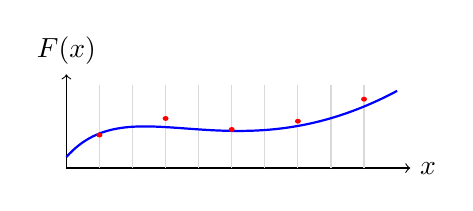
\begin{tikzpicture}[x=0.42cm,y=0.35cm]
 \draw[->] (0,0)--(10.4,0) node[right] {$x$};
 \draw[->] (0,0)--(0,3.4) node[above] {$F(x)$};
 \foreach \x in {1,...,9} {\draw[gray!30] (\x,0)--(\x,3);}
 \draw[blue,thick] (0,0.4) .. controls (2,3.1) and (5,-0.4) .. (10,2.8);
 \foreach \x/\y in {1/1.2,3/1.8,5/1.4,7/1.7,9/2.5}
   \fill[red] (\x,\y) circle (0.09);
\end{tikzpicture}
\end{center}
The next comparison uses Theorem~\ref{thm:134} and Equation~\ref{eq:135}. The construction uses a finite family of examples with different paragraph lengths. Some sentences are short. Others follow the dependence of an estimate on its parameters, introduce a counterexample, and explain why a nearby bound must be reconsidered after an insertion.

\lipsum[3]

\section{A changing estimate: case 137}\label{unit:136}
A local change should remain attached to its source even when surrounding material moves. We compare the displayed argument with the current source version, rather than treating the last compiled page number as a permanent identity.

\lipsum[19-20]
\begin{align}\label{eq:136}
 F_k(x+h)&=F_k(x)+hF_k'(x)+\frac{h^2}{2}F_k''(x)+O(h^3),\\
 \int_0^1 t^k(1-t)\,dt&=\frac{1}{(k+1)(k+2)}.
\end{align}
\begin{theorem}\label{thm:136}
For the finite family in case 137, the normalized error is bounded by $C_k h^2$ whenever $0<h<1$. The constant may depend on $k$ but is independent of the location of the edited paragraph.
\end{theorem}
\begin{proof}
Expand the two terms, collect their first-order contributions, and apply the
triangle inequality. The remaining integral is bounded on the compact interval,
so the asserted estimate follows. This argument also applies after a line break
moves the statement to the next page.
\end{proof}
The next comparison uses Theorem~\ref{thm:135} and Equation~\ref{eq:136}. An observer can return to an earlier part of the document while compilation continues. The relevant statement, equation and hyperlink must still belong to the page actually displayed, including when line wrapping pushes a later theorem across a page boundary.

\lipsum[8]

\section{A changing estimate: case 138}\label{unit:137}
The construction uses a finite family of examples with different paragraph lengths. Some sentences are short. Others follow the dependence of an estimate on its parameters, introduce a counterexample, and explain why a nearby bound must be reconsidered after an insertion.

\lipsum[22-23]
\begin{align}\label{eq:137}
 F_k(x+h)&=F_k(x)+hF_k'(x)+\frac{h^2}{2}F_k''(x)+O(h^3),\\
 \int_0^1 t^k(1-t)\,dt&=\frac{1}{(k+1)(k+2)}.
\end{align}
\begin{theorem}\label{thm:137}
For the finite family in case 138, the normalized error is bounded by $C_k h^2$ whenever $0<h<1$. The constant may depend on $k$ but is independent of the location of the edited paragraph.
\end{theorem}
\begin{proof}
Expand the two terms, collect their first-order contributions, and apply the
triangle inequality. The remaining integral is bounded on the compact interval,
so the asserted estimate follows. This argument also applies after a line break
moves the statement to the next page.
\end{proof}
The next comparison uses Theorem~\ref{thm:136} and Equation~\ref{eq:137}. The proof separates the algebraic estimate from the geometric example. This makes the document useful for edits to prose, formulas, headings and diagrams, while retaining enough ordinary text to exercise paragraph breaking and natural pagination.

\lipsum[13]

\section{A changing estimate: case 139}\label{unit:138}
An observer can return to an earlier part of the document while compilation continues. The relevant statement, equation and hyperlink must still belong to the page actually displayed, including when line wrapping pushes a later theorem across a page boundary.

\lipsum[25-26]
\begin{align}\label{eq:138}
 F_k(x+h)&=F_k(x)+hF_k'(x)+\frac{h^2}{2}F_k''(x)+O(h^3),\\
 \int_0^1 t^k(1-t)\,dt&=\frac{1}{(k+1)(k+2)}.
\end{align}
\begin{lemma}\label{thm:138}
For the finite family in case 139, the normalized error is bounded by $C_k h^2$ whenever $0<h<1$. The constant may depend on $k$ but is independent of the location of the edited paragraph.
\end{lemma}
\begin{proof}
Expand the two terms, collect their first-order contributions, and apply the
triangle inequality. The remaining integral is bounded on the compact interval,
so the asserted estimate follows. This argument also applies after a line break
moves the statement to the next page.
\end{proof}
The next comparison uses Theorem~\ref{thm:137} and Equation~\ref{eq:138}. A local change should remain attached to its source even when surrounding material moves. We compare the displayed argument with the current source version, rather than treating the last compiled page number as a permanent identity.

\lipsum[18]

\section{A changing estimate: case 140}\label{unit:139}
The proof separates the algebraic estimate from the geometric example. This makes the document useful for edits to prose, formulas, headings and diagrams, while retaining enough ordinary text to exercise paragraph breaking and natural pagination.

\lipsum[28-29]
\begin{align}\label{eq:139}
 F_k(x+h)&=F_k(x)+hF_k'(x)+\frac{h^2}{2}F_k''(x)+O(h^3),\\
 \int_0^1 t^k(1-t)\,dt&=\frac{1}{(k+1)(k+2)}.
\end{align}
\begin{theorem}\label{thm:139}
For the finite family in case 140, the normalized error is bounded by $C_k h^2$ whenever $0<h<1$. The constant may depend on $k$ but is independent of the location of the edited paragraph.
\end{theorem}
\begin{proof}
Expand the two terms, collect their first-order contributions, and apply the
triangle inequality. The remaining integral is bounded on the compact interval,
so the asserted estimate follows. This argument also applies after a line break
moves the statement to the next page.
\end{proof}
The next comparison uses Theorem~\ref{thm:138} and Equation~\ref{eq:139}. The construction uses a finite family of examples with different paragraph lengths. Some sentences are short. Others follow the dependence of an estimate on its parameters, introduce a counterexample, and explain why a nearby bound must be reconsidered after an insertion.

\lipsum[23]

\section{A changing estimate: case 141}\label{unit:140}
A local change should remain attached to its source even when surrounding material moves. We compare the displayed argument with the current source version, rather than treating the last compiled page number as a permanent identity.

\lipsum[1-2]
\begin{align}\label{eq:140}
 F_k(x+h)&=F_k(x)+hF_k'(x)+\frac{h^2}{2}F_k''(x)+O(h^3),\\
 \int_0^1 t^k(1-t)\,dt&=\frac{1}{(k+1)(k+2)}.
\end{align}
\begin{theorem}\label{thm:140}
For the finite family in case 141, the normalized error is bounded by $C_k h^2$ whenever $0<h<1$. The constant may depend on $k$ but is independent of the location of the edited paragraph.
\end{theorem}
\begin{proof}
Expand the two terms, collect their first-order contributions, and apply the
triangle inequality. The remaining integral is bounded on the compact interval,
so the asserted estimate follows. This argument also applies after a line break
moves the statement to the next page.
\end{proof}
The next comparison uses Theorem~\ref{thm:139} and Equation~\ref{eq:140}. An observer can return to an earlier part of the document while compilation continues. The relevant statement, equation and hyperlink must still belong to the page actually displayed, including when line wrapping pushes a later theorem across a page boundary.

\lipsum[3]

\section{A changing estimate: case 142}\label{unit:141}
The construction uses a finite family of examples with different paragraph lengths. Some sentences are short. Others follow the dependence of an estimate on its parameters, introduce a counterexample, and explain why a nearby bound must be reconsidered after an insertion.

\lipsum[4-5]
\begin{align}\label{eq:141}
 F_k(x+h)&=F_k(x)+hF_k'(x)+\frac{h^2}{2}F_k''(x)+O(h^3),\\
 \int_0^1 t^k(1-t)\,dt&=\frac{1}{(k+1)(k+2)}.
\end{align}
\begin{lemma}\label{thm:141}
For the finite family in case 142, the normalized error is bounded by $C_k h^2$ whenever $0<h<1$. The constant may depend on $k$ but is independent of the location of the edited paragraph.
\end{lemma}
\begin{proof}
Expand the two terms, collect their first-order contributions, and apply the
triangle inequality. The remaining integral is bounded on the compact interval,
so the asserted estimate follows. This argument also applies after a line break
moves the statement to the next page.
\end{proof}
\begin{center}
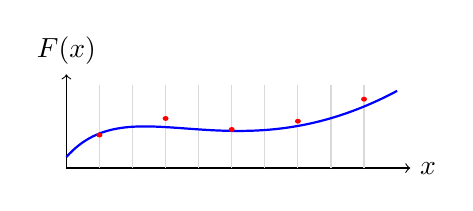
\begin{tikzpicture}[x=0.42cm,y=0.35cm]
 \draw[->] (0,0)--(10.4,0) node[right] {$x$};
 \draw[->] (0,0)--(0,3.4) node[above] {$F(x)$};
 \foreach \x in {1,...,9} {\draw[gray!30] (\x,0)--(\x,3);}
 \draw[blue,thick] (0,0.4) .. controls (2,3.1) and (5,-0.4) .. (10,2.8);
 \foreach \x/\y in {1/1.2,3/1.8,5/1.4,7/1.7,9/2.5}
   \fill[red] (\x,\y) circle (0.09);
\end{tikzpicture}
\end{center}
The next comparison uses Theorem~\ref{thm:140} and Equation~\ref{eq:141}. The proof separates the algebraic estimate from the geometric example. This makes the document useful for edits to prose, formulas, headings and diagrams, while retaining enough ordinary text to exercise paragraph breaking and natural pagination.

\lipsum[8]

\section{A changing estimate: case 143}\label{unit:142}
An observer can return to an earlier part of the document while compilation continues. The relevant statement, equation and hyperlink must still belong to the page actually displayed, including when line wrapping pushes a later theorem across a page boundary.

\lipsum[7-8]
\begin{align}\label{eq:142}
 F_k(x+h)&=F_k(x)+hF_k'(x)+\frac{h^2}{2}F_k''(x)+O(h^3),\\
 \int_0^1 t^k(1-t)\,dt&=\frac{1}{(k+1)(k+2)}.
\end{align}
\begin{theorem}\label{thm:142}
For the finite family in case 143, the normalized error is bounded by $C_k h^2$ whenever $0<h<1$. The constant may depend on $k$ but is independent of the location of the edited paragraph.
\end{theorem}
\begin{proof}
Expand the two terms, collect their first-order contributions, and apply the
triangle inequality. The remaining integral is bounded on the compact interval,
so the asserted estimate follows. This argument also applies after a line break
moves the statement to the next page.
\end{proof}
The next comparison uses Theorem~\ref{thm:141} and Equation~\ref{eq:142}. A local change should remain attached to its source even when surrounding material moves. We compare the displayed argument with the current source version, rather than treating the last compiled page number as a permanent identity.

\lipsum[13]

\section{A changing estimate: case 144}\label{unit:143}
\hypertarget{varied:late}{}\label{anchor:late}
\noindent \texttt{LATE-0143}: This uniquely marked paragraph remains visible as nearby text, mathematical statements and section boundaries change.
%<VARIED-CURSOR:late>

The proof separates the algebraic estimate from the geometric example. This makes the document useful for edits to prose, formulas, headings and diagrams, while retaining enough ordinary text to exercise paragraph breaking and natural pagination.

\lipsum[10-11]
\begin{align}\label{eq:143}
 F_k(x+h)&=F_k(x)+hF_k'(x)+\frac{h^2}{2}F_k''(x)+O(h^3),\\
 \int_0^1 t^k(1-t)\,dt&=\frac{1}{(k+1)(k+2)}.
\end{align}
\begin{theorem}\label{thm:143}
For the finite family in case 144, the normalized error is bounded by $C_k h^2$ whenever $0<h<1$. The constant may depend on $k$ but is independent of the location of the edited paragraph.
\end{theorem}
\begin{proof}
Expand the two terms, collect their first-order contributions, and apply the
triangle inequality. The remaining integral is bounded on the compact interval,
so the asserted estimate follows. This argument also applies after a line break
moves the statement to the next page.
\end{proof}
The next comparison uses Theorem~\ref{thm:142} and Equation~\ref{eq:143}. The construction uses a finite family of examples with different paragraph lengths. Some sentences are short. Others follow the dependence of an estimate on its parameters, introduce a counterexample, and explain why a nearby bound must be reconsidered after an insertion.

\lipsum[18]

\section{A changing estimate: case 145}\label{unit:144}
A local change should remain attached to its source even when surrounding material moves. We compare the displayed argument with the current source version, rather than treating the last compiled page number as a permanent identity.

\lipsum[13-14]
\begin{align}\label{eq:144}
 F_k(x+h)&=F_k(x)+hF_k'(x)+\frac{h^2}{2}F_k''(x)+O(h^3),\\
 \int_0^1 t^k(1-t)\,dt&=\frac{1}{(k+1)(k+2)}.
\end{align}
\begin{lemma}\label{thm:144}
For the finite family in case 145, the normalized error is bounded by $C_k h^2$ whenever $0<h<1$. The constant may depend on $k$ but is independent of the location of the edited paragraph.
\end{lemma}
\begin{proof}
Expand the two terms, collect their first-order contributions, and apply the
triangle inequality. The remaining integral is bounded on the compact interval,
so the asserted estimate follows. This argument also applies after a line break
moves the statement to the next page.
\end{proof}
The next comparison uses Theorem~\ref{thm:143} and Equation~\ref{eq:144}. An observer can return to an earlier part of the document while compilation continues. The relevant statement, equation and hyperlink must still belong to the page actually displayed, including when line wrapping pushes a later theorem across a page boundary.

\lipsum[23]

\section*{The end of the experiment}
\hyperref[anchor:early]{Return to the early anchor}; \hyperref[anchor:middle]{return to the middle anchor}; \hyperref[anchor:late]{return to the late anchor}.
\end{document}
